% ONINU study notes -- generated by _work/pipeline/build_tex.py from markdown.
% Compile with:  latexmk -xelatex nelinearno.tex   (lualatex also works)
\documentclass[11pt,a4paper,parskip=half,headsepline,numbers=noenddot]{scrartcl}

% ---------------------------------------------------------------- page layout
\usepackage[a4paper,left=2cm,right=2cm,top=2.4cm,bottom=2.2cm,headheight=15pt,headsep=0.5cm]{geometry}

% ---------------------------------------------------------------- math
\usepackage{amsmath,amssymb}
\usepackage{mathtools}
\usepackage{libertinust1math}  % Libertinus math, matches the text font
\usepackage{bm}

% ---------------------------------------------------------------- fonts and language
\usepackage[no-math]{fontspec}  % no-math: keep the Type1 math fonts set up above
\IfFontExistsTF{LibertinusSerif-Regular.otf}{%
  \setmainfont{LibertinusSerif}[Extension=.otf, UprightFont=*-Regular, BoldFont=*-Bold,
    ItalicFont=*-Italic, BoldItalicFont=*-BoldItalic]
  \setsansfont{LibertinusSans}[Extension=.otf, UprightFont=*-Regular, BoldFont=*-Bold,
    ItalicFont=*-Italic, BoldItalicFont=*-Bold]
}{% fallback: TeX Gyre Pagella / Heros
  \setmainfont{texgyrepagella}[Extension=.otf, UprightFont=*-regular, BoldFont=*-bold,
    ItalicFont=*-italic, BoldItalicFont=*-bolditalic]
  \setsansfont{texgyreheros}[Extension=.otf, UprightFont=*-regular, BoldFont=*-bold,
    ItalicFont=*-italic, BoldItalicFont=*-bolditalic]
}
\setmonofont{lmmono10-regular.otf}[Scale=0.95]
\usepackage[serbian,shorthands=off]{babel}  % Serbian (Latin): Sadržaj, Slika, Tabela
\usepackage{microtype}
\setlength{\emergencystretch}{3em}
% a few Unicode characters that may be typed inside math
\usepackage{newunicodechar}
\newunicodechar{°}{\ifmmode^{\circ}\else\textdegree\fi}
\newunicodechar{≤}{\ensuremath{\leq}}
\newunicodechar{≥}{\ensuremath{\geq}}
\newunicodechar{≠}{\ensuremath{\neq}}
\newunicodechar{≈}{\ensuremath{\approx}}
\newunicodechar{∞}{\ensuremath{\infty}}
\newunicodechar{→}{\ensuremath{\rightarrow}}
\newunicodechar{⇒}{\ensuremath{\Rightarrow}}
\newunicodechar{±}{\ensuremath{\pm}}
\newunicodechar{×}{\ensuremath{\times}}
\newunicodechar{·}{\ensuremath{\cdot}}
\newunicodechar{−}{\ensuremath{-}}
\newunicodechar{ᵀ}{\ensuremath{^{\mathsf{T}}}}

% ---------------------------------------------------------------- colors, boxes
\usepackage{xcolor}
\definecolor{kljucnaC}{HTML}{1F5FA8}
\definecolor{zastoC}{HTML}{2E7D32}
\definecolor{ispitC}{HTML}{C2530A}
\definecolor{izvorC}{HTML}{6B6B6B}
\definecolor{linkC}{HTML}{1A4480}
\usepackage[most]{tcolorbox}
\tcbset{oninu/.style={enhanced, breakable, colback=#1!5, colframe=#1, colbacktitle=#1!14,
    coltitle=#1!75!black, fonttitle=\sffamily\bfseries, boxrule=0.5pt, leftrule=2.5pt,
    arc=1.5pt, left=6pt, right=6pt, top=3pt, bottom=4pt, toptitle=2pt, bottomtitle=2pt,
    before skip=8pt, after skip=10pt, parbox=false}}
% \begin{kljucna}[optional subtitle] ... \end{kljucna}   (same for zasto, ispit)
\newcommand*{\oninutitle}[2]{#1\ifx\relax#2\relax\else: #2\fi}
\newtcolorbox{kljucna}[1][]{oninu=kljucnaC, title={\oninutitle{Ključna ideja}{#1}}}
\newtcolorbox{zasto}[1][]{oninu=zastoC, title={\oninutitle{Zašto?}{#1}}}
\newtcolorbox{ispit}[1][]{oninu=ispitC, title={\oninutitle{Na ispitu}{#1}}}
% Source tag, e.g. \izvor{Khalil 13.2} -> [Khalil 13.2] in small grey type
\DeclareRobustCommand{\izvor}[1]{{\small\color{izvorC}[#1]}}

% ---------------------------------------------------------------- lists, quotes, code
\usepackage{enumitem}
\setlist{itemsep=1pt, topsep=3pt, parsep=1pt}
\providecommand{\tightlist}{}
\renewenvironment{quote}
  {\begin{tcolorbox}[enhanced, breakable, frame hidden, colback=black!4,
    borderline west={2pt}{0pt}{black!30}, sharp corners, left=8pt, before skip=6pt, after skip=8pt]\itshape}
  {\end{tcolorbox}}
\makeatletter
\def\verbatim@font{\small\ttfamily}
\makeatother

% ---------------------------------------------------------------- tables
\usepackage{longtable,booktabs,array,calc}
\newcounter{none}  % pandoc: unnumbered tables
\setlength{\LTpre}{6pt}
\setlength{\LTpost}{6pt}
\renewcommand{\arraystretch}{1.15}

% ---------------------------------------------------------------- figures
\usepackage{graphicx}
\usepackage{float}
\floatplacement{figure}{!htbp}
\usepackage[font=small, labelfont=bf, labelsep=period, format=hang, skip=4pt]{caption}
\makeatletter
\newsavebox\pandoc@box
\newcommand*\pandocbounded[1]{% scale an image to fit the text block
  \sbox\pandoc@box{#1}%
  \Gscale@div\@tempa{\textheight}{\dimexpr\ht\pandoc@box+\dp\pandoc@box\relax}%
  \Gscale@div\@tempb{\linewidth}{\wd\pandoc@box}%
  \ifdim\@tempb\p@<\@tempa\p@\let\@tempa\@tempb\fi
  \ifdim\@tempa\p@<\p@\scalebox{\@tempa}{\usebox\pandoc@box}%
  \else\usebox{\pandoc@box}\fi}
\makeatother

% ---------------------------------------------------------------- shortcuts (optional in the notes)
\providecommand{\R}{\mathbb{R}}
\providecommand{\abs}[1]{\left\lvert #1\right\rvert}
\providecommand{\norm}[1]{\left\lVert #1\right\rVert}
\providecommand{\sgn}{\operatorname{sign}}
\providecommand{\sat}{\operatorname{sat}}
\providecommand{\tr}{\operatorname{tr}}
\providecommand{\rank}{\operatorname{rank}}
\providecommand{\diag}{\operatorname{diag}}
\providecommand{\argmin}{\operatorname*{arg\,min}}
\providecommand{\argmax}{\operatorname*{arg\,max}}

% ---------------------------------------------------------------- headings, header/footer
\setkomafont{disposition}{\sffamily\bfseries\color{kljucnaC!70!black}}
\setkomafont{title}{\sffamily\bfseries\color{kljucnaC!70!black}}
\setcounter{secnumdepth}{2}
\setcounter{tocdepth}{2}
\usepackage{scrlayer-scrpage}
\clearpairofpagestyles
\ihead{\small\sffamily Nelinearno upravljanje}
\ohead{\small\sffamily\pagemark}
\pagestyle{scrheadings}

% ---------------------------------------------------------------- links
\usepackage[hyperfootnotes=false]{hyperref}
\hypersetup{colorlinks=true, linkcolor=linkC, urlcolor=linkC, citecolor=linkC,
  pdftitle={Nelinearno upravljanje}, pdflang={sr-Latn}, bookmarksnumbered=true, bookmarksopen=true}
\pdfstringdefDisableCommands{\def\izvor#1{}}
\usepackage{bookmark}
\urlstyle{same}

\title{Nelinearno upravljanje}
\subtitle{Beleške za odbranu domaćih --- prof. Željko Kanović}
\author{}
\date{\today}

\begin{document}

\maketitle
\thispagestyle{plain.scrheadings}
\tableofcontents
\clearpage

\section{Uvod i pregled domaćih}

\subsection{O ovom delu predmeta}

Nelinearni deo predmeta drži prof. Željko Kanović. Cilj nije da se „sve nauči'' o nelinearnim sistemima, nego da se stekne osnovni uvid: po čemu se nelinearni sistemi razlikuju od linearnih, kako se analiziraju i kako se za njih projektuje upravljanje.

Literatura koju profesor navodi:

\begin{itemize}
\item H. K. Khalil, \emph{Nonlinear Systems}, 3. izdanje (glavna knjiga, matematički zahtevnija). Zadaci iz domaćeg su iz nje.
\item H. J. Marquez, \emph{Nonlinear Control Systems} (kraća; opisna funkcija je po profesoru lepše objašnjena ovde).
\end{itemize}

Predavanja prate Khalil-a, pa se koriste engleski termini: \emph{equilibrium point}, \emph{limit cycle}, \emph{describing function}, \emph{relative degree}, \emph{zero dynamics}, \emph{backstepping}.

\subsection{Format ispita}

Ispit je \textbf{odbrana domaćih zadataka}. Na predavanju 2021/22 profesor je to opisao ovako, i tako i dalje izgleda:

\begin{itemize}
\item domaći zadaci se rade sukcesivno, student se prijavi i profesoru \textbf{pokaže} urađene zadatke (rešenja i Matlab slike);
\item profesor zatim postavlja \textbf{teorijska pitanja na osnovu domaćih}, tipa „zašto ovako, šta je moglo drugačije, šta znači ova slika'', i na osnovu razgovora formira ocenu;
\item savet je da se zadaci ne odlažu do jesenjih rokova.
\end{itemize}

Zato su ove beleške organizovane po temama, a uz svaku temu je \textbf{metod za odgovarajuće domaće zadatke}: kratko izvođenje, ključni brojevi i šta treba znati da se objasni. Posle svakog domaćeg zadatka je blok \textbf{„Pitanja na odbrani''}: verovatna pitanja sa kratkim odgovorima (od jednog do četiri reda). Pitanja su procena na osnovu tipa pitanja koji profesor najavljuje, a ne spisak koji je profesor dao.

\begin{ispit}
Pripremiti se da se svaki domaći zadatak objasni usmeno: odakle je koja jednačina, zašto je izabran baš taj metod, šta pokazuje slika iz Matlaba, šta bi se promenilo da se promeni parametar i koja su ograničenja metode (npr. harmonijski balans je približan, linearizacija ne vidi oblast privlačenja).
\end{ispit}

\subsection{Spisak domaćih zadataka 2023/24}

Zvanični spisak je \texttt{NenadMaterijali/\allowbreak{}Domaći\_\allowbreak{}2023-24.docx}. U njemu su zadaci numerisani automatski, pa se ovde koristi numeracija iz referentnog rešenja (1.1 do 4.2), koja prati redosled iz dokumenta.

\begin{longtable}[]{@{}
  >{\raggedright\arraybackslash}p{(\linewidth - 4\tabcolsep) * \real{0.1146}}
  >{\raggedright\arraybackslash}p{(\linewidth - 4\tabcolsep) * \real{0.5104}}
  >{\raggedright\arraybackslash}p{(\linewidth - 4\tabcolsep) * \real{0.3750}}@{}}
\caption{Domaći zadaci 2023/24 i gde su obrađeni}\tabularnewline
\toprule\noalign{}
\begin{minipage}[b]{\linewidth}\raggedright
Zadatak
\end{minipage} & \begin{minipage}[b]{\linewidth}\raggedright
Sadržaj
\end{minipage} & \begin{minipage}[b]{\linewidth}\raggedright
Poglavlje
\end{minipage} \\
\midrule\noalign{}
\endfirsthead
\toprule\noalign{}
\begin{minipage}[b]{\linewidth}\raggedright
Zadatak
\end{minipage} & \begin{minipage}[b]{\linewidth}\raggedright
Sadržaj
\end{minipage} & \begin{minipage}[b]{\linewidth}\raggedright
Poglavlje
\end{minipage} \\
\midrule\noalign{}
\endhead
\bottomrule\noalign{}
\endlastfoot
1.1 & Khalil 2.4 pod 3: fokus i granični ciklus & Fazna ravan \\
1.2 & Khalil 2.4 pod 4: dva čvora i dva sedla & Fazna ravan \\
1.3 & Khalil 2.8: fokus, dva sedla, skica bez računara & Fazna ravan \\
2.1 & izvesti opisne funkcije zasićenja i releja sa histerezisom & Opisna funkcija \\
2.2 & zadaci sa predavanja: zasićenje i relej sa histerezisom u petlji & Opisna funkcija \\
2.3 & Khalil 7.11 pod 1, 2, 3: harmonijski balans + simulacija & Opisna funkcija \\
3.1 & linearni sistem \(H(s)\): prostor stanja, \(\rho\), normalna forma & Linearizacija u povratnoj sprezi \\
3.2 & dva sistema: relativni stepen i nulta dinamika & Linearizacija u povratnoj sprezi \\
3.3 & normalna forma uz zadato \(\phi(x) = x_1 - x_3\) & Linearizacija u povratnoj sprezi \\
4.1 & simulirati primere backstepping-a (Khalil, primeri 14.8 i 14.9) & Backstepping \\
4.2 & backstepping za \(\dot x_1 = x_1^2 - x_1^3 + x_2\), \(\dot x_2 = u\) & Backstepping \\
\end{longtable}

Za fazne portrete se traži: odrediti tačke ravnoteže i nacrtati portrete u Matlabu. Za 7.11: rešiti jednačinu harmonijskog balansa u Matlabu i simulirati sistem.

\subsection{Izvori i njihova pokrivenost}

„Khalil 2.4 pod 3'' znači: zadatak 2.4 iz Khalil-a, deo 3. Predavanja o linearizaciji u povratnoj sprezi i backstepping-u \textbf{nisu snimljena}.

Referentna rešenja domaćih, za proveru: \texttt{AnjaMaterijali/\allowbreak{}} (kompletno rešen domaći sa Matlab skriptama, varijanta iz ovog spiska), \texttt{MladenMaterijali/\allowbreak{}} i \texttt{NenadDomaci/\allowbreak{}.../\allowbreak{}Nelinearno\ upravljanje/\allowbreak{}Domaci/\allowbreak{}} (delom \textbf{druga varijanta} spiska: Khalil 2.4 pod 1--4, 2.6, 2.9, 7.11 pod 5--8, plus linearizacija u povratnoj sprezi 3.1--3.3; backstepping i Khalil 2.8 nema).

Delovi o linearizaciji u povratnoj sprezi i backstepping-u zato se oslanjaju na standardnu teoriju iz Khalil-a (gl. 13--14) i Marquez-a (gl. 10--11), i tako su označeni.

Sve slike u ovim beleškama su ponovo nacrtane u Python-u (skripte \texttt{make\_\allowbreak{}figures.py} i, za zadatak 4.1, \texttt{make\_\allowbreak{}figures\_\allowbreak{}bs.py} pored beleški) i provereno se poklapaju sa Matlab rezultatima referentnog rešenja. Na odbrani se pokazuju \textbf{sopstvene} Matlab slike; ove služe da se proveri da li izgledaju kako treba.

\section{Nelinearni sistemi}

\subsection{Ideja}

Linearni sistem se ponaša isto u svakoj tački prostora stanja: ima jednu tačku ravnoteže, važi superpozicija, a stabilnost zavisi samo od polova. Nelinearni sistem može imati više tačaka ravnoteže, ponašanje zavisi od početnog stanja, može „pobeći'' u beskonačnost za konačno vreme i može trajno oscilovati fiksnom amplitudom. Zato alati za linearne sisteme (funkcija prenosa, polovi) važe najviše lokalno, oko svake tačke ravnoteže posebno.

\subsection{Modeli u prostoru stanja}

Opšti oblik:

\[\dot x_i = f_i(t, x_1, \dots, x_n, u_1, \dots, u_m), \qquad i = 1, \dots, n\]

Vektorski, sa \(x = [x_1 \dots x_n]^T\), \(u = [u_1 \dots u_m]^T\) i \(f = [f_1 \dots f_n]^T\):

\[\dot x = f(t, x, u), \qquad y = h(t, x, u)\]

Kod linearnog sistema \(f\) i \(h\) su linearne, pa se model piše matricama: \(\dot x = Ax + Bu\), \(y = Cx + Du\). Kod nelinearnih te zamene nema.

\begin{longtable}[]{@{}
  >{\raggedright\arraybackslash}p{(\linewidth - 4\tabcolsep) * \real{0.3030}}
  >{\raggedright\arraybackslash}p{(\linewidth - 4\tabcolsep) * \real{0.3636}}
  >{\raggedright\arraybackslash}p{(\linewidth - 4\tabcolsep) * \real{0.3333}}@{}}
\caption{Posebni slučajevi nelinearnog modela}\tabularnewline
\toprule\noalign{}
\begin{minipage}[b]{\linewidth}\raggedright
Slučaj
\end{minipage} & \begin{minipage}[b]{\linewidth}\raggedright
Model
\end{minipage} & \begin{minipage}[b]{\linewidth}\raggedright
Značenje
\end{minipage} \\
\midrule\noalign{}
\endfirsthead
\toprule\noalign{}
\begin{minipage}[b]{\linewidth}\raggedright
Slučaj
\end{minipage} & \begin{minipage}[b]{\linewidth}\raggedright
Model
\end{minipage} & \begin{minipage}[b]{\linewidth}\raggedright
Značenje
\end{minipage} \\
\midrule\noalign{}
\endhead
\bottomrule\noalign{}
\endlastfoot
bez upravljanja (\emph{unforced}) & \(\dot x = f(t, x)\) & zadaje se samo početno stanje \\
programsko upravljanje & \(u = u(t)\), pa \(\dot x = f(t, x)\) & \(u\) je poznata funkcija vremena \\
povratna sprega & \(u = u(t, x)\), pa \(\dot x = f(t, x)\) & \(u\) se računa iz stanja \\
autonomni sistem & \(\dot x = f(x)\) & \(f\) ne zavisi eksplicitno od \(t\) \\
\end{longtable}

U svim slučajevima zatvorena sprega se svodi na \(\dot x = f(t, x)\). Dalje radimo uglavnom sa \textbf{autonomnim} sistemima \(\dot x = f(x)\).

\subsection{Tačke ravnoteže}

Tačka \(x^*\) je \textbf{tačka ravnoteže} (\emph{equilibrium point}) ako sistem koji se nađe u njoj u njoj i ostaje. Tada je \(\dot x = 0\), pa se tačke ravnoteže nalaze iz

\[f(x^*) = 0\]

\begin{itemize}
\item Linearni sistem \(\dot x = Ax\) ima jednu tačku ravnoteže \(x^* = 0\) ako je \(\det A \ne 0\). Ako je \(\det A = 0\), ravnotežnih tačaka ima beskonačno mnogo (cela prava ili ravan). Nikada ih nema, na primer, tačno tri.
\item Nelinearni sistem rešava sistem \textbf{nelinearnih} jednačina, pa može imati bilo koji broj \textbf{izolovanih} tačaka ravnoteže. Izolovana znači: u nekoj maloj okolini tačke nema drugih ravnoteža (za razliku od cele prave ravnoteža kod \(\det A = 0\)).
\end{itemize}

\begin{kljucna}
Prvi korak svake analize nelinearnog sistema: naći \textbf{sve} tačke ravnoteže iz \(f(x^*) = 0\). Tek onda se svaka analizira posebno (linearizacija, Ljapunov).
\end{kljucna}

\subsection{Po čemu se nelinearni sistemi razlikuju od linearnih}

Profesor navodi pet pojava.

\subsubsection{1. Ne važi superpozicija}

\[f(x_1 + x_2) \ne f(x_1) + f(x_2), \qquad f(\alpha x) \ne \alpha f(x)\]

Cela teorija linearnih sistema (odziv kao zbir odziva, funkcija prenosa, Furijeova analiza) počiva na superpoziciji. Zato se nelinearni sistem analizira \textbf{lokalno}: linearizuje se oko svake tačke ravnoteže.

\subsubsection{\texorpdfstring{2. Konačno vreme bekstva (\emph{finite escape time})}{2. Konačno vreme bekstva (finite escape time)}}

Nestabilnom linearnom sistemu treba beskonačno vreme da stanje ode u beskonačnost. Nelinearnom može biti dovoljno konačno vreme.

Primer: \(\dot x = -x^2\), \(x(0) = -1\). Razdvajamo promenljive:

\[\frac{dx}{x^2} = -dt \quad\Rightarrow\quad \int \frac{dx}{x^2} = -\int dt \quad\Rightarrow\quad -\frac{1}{x} = -t - C \quad\Rightarrow\quad x(t) = \frac{1}{t + C}\]

Iz početnog uslova \(x(0) = 1/C = -1\) sledi \(C = -1\), pa je

\[x(t) = \frac{1}{t - 1}\]

Kada \(t \to 1^-\), imenilac teži nuli sa negativne strane, pa \(x \to -\infty\). Sistem „eksplodira'' posle \textbf{1 s}.

\begin{figure}
\centering
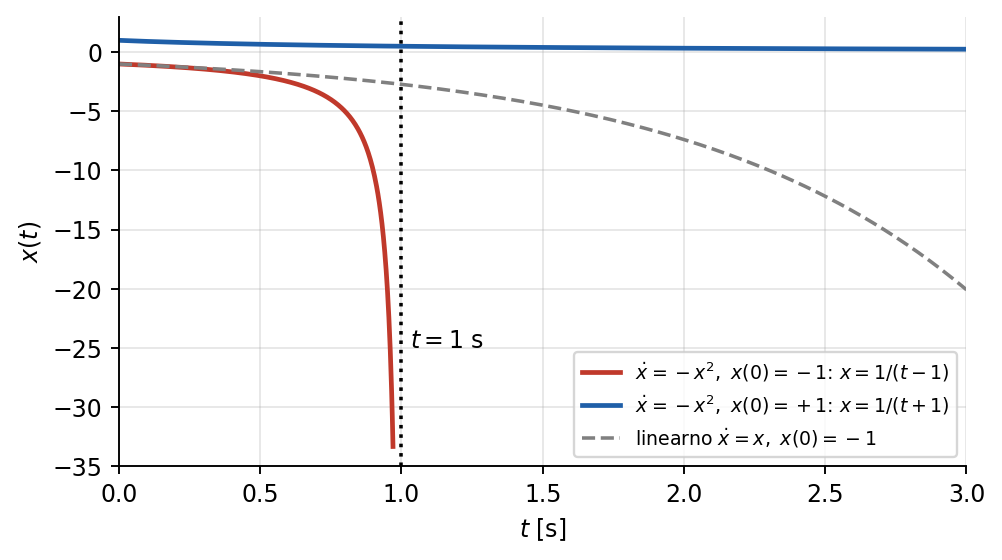
\includegraphics[width=0.7\linewidth,height=\textheight,keepaspectratio,alt={Konačno vreme bekstva: isti sistem ẋ = -x² iz x(0) = -1 ode u -∞ za 1 s, a iz x(0) = +1 mirno teži nuli; linearni nestabilni sistem (isprekidano) raste bez granice, ali tek kad t → ∞}]{figures/nel_finite_escape.png}
\caption{Konačno vreme bekstva: isti sistem ẋ = -x² iz x(0) = -1 ode u -∞ za 1 s, a iz x(0) = +1 mirno teži nuli; linearni nestabilni sistem (isprekidano) raste bez granice, ali tek kad t → ∞}
\end{figure}

Zašto se to dešava: brzina rasta \(|\dot x| = x^2\) raste brže od samog \(|x|\). Vreme potrebno da se stigne do beskonačnosti je \(\int^{\infty} dx/x^2\), a taj integral je \textbf{konačan}. Kod linearnog \(\dot x = ax\) vreme je \(\int^\infty dx/(ax)\), a taj integral divergira. Iz \(x(0) = +1\) isti sistem daje \(x(t) = 1/(t + 1) \to 0\): ishod zavisi od početnog uslova.

U domaćem se ova pojava vidi u zadatku 2.3 (Khalil 7.11 pod 1, nelinearnost \(y^5\)): iz početnog stanja iznad nestabilnog ciklusa rešenje eksplodira za oko 0,1 s.

\subsubsection{3. Više izolovanih tačaka ravnoteže}

Za iste parametre sistem može završiti u različitim stanjima, zavisno od početnog uslova. Primer je klatno (ispod) i domaći 1.2 (dva čvora i dva sedla).

\subsubsection{\texorpdfstring{4. Granični ciklus (\emph{limit cycle})}{4. Granični ciklus (limit cycle)}}

Sistem trajno osciluje \textbf{istom amplitudom i periodom}, bez obzira na početno stanje (unutar oblasti privlačenja ciklusa). U faznoj ravni to je \textbf{izolovana zatvorena trajektorija}.

Linearni sistem ovo ne može:

\begin{itemize}
\item trajne oscilacije postoje samo za čisto imaginarne polove, a tada amplituda zavisi od početnog stanja;
\item najmanja promena parametra pomera polove sa imaginarne ose, pa oscilacije počnu da rastu ili da se guše.
\end{itemize}

Zato svaki stabilan oscilator (npr. u elektronici) mora biti nelinearan. Detaljno u poglavlju o faznoj ravni (Van der Pol).

\subsubsection{5. Jump fenomen}

Kod opruge sa nelinearnom krutošću amplituda prinudnih oscilacija \textbf{naglo skače} pri sporoj promeni frekvencije pobude (opisano ispod, kod opruge).

\subsection{Primeri}

\subsubsection{Klatno}

Nit dužine \(L\), masa \(m\), otklon \(\theta\) od vertikale. Po tangenti deluje komponenta težine \(-mg\sin\theta\), pa drugi Njutnov zakon daje:

\[mL\ddot\theta = -mg\sin\theta \quad\Rightarrow\quad \ddot\theta = -\frac{g}{L}\sin\theta\]

Sa viskoznim trenjem (sila \(kL\dot\theta\), srazmerna brzini mase \(L\dot\theta\); njen moment je \(kL^2\dot\theta\)) i upravljačkim momentom \(T\), jednačina momenata oko tačke vešanja je \(mL^2\ddot\theta = -mgL\sin\theta - kL^2\dot\theta + T\). Deljenjem sa \(mL^2\):

\[\ddot\theta = -\frac{g}{L}\sin\theta - \frac{k}{m}\dot\theta + \frac{T}{mL^2}\]

Za malo \(\theta\) je \(\sin\theta \approx \theta\), pa se dobija linearni oscilator. On važi samo oko donjeg položaja.

\textbf{Tačke ravnoteže} (bez momenta, \(x_1 = \theta\), \(x_2 = \dot\theta\)):

\[\dot x_1 = x_2, \qquad \dot x_2 = -\frac{g}{L}\sin x_1 - \frac{k}{m}x_2\]

Iz \(\dot x_1 = 0\) sledi \(x_2 = 0\), a iz \(\dot x_2 = 0\) sledi \(\sin x_1 = 0\), tj. \(x_1 = k\pi\). Ima ih beskonačno mnogo, ali fizički samo dve: \textbf{dole} (\(0, 2\pi, \dots\)) i \textbf{gore} (\(\pi, 3\pi, \dots\)). Linearni model „vidi'' samo jednu od njih. Tip ovih tačaka određen je u poglavlju o faznoj ravni: dole je stabilan fokus, gore sedlo.

\subsubsection{Opruga: tvrda i meka}

Masa na opruzi, bez trenja, spoljašnja sila \(F\):

\[m\ddot x + F_{el}(x) = F, \qquad F_{el} = k(1 \pm a^2x^2)\,x \qquad (+\ \text{tvrda},\ -\ \text{meka})\]

Linearna opruga \(F_{el} = kx\) važi samo za male deformacije. Tvrda opruga sa istezanjem postaje sve kruća: \(m\ddot x + kx + ka^2x^3 = F\).

Linearni oscilator za svaku frekvenciju ima \textbf{jednu} amplitudu, sa rezonancom u \(\omega_n = \sqrt{k/m}\). Kod tvrde opruge efektivna krutost raste sa amplitudom, pa i rezonantna učestanost raste sa amplitudom. Vrh amplitudne karakteristike se zato „nagne'' udesno, i za neke frekvencije postoje \textbf{dve} stabilne amplitude:

\begin{itemize}
\item pri \textbf{povećanju} frekvencije amplituda prati gornju granu, pa u jednoj tački naglo padne na donju;
\item pri \textbf{smanjenju} frekvencije prati donju granu, pa naglo skoči na gornju.
\end{itemize}

To je \textbf{jump fenomen}. Srednja grana između tačaka skoka je nestabilna i ne vidi se u eksperimentu. Kod meke opruge kriva se naginje ulevo.

\subsection{Tipične nelinearnosti}

\begin{figure}
\centering
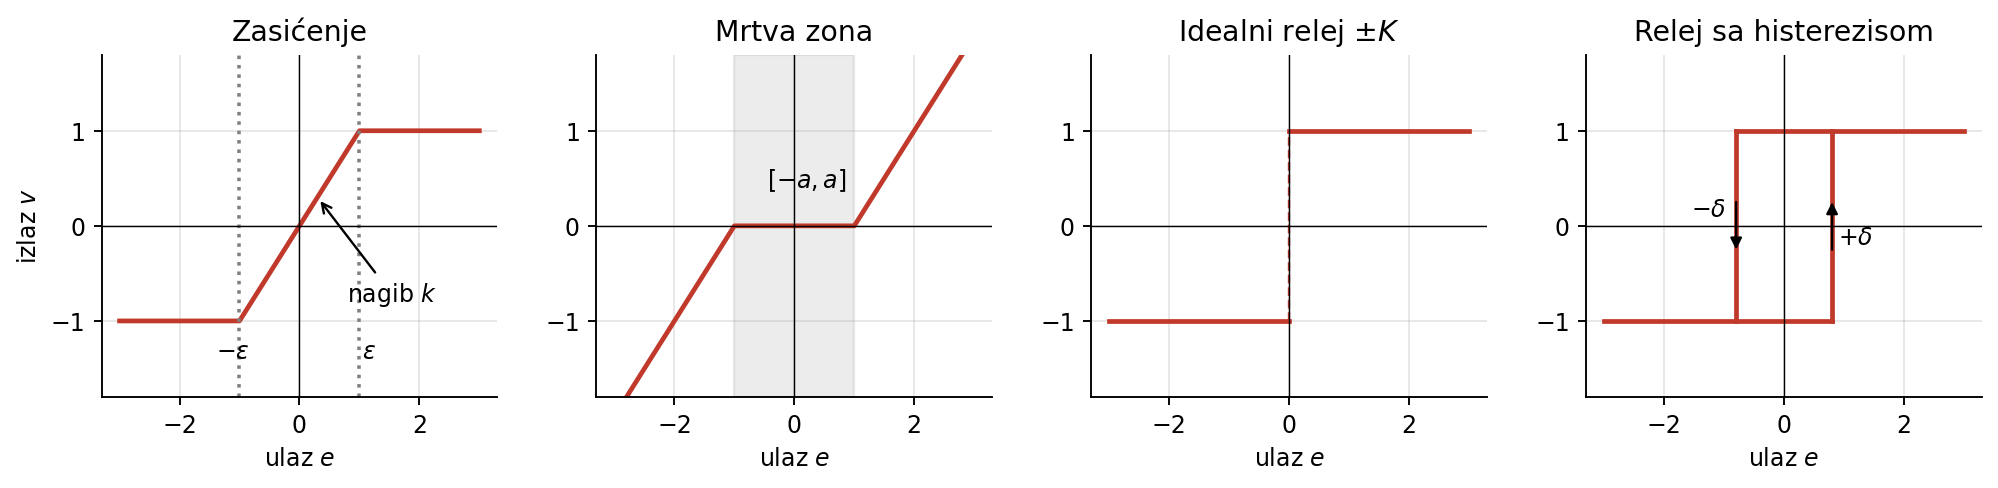
\includegraphics[width=0.95\linewidth,height=\textheight,keepaspectratio,alt={Tipične statičke nelinearnosti: zasićenje (linearno samo između -ε i ε), mrtva zona (izlaz nula za \textbar e\textbar{} \textless{} a), idealni relej i relej sa histerezisom (prebacuje se na +K tek kad ulaz poraste iznad +δ, a na -K kad padne ispod -δ)}]{figures/nel_nelinearnosti.png}
\caption{Tipične statičke nelinearnosti: zasićenje (linearno samo između -ε i ε), mrtva zona (izlaz nula za \textbar e\textbar{} \textless{} a), idealni relej i relej sa histerezisom (prebacuje se na +K tek kad ulaz poraste iznad +δ, a na -K kad padne ispod -δ)}
\end{figure}

\begin{itemize}
\item \textbf{Zasićenje (saturacija):} \(v = ke\) za \(|e| \le \varepsilon\), a \(v = k\varepsilon\operatorname{sign}(e)\) van toga. Svaki aktuator ima ograničen izlaz.
\item \textbf{Mrtva zona:} za \(|e| < a\) izlaz je 0 (npr. motor ne kreće dok napon ne savlada statičko trenje).
\item \textbf{Idealni relej:} \(v = K\operatorname{sign}(e)\).
\item \textbf{Relej sa histerezisom:} izlaz zavisi i od \textbf{smera} promene ulaza, pa je karakteristika zatvorena kontura, a ne kriva.
\item \textbf{Zazor (\emph{backlash}):} mehanički primer histerezisa sa predavanja. Na pogonskom disku je zub, a na gonjenom žleb širi od zuba. Pri promeni smera zub prvo pređe prazan hod, pa tek onda povuče drugi disk.
\end{itemize}

Sve ove nelinearnosti su \textbf{statičke} (izlaz ne zavisi od brzine promene ulaza, pa ni od frekvencije) i \textbf{neparne} (\(f(-e) = -f(e)\)). Histerezis i zazor imaju „memoriju'' (izlaz zavisi od smera promene), ali ne i od brzine, pa se i oni ubrajaju u statičke u ovom smislu. Obe osobine su važne za opisnu funkciju: statičnost daje \(N\) nezavisno od \(\omega\), a neparnost izlaz bez srednje vrednosti.

\begin{ispit}
Znati nabrojati pet pojava koje linearni sistem nema (superpozicija, konačno vreme bekstva, više ravnotežnih tačaka, granični ciklus, jump) i za svaku dati primer. Za konačno vreme bekstva ume se izvesti \(x(t) = 1/(t-1)\) za \(\dot x = -x^2\), \(x(0) = -1\). Česta greška: reći da \(x \to +\infty\); tačno je \(x \to -\infty\) kada \(t \to 1^-\).
\end{ispit}

\section{Fazna ravan}

\subsection{Ideja}

Sistem drugog reda \(\dot x_1 = f_1(x_1, x_2)\), \(\dot x_2 = f_2(x_1, x_2)\) može se nacrtati kao kretanje tačke u ravni \((x_1, x_2)\). Vreme se ne vidi, ali se na jednoj slici vidi ponašanje iz \textbf{svih} početnih stanja: gde su ravnoteže, koje su stabilne, odakle se ide u beskonačnost i da li postoji oscilacija. Postupak je uvek isti: nađu se tačke ravnoteže, oko svake se sistem linearizuje, tip tačke se pročita iz svojstvenih vrednosti, pa se lokalne slike spoje u globalni portret.

\subsection{Fazna ravan, vektorsko polje, fazni portret}

\begin{itemize}
\item \textbf{Trajektorija}: kriva koju opisuje \((x_1(t), x_2(t))\) za jedno početno stanje. Informacija o vremenu se gubi, pa je prikaz kvalitativan.
\item \textbf{Zatvorena} trajektorija znači periodično kretanje; \textbf{otvorena} znači aperiodično.
\item \textbf{Vektorsko polje}: u svakoj tački vektor \(f(x) = [f_1, f_2]^T\) je tangenta na trajektoriju kroz tu tačku. Primer sa predavanja: za \(f = [2x_1^2,\ x_2]^T\) u tački \((1, 1)\) vektor je \([2, 1]^T\).
\item \textbf{Fazni portret}: familija trajektorija za različita početna stanja.
\end{itemize}

Trajektorije autonomnog sistema \textbf{ne mogu da se seku} (kroz svaku tačku prolazi tačno jedna, jer je \(f(x)\) jednoznačno). Zato portret u ravni ima jednostavnu strukturu: ograničena trajektorija u ravni može samo da završi u ravnoteži ili na zatvorenoj trajektoriji (posledica teoreme Poenkare--Bendikson, niže). Zato u ravni nema haosa; on je moguć tek od trećeg reda.

U Matlabu: vektorsko polje se crta sa \texttt{quiver} ili \texttt{streamslice} (strelice pokazuju smer), a pojedinačne trajektorije sa \texttt{ode45} iz više početnih tačaka \izvor{\texttt{pomocne/\allowbreak{}fazni\_\allowbreak{}portret.m}}.

\subsection{Fazni portreti linearnih sistema}

\subsubsection{Modalne koordinate}

Za \(\dot x = Ax\) uvodimo nove koordinate \(z\) preko \(x = Pz\), gde su kolone matrice \(P\) svojstveni vektori:

\[P\dot z = APz \quad\Rightarrow\quad \dot z = P^{-1}AP\,z = \Lambda z\]

Zašto baš svojstveni vektori: iz \(Av_i = \lambda_iv_i\) za sve kolone odjednom sledi \(AP = P\Lambda\), tj. \(P^{-1}AP = \Lambda\) je dijagonalna (kada su \(\lambda_i\) realne i različite).

\(\Lambda\) je \textbf{realna Žordanova forma}. Za sistem drugog reda ima tri oblika:

\begin{longtable}[]{@{}
  >{\raggedright\arraybackslash}p{(\linewidth - 2\tabcolsep) * \real{0.4444}}
  >{\centering\arraybackslash}p{(\linewidth - 2\tabcolsep) * \real{0.5556}}@{}}
\caption{Realna Žordanova forma za sistem drugog reda}\tabularnewline
\toprule\noalign{}
\begin{minipage}[b]{\linewidth}\raggedright
Svojstvene vrednosti
\end{minipage} & \begin{minipage}[b]{\linewidth}\centering
\(\Lambda\)
\end{minipage} \\
\midrule\noalign{}
\endfirsthead
\toprule\noalign{}
\begin{minipage}[b]{\linewidth}\raggedright
Svojstvene vrednosti
\end{minipage} & \begin{minipage}[b]{\linewidth}\centering
\(\Lambda\)
\end{minipage} \\
\midrule\noalign{}
\endhead
\bottomrule\noalign{}
\endlastfoot
realne, različite \(\lambda_1 \ne \lambda_2\) & \(\begin{bmatrix}\lambda_1 & 0\\ 0 & \lambda_2\end{bmatrix}\) \\
realne, jednake \(\lambda_1 = \lambda_2 = \lambda\) & \(\begin{bmatrix}\lambda & 1\\ 0 & \lambda\end{bmatrix}\) \\
konjugovano kompleksne \(\alpha \pm j\beta\) & \(\begin{bmatrix}\alpha & -\beta\\ \beta & \alpha\end{bmatrix}\) \\
\end{longtable}

Za jednake svojstvene vrednosti druga kolona \(P\) je generalisani svojstveni vektor (\((A - \lambda I)v_2 = v_1\)). Za kompleksne se uzima \(P = [v_r\ \ v_i]\), realni i imaginarni deo svojstvenog vektora. Svojstvene vrednosti su \textbf{invarijante}: ne zavise od izbora koordinata.

Primer: \(A = \begin{bmatrix}0 & 1\\ 8 & -2\end{bmatrix}\) daje \(\det(\lambda I - A) = \lambda^2 + 2\lambda - 8 = 0\), pa je \(\lambda_1 = -4\), \(\lambda_2 = 2\), sa \(v_1 = [1, -4]^T\) i \(v_2 = [1, 2]^T\). U modalnim koordinatama \(\dot z_1 = -4z_1\), \(\dot z_2 = 2z_2\): jednačine su raspregnute. (Česta greška pri prepisivanju: \(\lambda^2 - 2\lambda - 6\); tačno je \(\lambda^2 + 2\lambda - 8\).)

\subsubsection{Slučaj 1: realne i različite svojstvene vrednosti}

Svaka jednačina se reši posebno: \(z_1(t) = z_{10}e^{\lambda_1 t}\), \(z_2(t) = z_{20}e^{\lambda_2 t}\). Eliminišemo vreme. Iz prve je \(e^{\lambda_1 t} = z_1/z_{10}\), a

\[e^{\lambda_2 t} = \left(e^{\lambda_1 t}\right)^{\lambda_2/\lambda_1} = \left(\frac{z_1}{z_{10}}\right)^{\lambda_2/\lambda_1} \quad\Rightarrow\quad z_2 = c\, z_1^{\lambda_2/\lambda_1}, \qquad c = \frac{z_{20}}{z_{10}^{\lambda_2/\lambda_1}}\]

\begin{itemize}
\item \textbf{Obe negativne} (\(\lambda_2 < \lambda_1 < 0\)): eksponent \(\lambda_2/\lambda_1 > 1\), obe koordinate opadaju. Nagib \(dz_2/dz_1 \sim z_1^{\lambda_2/\lambda_1 - 1} \to 0\) kada \(z_1 \to 0\), pa trajektorije ulaze u tačku \textbf{tangentno na sporiji svojstveni vektor} \(v_1\) (onaj sa manjim \(|\lambda|\)). To je \textbf{stabilan čvor}.
\item \textbf{Obe pozitivne}: iste krive, strelice suprotno. \textbf{Nestabilan čvor}.
\item \textbf{Različitog znaka} (\(\lambda_2 < 0 < \lambda_1\)): eksponent je negativan, krive su „hiperbole''. U tačku se ulazi samo duž stabilnog svojstvenog vektora, a izlazi duž nestabilnog. To je \textbf{sedlo} (uvek nestabilno).
\end{itemize}

\subsubsection{Slučaj 2: kompleksne svojstvene vrednosti α ± jβ}

\[\dot z_1 = \alpha z_1 - \beta z_2, \qquad \dot z_2 = \beta z_1 + \alpha z_2\]

Jednačine su spregnute, pa prelazimo u polarne koordinate \(z_1 = r\cos\theta\), \(z_2 = r\sin\theta\). Iz \(r^2 = z_1^2 + z_2^2\) diferenciranjem:

\[r\dot r = z_1\dot z_1 + z_2\dot z_2 = \alpha z_1^2 - \beta z_1z_2 + \beta z_1 z_2 + \alpha z_2^2 = \alpha r^2 \quad\Rightarrow\quad \dot r = \alpha r\]

Iz \(\operatorname{tg}\theta = z_2/z_1\) dobija se \(\dot\theta = (z_1\dot z_2 - z_2\dot z_1)/r^2\):

\[\dot\theta = \frac{\beta z_1^2 + \alpha z_1z_2 - \alpha z_1 z_2 + \beta z_2^2}{r^2} = \beta\]

Dakle \(r(t) = r_0e^{\alpha t}\) i \(\theta(t) = \theta_0 + \beta t\): tačka kruži konstantnom ugaonom brzinom, a poluprečnik se eksponencijalno menja. (Isto se dobija eliminacijom iz dve jednačine za \(\dot z_1\), \(\dot z_2\).)

\begin{itemize}
\item \(\alpha < 0\): spirala ka tački, \textbf{stabilan fokus}.
\item \(\alpha > 0\): spirala od tačke, \textbf{nestabilan fokus}.
\item \(\alpha = 0\): zatvorene krive (elipse u \(x\)), \textbf{centar}. Amplituda zavisi od početnog stanja.
\end{itemize}

\subsubsection{Slučaj 3: jednake i nulte svojstvene vrednosti}

\begin{itemize}
\item \(\lambda_1 = \lambda_2 = \lambda \ne 0\) sa jednim svojstvenim vektorom: \(z_2 = z_{20}e^{\lambda t}\), \(z_1 = (z_{10} + z_{20}t)e^{\lambda t}\). Dobija se \textbf{degenerisan čvor}: sve trajektorije ulaze (ili izlaze) tangentno na jedan pravac.
\item Jedna svojstvena vrednost nula (\(\lambda_1 = 0\)): \(z_1 = z_{10}\) je konstantno, pa je cela prava \(z_2 = 0\) skup ravnotežnih tačaka. Trajektorije su prave paralelne sa \(v_2\), ka toj pravoj ako je \(\lambda_2 < 0\). Ovaj slučaj se javlja u domaćem 3.2 (nulta dinamika sistema 2).
\end{itemize}

\begin{figure}
\centering
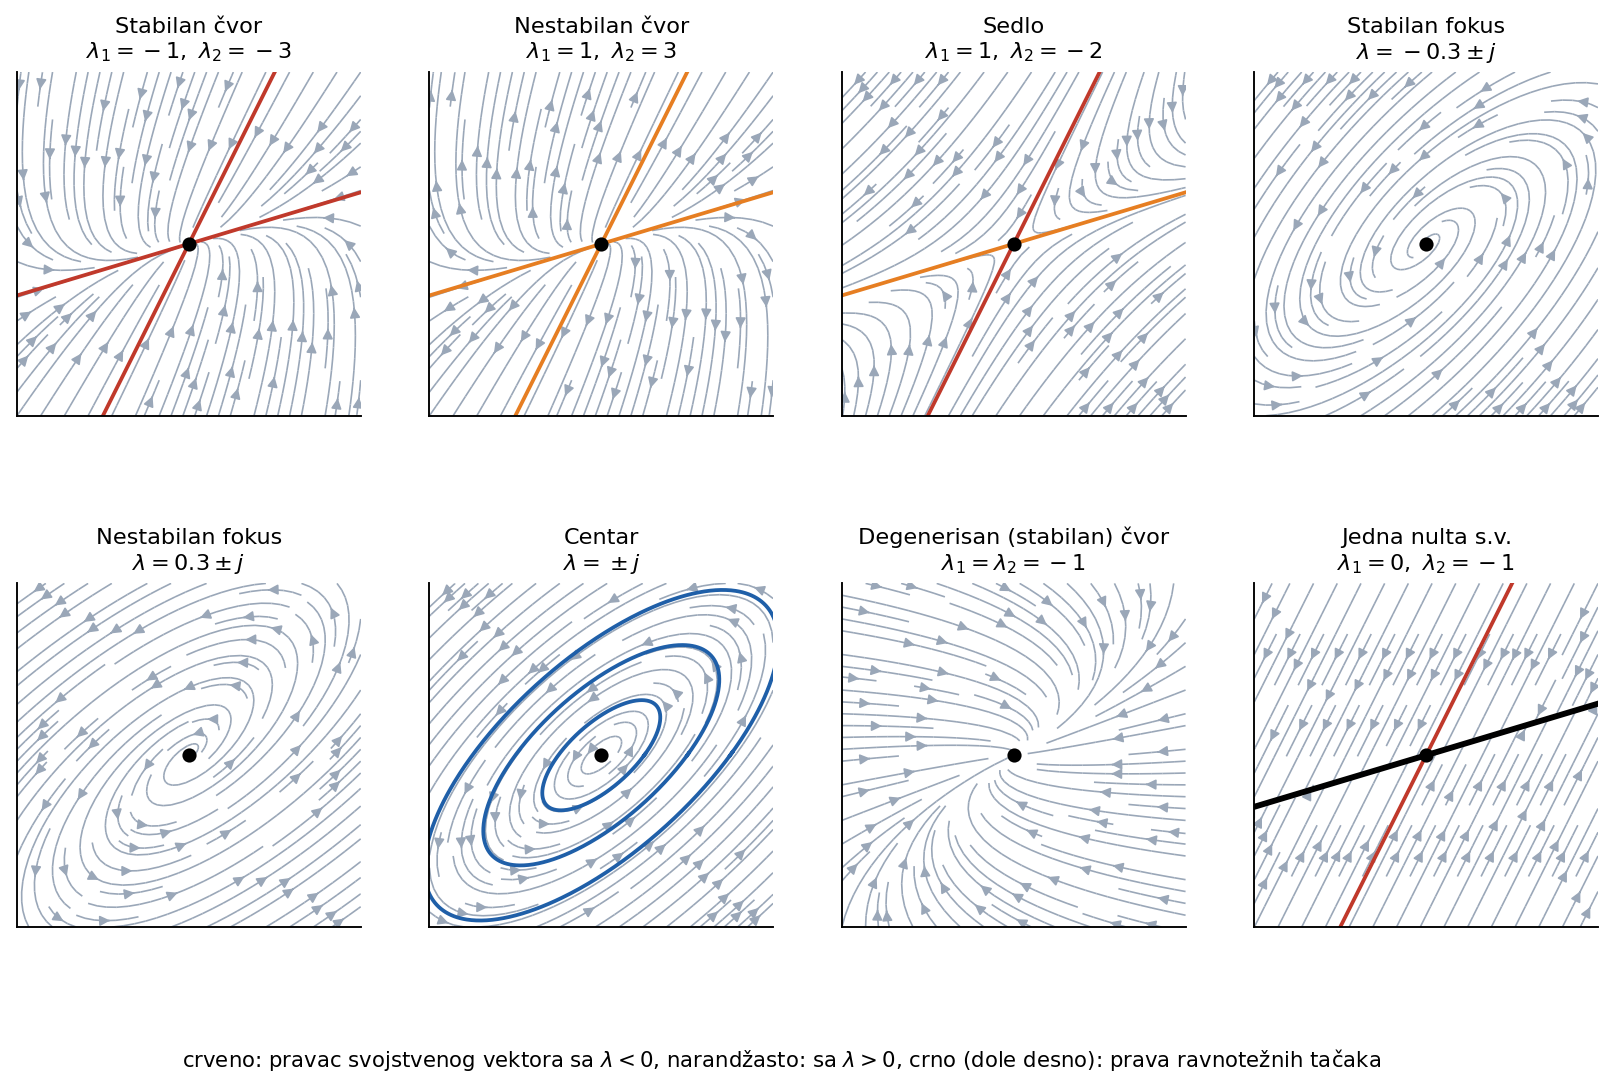
\includegraphics[width=1\linewidth,height=\textheight,keepaspectratio,alt={Svi tipovi singularnih tačaka linearnog sistema drugog reda. Kod čvorova i sedla vide se pravci svojstvenih vektora (crveno za λ \textless{} 0, narandžasto za λ \textgreater{} 0); kod stabilnog čvora trajektorije ulaze tangentno na sporiji pravac; kod centra amplituda zavisi od početnog stanja; kod nulte svojstvene vrednosti postoji cela prava ravnotežnih tačaka}]{figures/nel_singularne_tacke.png}
\caption{Svi tipovi singularnih tačaka linearnog sistema drugog reda. Kod čvorova i sedla vide se pravci svojstvenih vektora (crveno za λ \textless{} 0, narandžasto za λ \textgreater{} 0); kod stabilnog čvora trajektorije ulaze tangentno na sporiji pravac; kod centra amplituda zavisi od početnog stanja; kod nulte svojstvene vrednosti postoji cela prava ravnotežnih tačaka}
\end{figure}

\subsubsection{Brza klasifikacija: trag i determinanta}

Karakteristični polinom matrice \(2 \times 2\) zavisi samo od traga \(\tau = \operatorname{tr}A = \lambda_1 + \lambda_2\) i determinante \(\Delta = \det A = \lambda_1\lambda_2\):

\[\lambda^2 - \tau\lambda + \Delta = 0, \qquad \lambda_{1,2} = \frac{\tau \pm \sqrt{\tau^2 - 4\Delta}}{2}\]

Iz toga se tip čita bez računanja korena:

\begin{itemize}
\item \(\Delta < 0\): koreni realni i suprotnog znaka, \textbf{sedlo};
\item \(\Delta > 0\) i \(\tau^2 > 4\Delta\): realni, istog znaka, \textbf{čvor} (stabilan za \(\tau < 0\));
\item \(\Delta > 0\) i \(\tau^2 < 4\Delta\): kompleksni, \textbf{fokus} (stabilan za \(\tau < 0\));
\item \(\Delta > 0\) i \(\tau = 0\): \textbf{centar};
\item \(\tau^2 = 4\Delta\): dvostruka svojstvena vrednost, degenerisan čvor;
\item \(\Delta = 0\): bar jedna svojstvena vrednost je nula, pa postoji cela prava ravnoteža (slučaj 3).
\end{itemize}

\begin{figure}
\centering
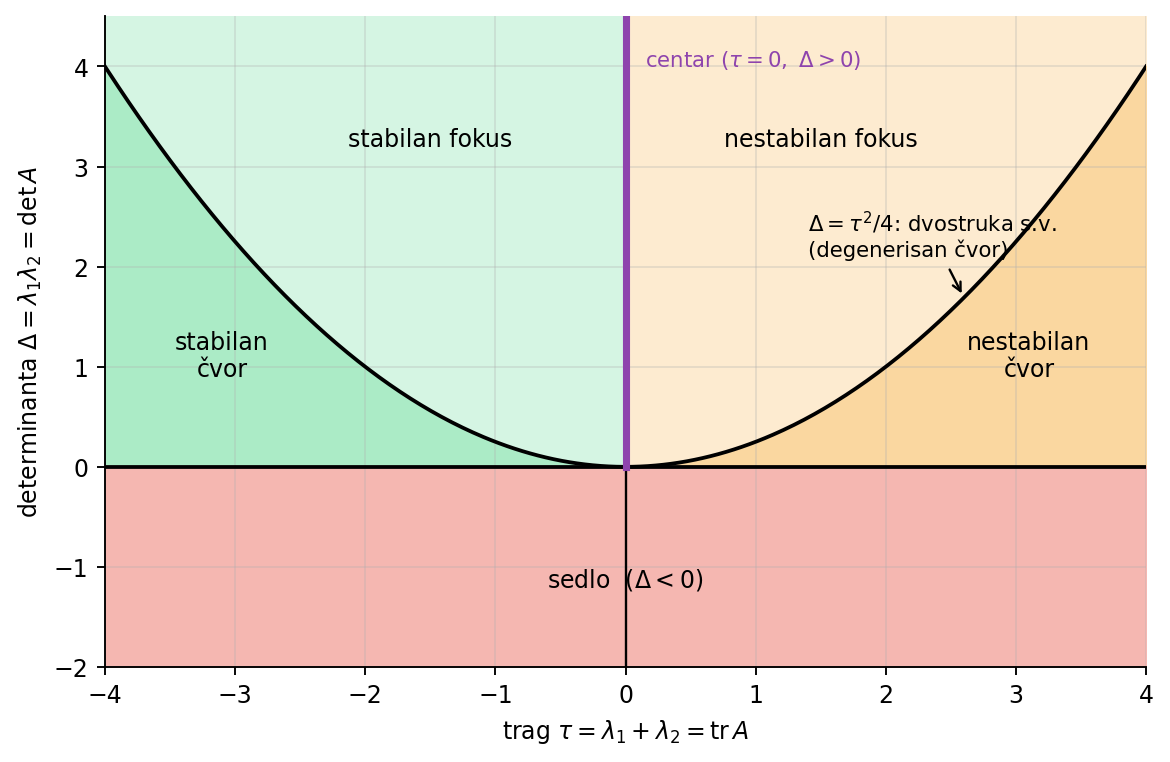
\includegraphics[width=0.7\linewidth,height=\textheight,keepaspectratio,alt={Ravan trag--determinanta: ispod ose Δ = 0 su sedla, iznad parabole Δ = τ²/4 fokusi, između nje i ose čvorovi; leva polovina je stabilna, desna nestabilna, a pozitivna Δ-osa su centri}]{figures/nel_trag_det.png}
\caption{Ravan trag--determinanta: ispod ose Δ = 0 su sedla, iznad parabole Δ = τ²/4 fokusi, između nje i ose čvorovi; leva polovina je stabilna, desna nestabilna, a pozitivna Δ-osa su centri}
\end{figure}

\subsection{Linearizacija nelinearnog sistema}

\subsubsection{Jakobijan}

Neka je \(p = (p_1, p_2)\) tačka ravnoteže, \(f(p) = 0\). Razvoj u Tejlorov red oko \(p\):

\[\dot x_i = \underbrace{f_i(p)}_{=0} + \frac{\partial f_i}{\partial x_1}\Big|_p (x_1 - p_1) + \frac{\partial f_i}{\partial x_2}\Big|_p (x_2 - p_2) + \text{članovi višeg reda}\]

Sa odstupanjem \(y = x - p\) (pa je \(\dot y = \dot x\)) i zanemarenim višim članovima:

\[\dot y = Jy, \qquad J = \frac{\partial f}{\partial x}\Big|_{x = p} = \begin{bmatrix} \dfrac{\partial f_1}{\partial x_1} & \dfrac{\partial f_1}{\partial x_2} \\ \dfrac{\partial f_2}{\partial x_1} & \dfrac{\partial f_2}{\partial x_2} \end{bmatrix}_{x = p}\]

\subsubsection{Kada linearizacija daje tačan zaključak}

Na predavanju je dat argument perturbacija: nelinearni članovi se ponašaju kao mala promena matrice, \(J + \Delta J\). Svojstvene vrednosti zavise neprekidno od elemenata matrice, pa za dovoljno malo \(\Delta J\) ostaju u malom krugu oko svojstvenih vrednosti od \(J\).

\begin{itemize}
\item Ako je \(\operatorname{Re}\lambda \ne 0\) (čvor, sedlo, fokus), mali pomeraj ne menja znak realnog dela, pa se tip \textbf{ne menja}.
\item Kod \textbf{centra} je \(\operatorname{Re}\lambda = 0\), i najmanji pomeraj ga pretvara u stabilan ili nestabilan fokus. Centar je „strukturno nestabilan''.
\end{itemize}

To je sadržaj teoreme Hartman--Grobman \izvor{standardna teorija, Khalil 2.3}: ako Jakobijan nema svojstvenih vrednosti sa nultim realnim delom (tačka je \textbf{hiperbolična}), fazni portret nelinearnog sistema u \textbf{maloj okolini} tačke kvalitativno je isti kao portret linearizacije.

Primer da centar ne važi \izvor{standardna teorija, Khalil odelj. 2.3}: sistem

\[\dot x_1 = -x_2 - \mu x_1(x_1^2 + x_2^2), \qquad \dot x_2 = x_1 - \mu x_2(x_1^2 + x_2^2)\]

ima Jakobijan u nuli \(\begin{bmatrix}0 & -1\\ 1 & 0\end{bmatrix}\), tj. centar. U polarnim koordinatama, istim računom kao gore, dobija se \(\dot r = -\mu r^3\), \(\dot\theta = 1\). Za \(\mu > 0\) tačka je stabilan fokus, a za \(\mu < 0\) nestabilan. Linearizacija to ne vidi.

\begin{zasto}
Linearizacija daje samo \textbf{lokalnu} sliku. Ona ne kaže koliko je velika oblast privlačenja, niti da li postoje druge ravnoteže ili granični ciklusi. Zato se posle lokalne analize crta ceo portret (primer: domaći 1.3).
\end{zasto}

\subsubsection{Primer: klatno sa trenjem}

Sa \(g/L = 10\) i \(k/m = 1\):

\[\dot x_1 = x_2, \qquad \dot x_2 = -10\sin x_1 - x_2, \qquad J = \begin{bmatrix} 0 & 1\\ -10\cos x_1 & -1\end{bmatrix}\]

\begin{itemize}
\item \((0, 0)\): \(J = \begin{bmatrix}0 & 1\\ -10 & -1\end{bmatrix}\), \(\lambda^2 + \lambda + 10 = 0\), \(\lambda = -0{,}5 \pm j3{,}12\). \textbf{Stabilan fokus}: klatno oscilujući stane dole.
\item \((\pi, 0)\): \(J = \begin{bmatrix}0 & 1\\ 10 & -1\end{bmatrix}\), \(\lambda^2 + \lambda - 10 = 0\), \(\lambda = 2{,}70\) i \(-3{,}70\). \textbf{Sedlo}: gornji položaj je nestabilan.
\end{itemize}

Po tragu i determinanti: u \((0,0)\) je \(\Delta = 10 > 0\), \(\tau = -1\), \(\tau^2 < 4\Delta\), pa je stabilan fokus; u \((\pi, 0)\) je \(\Delta = -10 < 0\), pa je sedlo.

\begin{figure}
\centering
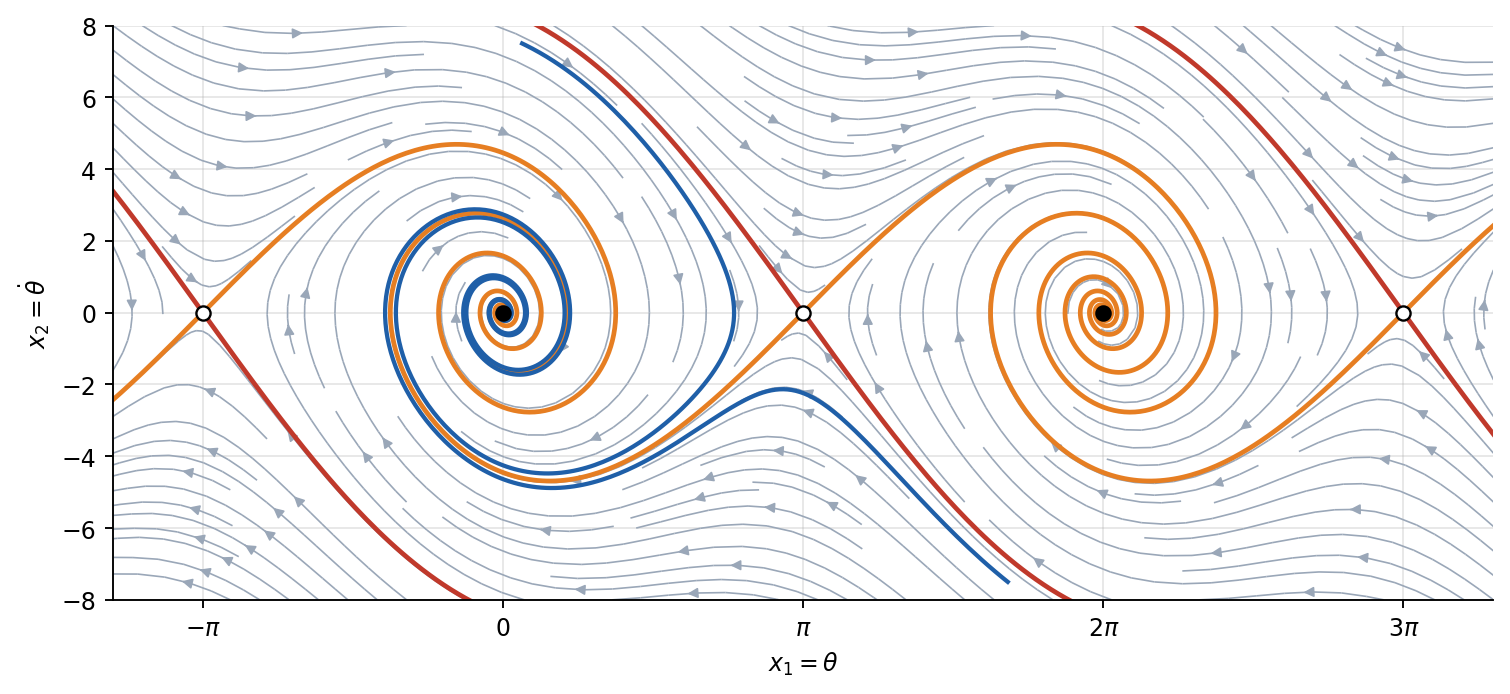
\includegraphics[width=0.95\linewidth,height=\textheight,keepaspectratio,alt={Fazni portret klatna sa trenjem: puni krugovi su stabilni fokusi (donji položaj), prazni su sedla (gornji položaj); stabilne separatrise sedala dele ravan na oblasti koje završavaju u različitim donjim ravnotežama (klatno napravi ceo krug ili ne)}]{figures/nel_klatno.png}
\caption{Fazni portret klatna sa trenjem: puni krugovi su stabilni fokusi (donji položaj), prazni su sedla (gornji položaj); stabilne separatrise sedala dele ravan na oblasti koje završavaju u različitim donjim ravnotežama (klatno napravi ceo krug ili ne)}
\end{figure}

\subsection{Postupak crtanja faznog portreta}

Ovaj postupak se traži u domaćim zadacima 1.1--1.3:

\begin{enumerate}
\def\labelenumi{\arabic{enumi}.}
\item \textbf{Tačke ravnoteže}: rešiti \(f_1 = 0\), \(f_2 = 0\).
\item \textbf{Jakobijan} u opštem obliku, pa u svakoj tački.
\item \textbf{Tip} svake tačke iz svojstvenih vrednosti (ili iz \(\tau\) i \(\Delta\)).
\item Za \textbf{sedla} izračunati svojstvene vektore: to su pravci \textbf{separatrisa}. Separatrise su četiri posebne trajektorije sedla: dve koje ulaze u sedlo (stabilne, duž svojstvenog vektora sa \(\lambda < 0\)) i dve koje iz njega izlaze (nestabilne, duž vektora sa \(\lambda > 0\)). Stabilne separatrise dele ravan na oblasti sa različitim konačnim ponašanjem, pa su granice oblasti privlačenja.
\item Za čvorove izračunati sporiji svojstveni vektor (pravac ulaska trajektorija). Za fokuse odrediti smer obrtanja (npr. znak \(\dot x_1\) u gornjoj poluravni).
\item \textbf{Globalno ponašanje}: šta rade trajektorije daleko od ravnoteža (koji član dominira za veliko \(|x|\)), da li postoji granični ciklus.
\item U Matlabu: vektorsko polje + trajektorije. Separatrise se dobijaju integracijom iz tačke malo pomerene od sedla duž svojstvenog vektora: \textbf{unazad} u vremenu za stabilnu, \textbf{unapred} za nestabilnu. Zašto unazad: stabilna separatrisa ulazi u sedlo, pa se integracijom unapred nikad ne bi pogodila tačno (najmanja greška početnog stanja odvede trajektoriju duž nestabilnog pravca). U obrnutom vremenu sedlo zameni uloge pravaca, pa ista kriva postane „privlačna'' i numerički se lako prati.
\end{enumerate}

\subsection{Granični ciklusi}

\subsubsection{Definicija i vrste}

\textbf{Granični ciklus} je izolovana zatvorena trajektorija: u njenoj okolini nema drugih zatvorenih trajektorija (za razliku od centra, gde su sve susedne trajektorije takođe zatvorene).

\begin{itemize}
\item \textbf{Stabilan}: susedne trajektorije se sa obe strane približavaju ciklusu.
\item \textbf{Nestabilan}: sa obe strane se udaljavaju.
\item \textbf{Polustabilan}: sa jedne strane se približavaju, a sa druge udaljavaju.
\end{itemize}

\subsubsection{Primer u polarnim koordinatama}

\[\dot x_1 = x_2 + x_1(1 - x_1^2 - x_2^2), \qquad \dot x_2 = -x_1 + x_2(1 - x_1^2 - x_2^2)\]

Sa \(r^2 = x_1^2 + x_2^2\) je \(r\dot r = x_1\dot x_1 + x_2\dot x_2\):

\[r\dot r = x_1x_2 + x_1^2(1 - r^2) - x_1x_2 + x_2^2(1 - r^2) = r^2(1 - r^2) \quad\Rightarrow\quad \dot r = r(1 - r^2)\]

\[\dot\theta = \frac{x_1\dot x_2 - x_2\dot x_1}{r^2} = \frac{-x_1^2 + x_1x_2(1 - r^2) - x_2^2 - x_1x_2(1 - r^2)}{r^2} = -1\]

Sada je sve jasno iz jednodimenzionalne jednačine za \(r\):

\begin{itemize}
\item \(\dot r = 0\) za \(r = 0\) i \(r = 1\);
\item za \(0 < r < 1\) je \(\dot r > 0\) (poluprečnik raste), a za \(r > 1\) je \(\dot r < 0\) (opada);
\item dakle krug \(r = 1\) je \textbf{stabilan granični ciklus}, a nula je nestabilna. Obrtanje je u smeru kazaljke na satu (\(\dot\theta = -1\)).
\end{itemize}

\begin{figure}
\centering
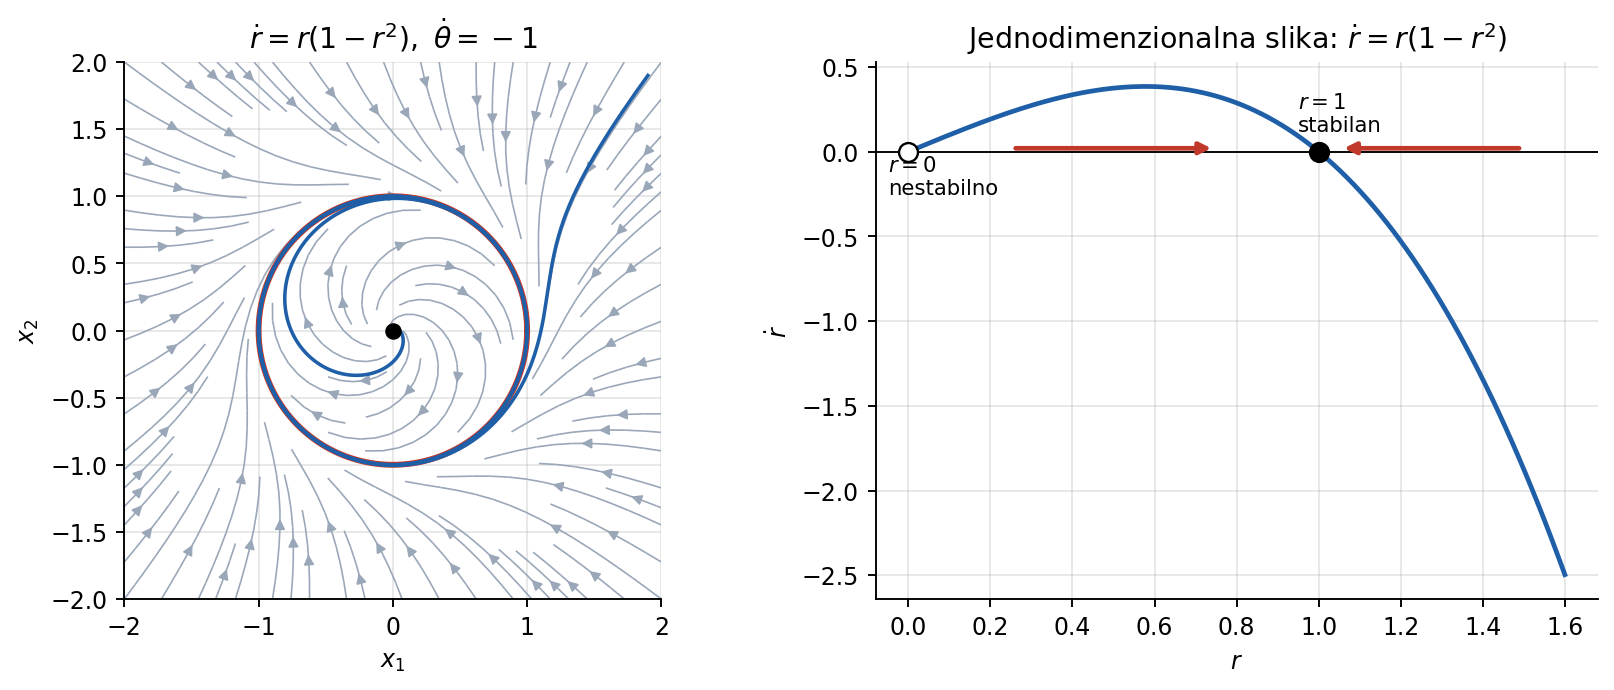
\includegraphics[width=0.9\linewidth,height=\textheight,keepaspectratio,alt={Levo: sve trajektorije, i iznutra i spolja, završe na jediničnom krugu. Desno: znak ṙ = r(1 - r²) pokazuje zašto: strelice na r-osi vode ka r = 1 sa obe strane}]{figures/nel_polarni_ciklus.png}
\caption{Levo: sve trajektorije, i iznutra i spolja, završe na jediničnom krugu. Desno: znak ṙ = r(1 - r²) pokazuje zašto: strelice na r-osi vode ka r = 1 sa obe strane}
\end{figure}

\subsubsection{Kako se dokazuje postojanje ciklusa}

Kad prelazak u polarne koordinate ne daje ovako čistu jednačinu, koriste se dva standardna rezultata \izvor{standardna teorija, Khalil 2.6}.

\textbf{Poenkare--Bendikson.} Neka je \(M\) zatvoren i ograničen skup u ravni koji je \textbf{pozitivno invarijantan} (trajektorija koja uđe ne izlazi) i ne sadrži tačke ravnoteže, ili sadrži samo jednu, nestabilan čvor ili fokus. Tada \(M\) sadrži periodičnu trajektoriju. U praksi se \(M\) pravi kao \textbf{prsten}: na unutrašnjoj granici trajektorije idu napolje, a na spoljašnjoj unutra. To se proverava preko znaka \(\dot V\) za \(V = x_1^2 + x_2^2\) (domaći 1.1).

\textbf{Bendiksonov kriterijum.} Ako divergencija

\[\operatorname{div} f = \frac{\partial f_1}{\partial x_1} + \frac{\partial f_2}{\partial x_2}\]

u jednostruko povezanoj oblasti \(D\) ne menja znak i nije identički nula, u \(D\) \textbf{nema} periodičnih trajektorija. Kriterijum služi da se ciklus \textbf{isključi}.

\subsubsection{Van der Pol oscilator}

Primer sa predavanja:

\[\dot x_1 = x_2, \qquad \dot x_2 = -x_1 + \varepsilon(1 - x_1^2)x_2, \qquad \varepsilon > 0\]

Član \(\varepsilon(1 - x_1^2)x_2\) je nelinearno „prigušenje'': za \(|x_1| < 1\) je negativno (dodaje energiju), a za \(|x_1| > 1\) pozitivno (troši energiju). Male oscilacije zato rastu, velike se guše, i ustaljuje se jedna amplituda.

Linearizacija u nuli: \(J = \begin{bmatrix}0 & 1\\ -1 & \varepsilon\end{bmatrix}\), pa je \(\tau = \varepsilon > 0\) i \(\Delta = 1\). Za \(0 < \varepsilon < 2\) je \(\tau^2 < 4\Delta\), pa je nula \textbf{nestabilan fokus}. Jedina ravnoteža je nestabilna, a trajektorije daleko od nule se vraćaju (za \(|x_1| > 1\) „prigušenje'' je pozitivno i troši energiju); zato, po Poenkare--Bendiksonu, postoji granični ciklus, a simulacija pokazuje da je stabilan.

\begin{figure}
\centering
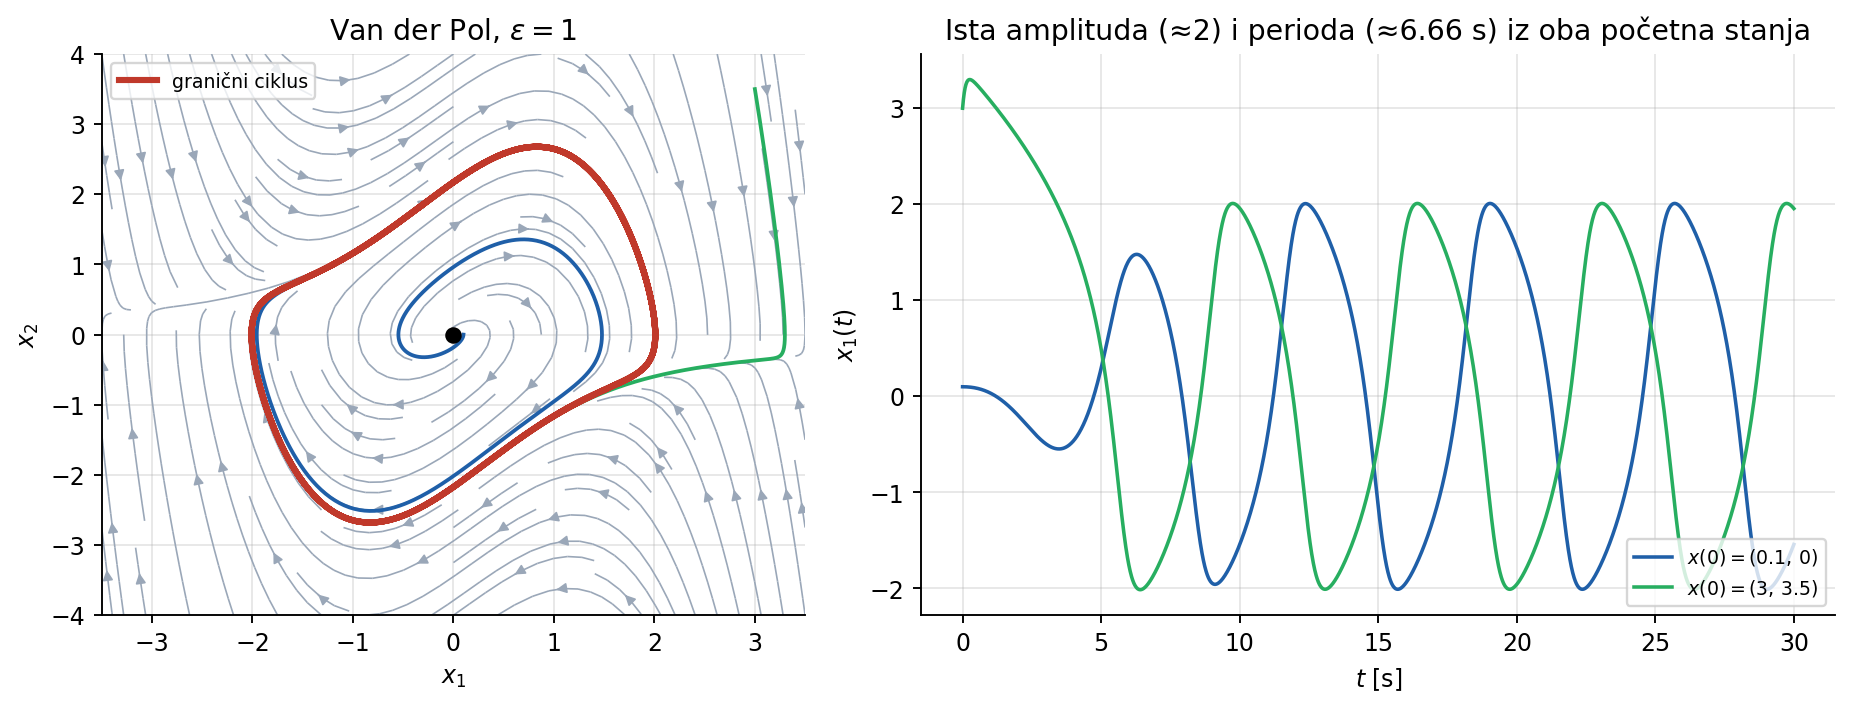
\includegraphics[width=0.95\linewidth,height=\textheight,keepaspectratio,alt={Van der Pol za ε = 1: trajektorija iz blizine nule se odmotava, a trajektorija spolja se namotava, i obe završe na istom ciklusu (crveno); desno se vidi da je ustaljena amplituda oko 2 i perioda oko 6,66 s, nezavisno od početnog stanja}]{figures/nel_vanderpol.png}
\caption{Van der Pol za ε = 1: trajektorija iz blizine nule se odmotava, a trajektorija spolja se namotava, i obe završe na istom ciklusu (crveno); desno se vidi da je ustaljena amplituda oko 2 i perioda oko 6,66 s, nezavisno od početnog stanja}
\end{figure}

\subsection{Domaći 1.1: Khalil 2.4 pod 3}

\[\dot x_1 = x_2, \qquad \dot x_2 = -x_1 + x_2(1 - 3x_1^2 - 2x_2^2)\]

\textbf{Ravnoteža.} Iz \(\dot x_1 = 0\) sledi \(x_2 = 0\), pa iz \(\dot x_2 = 0\) sledi \(x_1 = 0\). Jedina tačka je \((0, 0)\).

\textbf{Jakobijan.} Izvod \(x_2(1 - 3x_1^2 - 2x_2^2) = x_2 - 3x_1^2x_2 - 2x_2^3\) po \(x_1\) je \(-6x_1x_2\), a po \(x_2\) je \(1 - 3x_1^2 - 6x_2^2\):

\[J = \begin{bmatrix} 0 & 1\\ -1 - 6x_1x_2 & 1 - 3x_1^2 - 6x_2^2\end{bmatrix}, \qquad J(0,0) = \begin{bmatrix}0 & 1\\ -1 & 1\end{bmatrix}\]

\(\lambda^2 - \lambda + 1 = 0\), pa je \(\lambda = 0{,}5 \pm j0{,}866\): \textbf{nestabilan fokus}.

\textbf{Granični ciklus.} Uzmimo \(V = x_1^2 + x_2^2\) (kvadrat rastojanja od nule):

\[\dot V = 2x_1x_2 + 2x_2\left[-x_1 + x_2(1 - 3x_1^2 - 2x_2^2)\right] = 2x_2^2(1 - 3x_1^2 - 2x_2^2)\]

\begin{itemize}
\item Unutar kruga \(x_1^2 + x_2^2 \le 1/3\) važi \(3x_1^2 + 2x_2^2 \le 3(x_1^2 + x_2^2) \le 1\), pa je \(\dot V \ge 0\): trajektorije ne idu ka nuli.
\item Van kruga \(x_1^2 + x_2^2 \ge 1/2\) važi \(3x_1^2 + 2x_2^2 \ge 2(x_1^2 + x_2^2) \ge 1\), pa je \(\dot V \le 0\): trajektorije ne idu napolje.
\end{itemize}

Prsten \(1/3 \le r^2 \le 1/2\) je invarijantan i bez ravnoteža, pa po Poenkare--Bendiksonu sadrži periodičnu trajektoriju. Sve trajektorije (osim same nule) završavaju na njoj: \textbf{stabilan granični ciklus}. Kretanje je u smeru kazaljke na satu, jer je u gornjoj poluravni \(\dot x_1 = x_2 > 0\).

(Tačka \(\dot V = 0\) na osi \(x_2 = 0\) ne smeta: trajektorije osu samo presecaju, jer je tamo \(\dot x_2 = -x_1 \ne 0\).)

\begin{figure}
\centering
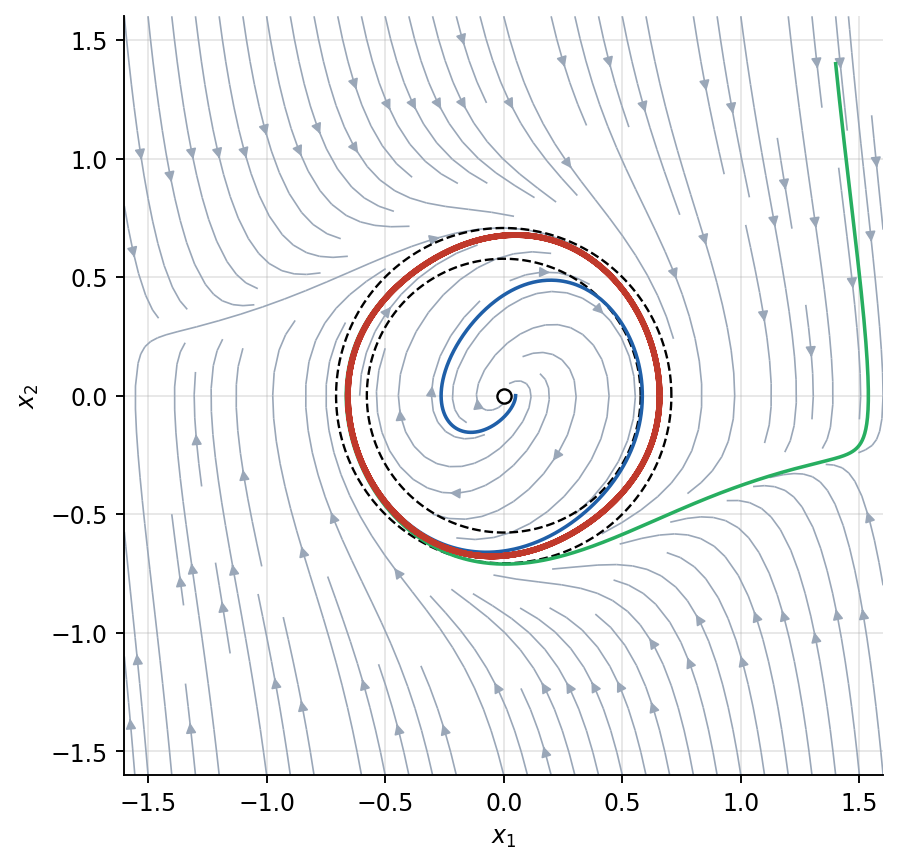
\includegraphics[width=0.6\linewidth,height=\textheight,keepaspectratio,alt={Domaći 1.1: trajektorija iz blizine nule se odmotava, a trajektorija iz (1,4; 1,4) se namotava; obe završe na ciklusu (crveno) koji leži u prstenu između isprekidanih krugova r = √(1/3) i r = √(1/2)}]{figures/nel_dz11.png}
\caption{Domaći 1.1: trajektorija iz blizine nule se odmotava, a trajektorija iz (1,4; 1,4) se namotava; obe završe na ciklusu (crveno) koji leži u prstenu između isprekidanih krugova r = √(1/3) i r = √(1/2)}
\end{figure}

Matlab potvrđuje: na ciklusu je \(r \in [0{,}644;\ 0{,}687]\), unutar prstena \([0{,}577;\ 0{,}707]\).

\subsubsection{Pitanja na odbrani (1.1)}

\begin{enumerate}
\def\labelenumi{\arabic{enumi}.}
\item \textbf{Postoji samo jedna ravnoteža, a sistem ipak trajno osciluje. Kako?} Granični ciklus nije ravnoteža, nego zatvorena trajektorija. Nestabilan fokus gura trajektorije od nule, a za veliko \(r\) član \(x_2(1 - 3x_1^2 - 2x_2^2)\) troši energiju i vraća ih; između toga postoji ciklus.
\item \textbf{Kako znate da je nula nestabilan fokus i da li tu smete da verujete linearizaciji?} \(\tau = 1 > 0\), \(\Delta = 1\), \(\tau^2 < 4\Delta\): kompleksne vrednosti sa pozitivnim realnim delom. Realni deo nije nula (tačka je hiperbolična), pa po Hartman--Grobmanu linearizacija važi lokalno.
\item \textbf{Zašto baš \(V = x_1^2 + x_2^2\)? Da li je to Ljapunovljeva funkcija?} To je kvadrat rastojanja od nule, pa znak \(\dot V\) kaže da li se trajektorija udaljava ili približava. Ovde ne dokazuje stabilnost, nego služi da se konstruiše invarijantan prsten.
\item \textbf{Navedite teoremu koju ste koristili i njene pretpostavke.} Poenkare--Bendikson: zatvoren, ograničen, pozitivno invarijantan skup u \textbf{ravni} koji ne sadrži ravnoteže sadrži periodičnu trajektoriju. Prsten \(1/3 \le r^2 \le 1/2\) ispunjava sve uslove (nula je van njega).
\item \textbf{Da li je ciklus krug?} Nije: u simulaciji \(r\) varira od \(0{,}644\) do \(0{,}687\), jer koeficijenti uz \(x_1^2\) i \(x_2^2\) (3 i 2) nisu jednaki. Teorija garantuje samo da je u prstenu, a Matlab to potvrđuje.
\item \textbf{Kako Matlab potvrđuje zaključak?} Trajektorija iz blizine nule i trajektorija spolja završe na istoj zatvorenoj krivoj, i ta kriva leži između krugova \(r = \sqrt{1/3}\) i \(r = \sqrt{1/2}\).
\item \textbf{Šta bi bilo da je znak zagrade obrnut, \(\dot x_2 = -x_1 - x_2(1 - 3x_1^2 - 2x_2^2)\)?} To je isti sistem u obrnutom vremenu (uz \(x_2 \to -x_2\)): nula postaje stabilan fokus, a ciklus \textbf{nestabilan}, granica oblasti privlačenja nule.
\item \textbf{Zašto linearizacija ne vidi ciklus?} Ona opisuje samo malu okolinu nule; ciklus je na konačnom rastojanju, gde su članovi \(3x_1^2x_2\), \(2x_2^3\) istog reda kao linearni.
\end{enumerate}

\subsection{Domaći 1.2: Khalil 2.4 pod 4}

\[\dot x_1 = -(x_1 - x_1^2) + h(x), \qquad \dot x_2 = -(x_2 - x_2^2) + h(x), \qquad h(x) = 1 - x_1 - x_2\]

Posle uvrštavanja \(h\): \(\dot x_1 = x_1^2 - 2x_1 - x_2 + 1\), \(\dot x_2 = x_2^2 - 2x_2 - x_1 + 1\).

\textbf{Ravnoteže.} Oduzmemo jednačine:

\[(x_1^2 - x_2^2) - (x_1 - x_2) = (x_1 - x_2)(x_1 + x_2 - 1) = 0\]

\begin{itemize}
\item Grana \(x_1 = x_2 = x\): \(x^2 - 3x + 1 = 0\), pa je \(x = (3 \mp \sqrt5)/2\), tj. tačke \((0{,}382;\ 0{,}382)\) i \((2{,}618;\ 2{,}618)\).
\item Grana \(x_2 = 1 - x_1\): \(x_1^2 - 2x_1 - (1 - x_1) + 1 = x_1^2 - x_1 = 0\), tj. tačke \((0, 1)\) i \((1, 0)\).
\end{itemize}

\textbf{Jakobijan i tipovi.}

\[J = \begin{bmatrix} 2x_1 - 2 & -1\\ -1 & 2x_2 - 2\end{bmatrix}\]

\begin{longtable}[]{@{}
  >{\raggedright\arraybackslash}p{(\linewidth - 8\tabcolsep) * \real{0.1739}}
  >{\centering\arraybackslash}p{(\linewidth - 8\tabcolsep) * \real{0.2174}}
  >{\centering\arraybackslash}p{(\linewidth - 8\tabcolsep) * \real{0.2174}}
  >{\centering\arraybackslash}p{(\linewidth - 8\tabcolsep) * \real{0.2174}}
  >{\raggedright\arraybackslash}p{(\linewidth - 8\tabcolsep) * \real{0.1739}}@{}}
\caption{Tačke ravnoteže zadatka 1.2}\tabularnewline
\toprule\noalign{}
\begin{minipage}[b]{\linewidth}\raggedright
Tačka
\end{minipage} & \begin{minipage}[b]{\linewidth}\centering
\(\tau\)
\end{minipage} & \begin{minipage}[b]{\linewidth}\centering
\(\Delta\)
\end{minipage} & \begin{minipage}[b]{\linewidth}\centering
\(\lambda\)
\end{minipage} & \begin{minipage}[b]{\linewidth}\raggedright
Tip
\end{minipage} \\
\midrule\noalign{}
\endfirsthead
\toprule\noalign{}
\begin{minipage}[b]{\linewidth}\raggedright
Tačka
\end{minipage} & \begin{minipage}[b]{\linewidth}\centering
\(\tau\)
\end{minipage} & \begin{minipage}[b]{\linewidth}\centering
\(\Delta\)
\end{minipage} & \begin{minipage}[b]{\linewidth}\centering
\(\lambda\)
\end{minipage} & \begin{minipage}[b]{\linewidth}\raggedright
Tip
\end{minipage} \\
\midrule\noalign{}
\endhead
\bottomrule\noalign{}
\endlastfoot
\((0{,}382;\ 0{,}382)\) & \(-2{,}47\) & \(0{,}53\) & \(-0{,}236;\ -2{,}236\) & stabilan čvor \\
\((2{,}618;\ 2{,}618)\) & \(6{,}47\) & \(9{,}47\) & \(4{,}236;\ 2{,}236\) & nestabilan čvor \\
\((0, 1)\) & \(-2\) & \(-1\) & \(0{,}414;\ -2{,}414\) & sedlo \\
\((1, 0)\) & \(-2\) & \(-1\) & \(0{,}414;\ -2{,}414\) & sedlo \\
\end{longtable}

Za tačke na pravoj \(x_1 = x_2 = a\) matrica je \(\begin{bmatrix}2a - 2 & -1\\ -1 & 2a - 2\end{bmatrix}\), pa su svojstveni vektori \([1, 1]^T\) i \([1, -1]^T\), sa \(\lambda = 2a - 2 \mp 1\). Kod stabilnog čvora (\(a = 0{,}382\)) sporiji pravac je \([1, -1]^T\) (\(\lambda = -0{,}236\)), pa trajektorije ulaze u njega tangentno na pravu \(x_1 + x_2 = \text{const}\). Kod sedla \((0,1)\): \(J = \begin{bmatrix}-2 & -1\ -1 & 0\end{bmatrix}\), \(\lambda^2 + 2\lambda - 1 = 0\), pa je \(\lambda = -1 \pm \sqrt2\). Iz prve vrste \((-2 - \lambda)v_1 = v_2\): nestabilni pravac (\(\lambda = 0{,}414\)) je \([1;\ -2{,}414]^T\), a stabilni (\(\lambda = -2{,}414\)) je \([1;\ 0{,}414]^T\). Za \((1, 0)\) se komponente zamene (simetrija).

\textbf{Ponašanje.} Sistem je simetričan u odnosu na pravu \(x_1 = x_2\) (zamena \(x_1 \leftrightarrow x_2\) ne menja jednačine). Stabilne separatrise sedala polaze iz nestabilnog čvora i omeđuju oblast privlačenja stabilnog čvora. Van nje trajektorije odlaze u beskonačnost (za veliko \(|x|\) dominiraju članovi \(x_1^2\), \(x_2^2\)).

\begin{figure}
\centering
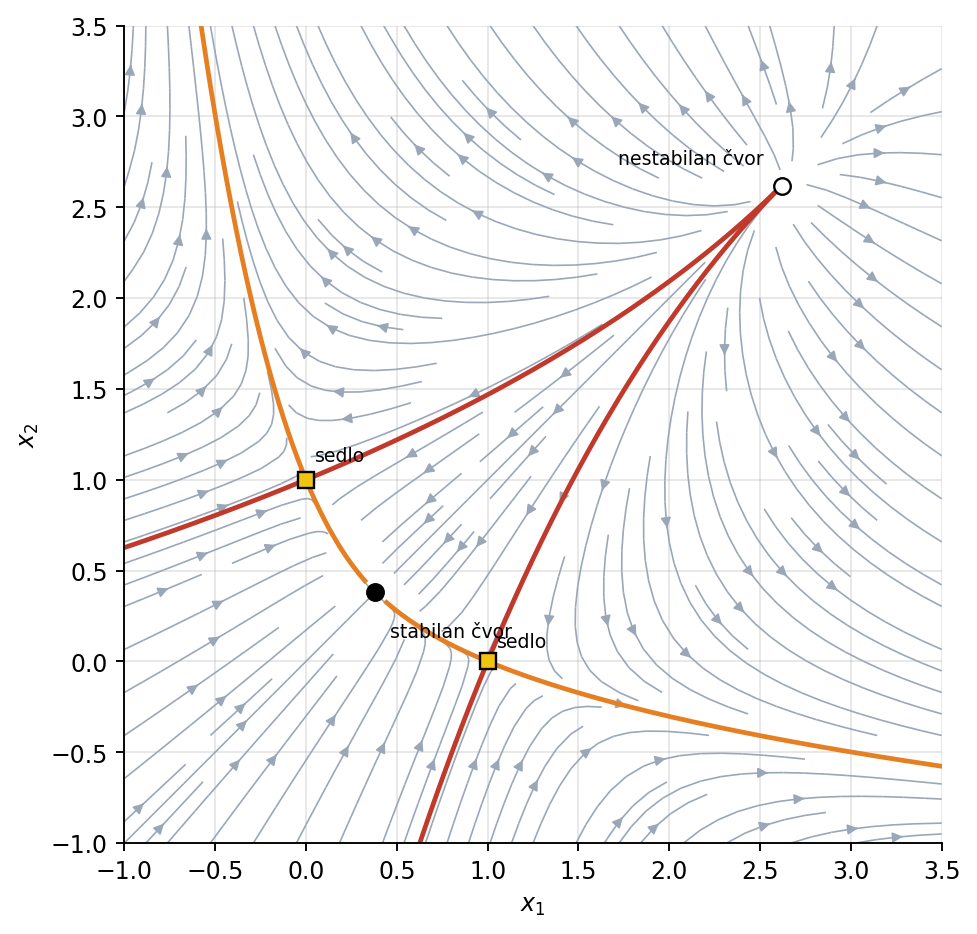
\includegraphics[width=0.65\linewidth,height=\textheight,keepaspectratio,alt={Domaći 1.2: stabilne separatrise sedala (crveno) polaze iz nestabilnog čvora i čine granicu oblasti privlačenja stabilnog čvora; nestabilne separatrise (narandžasto) jednom granom idu u stabilni čvor, a drugom u beskonačnost}]{figures/nel_dz12.png}
\caption{Domaći 1.2: stabilne separatrise sedala (crveno) polaze iz nestabilnog čvora i čine granicu oblasti privlačenja stabilnog čvora; nestabilne separatrise (narandžasto) jednom granom idu u stabilni čvor, a drugom u beskonačnost}
\end{figure}

Poenta zadatka: \textbf{više tačaka ravnoteže}; isti sistem se smiri ili divergira zavisno od početnog stanja.

\subsubsection{Pitanja na odbrani (1.2)}

\begin{enumerate}
\def\labelenumi{\arabic{enumi}.}
\item \textbf{Kako ste našli ravnoteže?} Oduzimanjem jednačina dobija se proizvod \((x_1 - x_2)(x_1 + x_2 - 1) = 0\), pa se rešava po granama; svaka grana daje kvadratnu jednačinu sa dva rešenja.
\item \textbf{Sedlo ima jednu negativnu svojstvenu vrednost. Zašto je ipak nestabilno?} U sedlo ulaze samo trajektorije tačno na stabilnoj separatrisi; svako drugo početno stanje, ma koliko blizu, odlazi duž nestabilnog pravca.
\item \textbf{Šta su separatrise i kako ste ih nacrtali?} Trajektorije koje ulaze u sedlo ili izlaze iz njega duž svojstvenih vektora. Integracija iz tačke malo pomerene od sedla: unazad za stabilne, unapred za nestabilne.
\item \textbf{Šta određuje oblast privlačenja stabilnog čvora?} Stabilne separatrise dva sedla (koje dolaze iz nestabilnog čvora). Unutar njih sve ide u \((0{,}382;\ 0{,}382)\), a van njih u beskonačnost.
\item \textbf{Zašto trajektorije van te oblasti odlaze u beskonačnost?} Za veliko \(|x|\) dominiraju \(x_1^2\) i \(x_2^2\). Na dijagonali je \(\dot x = x^2 - 3x + 1 \approx x^2\), pa iz \(x > 2{,}618\) stanje ode u beskonačnost čak za \textbf{konačno} vreme.
\item \textbf{Po kom pravcu trajektorije ulaze u stabilni čvor?} Tangentno na sporiji svojstveni vektor \([1, -1]^T\) (\(\lambda = -0{,}236\)); brža komponenta duž \([1, 1]^T\) (\(\lambda = -2{,}236\)) nestane ranije.
\item \textbf{Čemu služi simetrija \(x_1 \leftrightarrow x_2\)?} Portret je simetričan u odnosu na pravu \(x_1 = x_2\), pa je dovoljno analizirati jedno sedlo; služi i kao provera Matlab slike.
\item \textbf{Šta je poenta zadatka?} Više izolovanih ravnoteža: isti sistem se smiri ili divergira zavisno od početnog stanja, što linearni sistem ne može.
\end{enumerate}

\subsection{Domaći 1.3: Khalil 2.8}

\[\dot x_1 = x_2, \qquad \dot x_2 = -x_1 + \frac{1}{16}x_1^5 - x_2\]

\begin{enumerate}
\def\labelenumi{(\alph{enumi})}
\item naći ravnoteže i odrediti tip; (b) skicirati portret bez računara (u domaćem i u Matlabu).
\end{enumerate}

\textbf{Ravnoteže.} \(x_2 = 0\) i \(x_1\left(\frac{x_1^4}{16} - 1\right) = 0\), pa je \(x_1 = 0\) ili \(x_1^4 = 16\), tj. \(x_1 = \pm 2\). Tačke su \((0, 0)\), \((2, 0)\) i \((-2, 0)\).

\textbf{Jakobijan.}

\[J = \begin{bmatrix} 0 & 1\\ -1 + \frac{5}{16}x_1^4 & -1\end{bmatrix}\]

\begin{itemize}
\item \((0, 0)\): \(J = \begin{bmatrix}0 & 1\\ -1 & -1\end{bmatrix}\), \(\lambda^2 + \lambda + 1 = 0\), \(\lambda = -0{,}5 \pm j0{,}866\): \textbf{stabilan fokus}.
\item \((\pm 2, 0)\): \(-1 + \frac{5}{16}\cdot 16 = 4\), pa je \(J = \begin{bmatrix}0 & 1\\ 4 & -1\end{bmatrix}\), \(\lambda^2 + \lambda - 4 = 0\), \(\lambda = \frac{-1 \pm \sqrt{17}}{2} = 1{,}56\) i \(-2{,}56\): \textbf{sedla}.
\end{itemize}

Za matricu oblika \(\begin{bmatrix}0 & 1\\ a & b\end{bmatrix}\) svojstveni vektor za \(\lambda\) je \([1, \lambda]^T\) (iz prve vrste: \(v_2 = \lambda v_1\)). Zato je nestabilni pravac sedla \([1;\ 1{,}56]^T\), a stabilni \([1;\ -2{,}56]^T\).

\textbf{Skica bez računara}, korak po korak:

\begin{enumerate}
\def\labelenumi{\arabic{enumi}.}
\item Oko nule trajektorije se spiralno uvijaju ka \((0,0)\), u smeru kazaljke na satu (\(\dot x_1 = x_2 > 0\) gore).
\item Kroz svako sedlo nacrtati dve prave: stabilni pravac (strmo opadajući, nagib \(-2{,}56\)) sa strelicama ka sedlu i nestabilni (nagib \(1{,}56\)) sa strelicama od sedla.
\item Stabilne separatrise sedala zatvaraju „traku'' oko nule: to je \textbf{oblast privlačenja} fokusa.
\item Unutrašnje nestabilne separatrise sedala završavaju u fokusu, a spoljašnje idu u beskonačnost (za veliko \(|x_1|\) dominira \(x_1^5/16\), koji gura dalje od nule).
\item Periodičnih trajektorija nema: \(\operatorname{div} f = 0 + (-1) = -1 < 0\) svuda, pa po Bendiksonovom kriterijumu ciklusa nema. Skica je zato potpuna.
\end{enumerate}

\begin{figure}
\centering
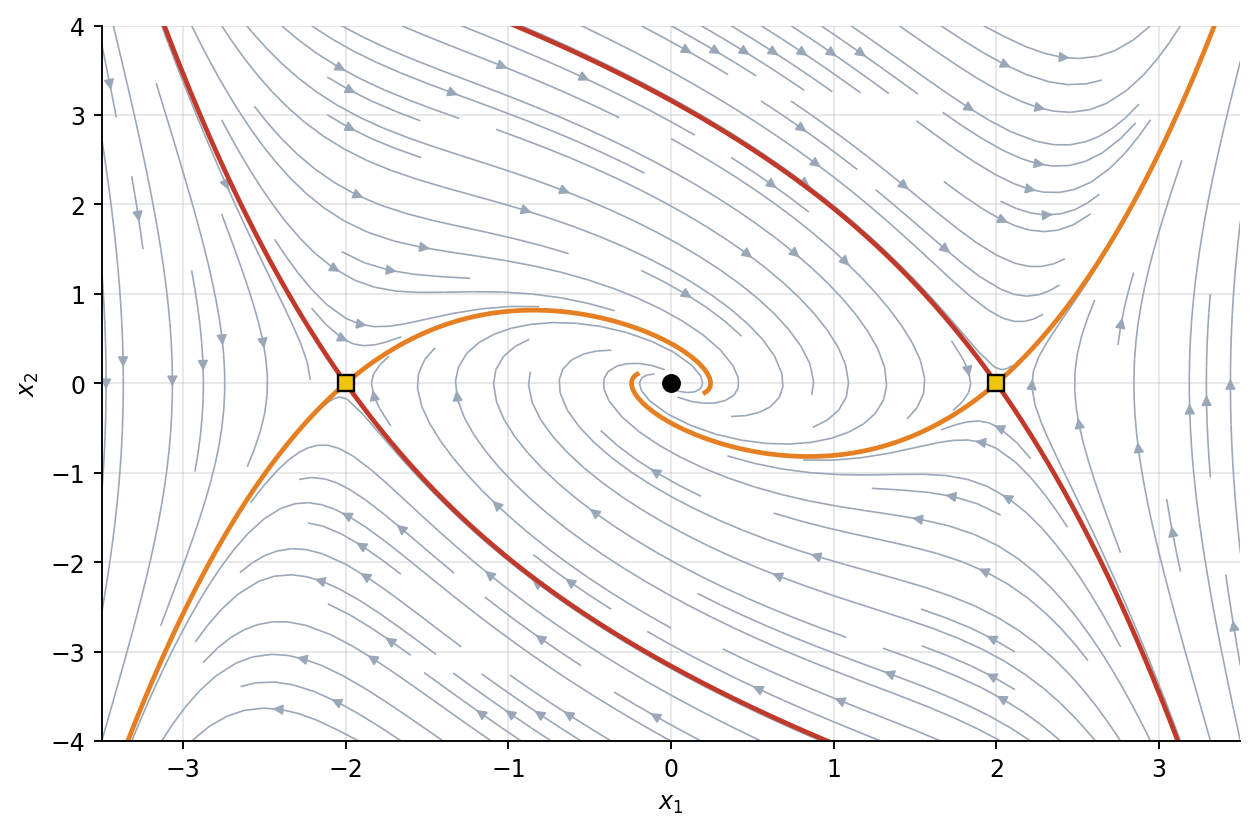
\includegraphics[width=0.75\linewidth,height=\textheight,keepaspectratio,alt={Domaći 1.3: stabilne separatrise sedala (±2, 0) (crveno) omeđuju oblast privlačenja stabilnog fokusa u nuli; unutrašnje nestabilne separatrise (narandžasto) se uvijaju u nulu, a spoljašnje odlaze u beskonačnost}]{figures/nel_dz13.png}
\caption{Domaći 1.3: stabilne separatrise sedala (±2, 0) (crveno) omeđuju oblast privlačenja stabilnog fokusa u nuli; unutrašnje nestabilne separatrise (narandžasto) se uvijaju u nulu, a spoljašnje odlaze u beskonačnost}
\end{figure}

Linearizacija bi dala samo „stabilan fokus''. Tek portret pokazuje da je stabilnost \textbf{lokalna}: iz početnog stanja van trake sistem divergira. Bendiksonov argument je dodat ovde (nema ga u referentnom rešenju).

\subsubsection{Pitanja na odbrani (1.3)}

\begin{enumerate}
\def\labelenumi{\arabic{enumi}.}
\item \textbf{Kako ste skicirali portret bez računara?} Ravnoteže i njihov tip, pravci svojstvenih vektora sedala, smer obrtanja oko fokusa i ponašanje za veliko \(|x_1|\); Bendikson isključuje cikluse, pa ništa drugo ne može postojati.
\item \textbf{Zašto su \((\pm2, 0)\) sedla, bez računanja korena?} \(\Delta = \det J = -4 < 0\), pa su svojstvene vrednosti realne i suprotnog znaka.
\item \textbf{Zašto je svojstveni vektor \([1, \lambda]^T\)?} Prva vrsta Jakobijana je \([0\ \ 1]\), pa iz \(Jv = \lambda v\) sledi \(v_2 = \lambda v_1\).
\item \textbf{Iskažite Bendiksonov kriterijum i zašto važi.} Ako \(\operatorname{div} f\) ne menja znak (i nije identički nula) u jednostruko povezanoj oblasti, nema zatvorenih trajektorija. Duž zatvorene trajektorije je \(\oint(f_1dx_2 - f_2dx_1) = 0\), a po Grinovoj teoremi to je \(\iint\operatorname{div} f\,dA\), što bi ovde bilo \(-\)površina \(\ne 0\).
\item \textbf{Da li je nula globalno stabilna?} Nije, samo lokalno: oblast privlačenja je traka između stabilnih separatrisa sedala; van nje rešenje divergira.
\item \textbf{Kakav je ovo fizički sistem?} Masa sa trenjem (\(-x_2\)) i „mekom'' oprugom \(-x_1 + x_1^5/16\): za \(|x_1| > 2\) opruga više ne vraća, nego gura dalje.
\item \textbf{Šta bi bilo bez trenja (bez \(-x_2\))?} Linearizacija u nuli daje centar, a sistem je konzervativan (\(E = \frac12x_2^2 + \frac12x_1^2 - \frac{x_1^6}{96}\) je konstantno), pa je nula pravi centar okružen zatvorenim orbitama unutar separatrisa; \(\operatorname{div} f = 0\), pa Bendikson ne važi.
\item \textbf{Kako Matlab potvrđuje?} Trajektorije iz trake se spiralno uvijaju u nulu, a one izvan nje odlaze u beskonačnost; separatrise dobijene integracijom su granica.
\end{enumerate}

\begin{ispit}
Za svaki portret umeti usmeno: (1) kako su nađene ravnoteže, (2) Jakobijan i tip po svojstvenim vrednostima, (3) šta su separatrise i kako su nacrtane u Matlabu, (4) šta linearizacija \textbf{ne vidi} (granični ciklus u 1.1, oblast privlačenja u 1.2 i 1.3). Zamka: za centar linearizacija ne daje zaključak. Druga zamka: stabilan fokus u nuli ne znači globalnu stabilnost.
\end{ispit}

\section{Ljapunovljeva stabilnost}

\subsection{Ideja}

Kod linearnih sistema stabilnost se čita iz polova. Kod nelinearnih polova nema, a linearizacija važi samo lokalno i ne radi kada je \(\operatorname{Re}\lambda = 0\). Ljapunov nudi drugi put: nađe se funkcija \(V(x)\) koja se ponaša kao \textbf{energija} (nula u ravnoteži, pozitivna svuda drugde) i pokaže se da duž trajektorija \textbf{ne raste}. Tada sistem ne može da pobegne od ravnoteže. Ova teorija je rađena u adaptivnom delu predmeta (tamo za dokaze konvergencije zakona adaptacije); ovde je pun pregled onoga što se koristi u nelinearnom delu.

\subsection{Definicije stabilnosti}

Posmatramo \(\dot x = f(x)\) sa ravnotežom \(x_0\).

\begin{itemize}
\item \textbf{Stabilnost (po Ljapunovu)}: za svako \(\varepsilon > 0\) postoji \(\delta > 0\) tako da
  \[\|x(0) - x_0\| < \delta \;\Rightarrow\; \|x(t) - x_0\| < \varepsilon \quad \forall t \ge 0\]
  Ako se krene dovoljno blizu, trajektorija \textbf{ostaje} blizu. Ne mora da stigne u \(x_0\).
\item \textbf{Asimptotska stabilnost}: stabilnost i još \(\lim_{t\to\infty} x(t) = x_0\).
\item \textbf{Eksponencijalna stabilnost}: postoje \(M, \lambda > 0\) tako da je \(\|x(t) - x_0\| \le M\|x(0) - x_0\|e^{-\lambda t}\) za svako \(t \ge 0\).
\end{itemize}

Važi: eksponencijalna \(\Rightarrow\) asimptotska \(\Rightarrow\) stabilnost. Stabilnost linearnog sistema sa polovima u levoj poluravni je uvek eksponencijalna.

Ako asimptotska stabilnost važi za \textbf{svako} početno stanje, ravnoteža je \textbf{globalno asimptotski stabilna} (GAS).

\subsection{Pozitivno definitna funkcija}

\(V: \mathbb{R}^n \to \mathbb{R}\) je \textbf{pozitivno definitna} u oblasti \(B\) oko nule ako je \(V(0) = 0\) i \(V(x) > 0\) za svako \(x \in B\), \(x \ne 0\). Ako je samo \(V(x) \ge 0\), funkcija je pozitivno \textbf{semidefinitna}. Tipičan primer: \(V = \frac12(x_1^2 + x_2^2)\).

\subsection{Teorema Ljapunova (direktna metoda)}

Neka je \(V\) neprekidno diferencijabilna i pozitivno definitna oko ravnoteže \(x_0\) (za \(x_0 \ne 0\) se \(V\) piše po odstupanju \(x - x_0\)), i neka je njen izvod duž trajektorija (pravilo lanca: \(\frac{d}{dt}V(x(t)) = \sum_i \frac{\partial V}{\partial x_i}\dot x_i\))

\[\dot V(x) = \frac{\partial V}{\partial x}\dot x = \frac{\partial V}{\partial x}f(x)\]

Tada:

\begin{itemize}
\item \(\dot V \le 0\): ravnoteža je \textbf{stabilna};
\item \(\dot V < 0\) za \(x \ne x_0\): ravnoteža je \textbf{asimptotski stabilna}.
\end{itemize}

Za \textbf{globalnu} asimptotsku stabilnost treba još da \(V\) bude \textbf{radijalno neograničena}: \(V(x) \to \infty\) kada \(\|x\| \to \infty\) \izvor{standardna teorija, Khalil teorema 4.2}. Bez toga nivo-krive \(V = c\) za veliko \(c\) ne moraju biti zatvorene, pa trajektorija može otići u beskonačnost iako \(V\) opada.

\textbf{Nestabilnost (Četajev)} \izvor{standardna teorija, Khalil teorema 4.3}: ako postoji \(V\) sa \(V(0) = 0\), koja je pozitivna u tačkama proizvoljno blizu nule, i za koju je \(\dot V > 0\) u okolini nule (osim u nuli), ravnoteža je \textbf{nestabilna}. Ovo je jedini ispravan način da se „iz \(V\)„ zaključi nestabilnost; tako je urađeno u domaćem 3.2 (sistem 1).

\begin{kljucna}
Uslov je \textbf{dovoljan, ne i potreban}. Ako za izabrano \(V\) ne dobijemo \(\dot V \le 0\), to ne znači da je sistem nestabilan; možda samo nismo našli dobru funkciju.
\end{kljucna}

\textbf{Kako izabrati \(V\)}: nema pravila. U \(V\) se stavlja ono što želimo da iščezne (stanja, greške), najčešće kvadratno: \(V = \frac12\sum x_i^2\). Zatim se \(V\) prilagodi tako da se u \(\dot V\) skrate „loši'' članovi. Upravo to radi backstepping: \(V\) se gradi korak po korak, a upravljanje se bira tako da \(\dot V\) bude negativno.

\subsubsection{Primer sa predavanja}

\[\dot x_1 = -x_1^3 + 2x_2^3, \qquad \dot x_2 = -2x_1x_2^2\]

Kandidat \(V = \frac12(x_1^2 + x_2^2)\):

\[\dot V = x_1(-x_1^3 + 2x_2^3) + x_2(-2x_1x_2^2) = -x_1^4 + 2x_1x_2^3 - 2x_1x_2^3 = -x_1^4 \le 0\]

Nula je \textbf{stabilna}. Ovaj \(V\) ne daje asimptotsku stabilnost, jer je \(\dot V = 0\) na celoj osi \(x_1 = 0\).

\subsubsection{Kada je izvod samo semidefinitan: LaSalle}

Ako je \(\dot V \le 0\), trajektorije završavaju u najvećem invarijantnom skupu unutar skupa \(\{x : \dot V(x) = 0\}\) \izvor{standardna teorija, Khalil teorema 4.4}. Ako taj skup sadrži samo ravnotežu, ona je asimptotski stabilna. U primeru iznad: na osi \(x_1 = 0\) je \(\dot x_1 = 2x_2^3 \ne 0\) za \(x_2 \ne 0\), pa trajektorija ne ostaje na osi; jedini invarijantan deo ose je nula. Dakle nula je u stvari asimptotski stabilna, i to globalno, jer je \(V\) radijalno neograničena (pa su sve trajektorije ograničene, što LaSalle traži).

\subsection{Veza sa linearizacijom (indirektna metoda)}

Isto pravilo kao kod faznih portreta (Hartman--Grobman, poglavlje „Fazna ravan''): sve svojstvene vrednosti Jakobijana levo daje lokalno eksponencijalnu stabilnost, neka desno nestabilnost, a neka na imaginarnoj osi ne daje zaključak \izvor{standardna teorija, Khalil teorema 4.7}. Tada se koristi Ljapunov (npr. domaći 3.3).

\subsection{Gde se koristi u domaćim zadacima}

\begin{longtable}[]{@{}
  >{\raggedright\arraybackslash}p{(\linewidth - 4\tabcolsep) * \real{0.1683}}
  >{\raggedright\arraybackslash}p{(\linewidth - 4\tabcolsep) * \real{0.3465}}
  >{\raggedright\arraybackslash}p{(\linewidth - 4\tabcolsep) * \real{0.4851}}@{}}
\caption{Ljapunovljeve funkcije u domaćim zadacima}\tabularnewline
\toprule\noalign{}
\begin{minipage}[b]{\linewidth}\raggedright
Zadatak
\end{minipage} & \begin{minipage}[b]{\linewidth}\raggedright
Funkcija \(V\)
\end{minipage} & \begin{minipage}[b]{\linewidth}\raggedright
Zaključak
\end{minipage} \\
\midrule\noalign{}
\endfirsthead
\toprule\noalign{}
\begin{minipage}[b]{\linewidth}\raggedright
Zadatak
\end{minipage} & \begin{minipage}[b]{\linewidth}\raggedright
Funkcija \(V\)
\end{minipage} & \begin{minipage}[b]{\linewidth}\raggedright
Zaključak
\end{minipage} \\
\midrule\noalign{}
\endhead
\bottomrule\noalign{}
\endlastfoot
1.1 & \(V = x_1^2 + x_2^2\) & prsten u kome postoji granični ciklus \\
3.2, sistem 1 & \(V = \frac12x_1^2\) & \(\dot V > 0\) (Četajev): nulta dinamika \(\dot x_1 = \operatorname{tg}x_1\) nestabilna \\
3.2, sistem 2 & \(V = \frac12(x_1^2 + x_2^2)\) & \(\dot V = -(x_1 - x_2)^2 \le 0\): stabilna, ne asimptotski \\
3.3 & \(V = \frac12\eta^2\) & \(\dot V = -\eta^4 < 0\): GAS, minimalna faza \\
4.2 & \(V = \frac12x_1^2 + \frac12z_2^2\) & \(\dot V < 0\): GAS zatvorene sprege \\
\end{longtable}

\begin{ispit}
Razlikovati stabilnost i asimptotsku stabilnost (\(\le\) naspram \(<\)). Kod zaključka „GAS'' uvek reći da je \(V\) radijalno neograničena. Nikad ne zaključivati nestabilnost iz toga što \(\dot V\) nije negativno; nestabilnost traži \(\dot V > 0\) (Četajev) ili linearizaciju sa \(\operatorname{Re}\lambda > 0\).
\end{ispit}

\section{Opisna funkcija i harmonijski balans}

\subsection{Ideja}

Linearni sistem na sinusni ulaz odgovara sinusom iste frekvencije, pa se opisuje funkcijom prenosa \(G(j\omega)\). Nelinearnost na sinusni ulaz daje izlaz sa višim harmonicima. Ako je linearni deo petlje niskopropusni filtar, viši harmonici se priguše, i ostaje samo prvi. Zato nelinearnost zamenjujemo „pojačanjem za prvi harmonik'' \(N(A)\), koje zavisi od amplitude ulaza. Sa tom zamenom se pitanje „da li sistem osciluje'' svodi na presek dve krive u kompleksnoj ravni: \(G(j\omega)\) i \(-1/N(A)\).

\subsection{Klasa sistema i pretpostavke}

Analiziramo petlju: referenca \(r = 0\), greška \(e\) ulazi u statičku nelinearnost \(f\), njen izlaz \(v\) ulazi u linearni deo \(G(s)\), a izlaz \(y\) se vraća sa negativnim znakom, \(e = -y\).

Pretpostavke:

\begin{enumerate}
\def\labelenumi{\arabic{enumi}.}
\item \(r = 0\), pa je \(e = -y\).
\item \(G(s)\) je \textbf{niskopropusni filtar}: propušta prvi harmonik, a više guši.
\item Nelinearnost je \textbf{statička} (ne zavisi od frekvencije ulaza, samo od vrednosti i eventualno smera promene, kao kod histerezisa).
\end{enumerate}

Mehanizam: \(e = A\sin\omega t\); \(v\) sadrži sve harmonike; \(G\) ih isfiltrira; \(y\) je (približno) sinusoida; \(e = -y\) je opet sinusoida, pa se petlja zatvara.

\subsection{Definicija opisne funkcije}

Za ulaz \(e = A\sin\theta\), \(\theta = \omega t\), izlaz nelinearnosti razvijemo u Furijeov red:

\[v = f(A\sin\theta) = b_0 + a_1\sin\theta + b_1\cos\theta + \text{viši harmonici}\]

\[b_0 = \frac{1}{2\pi}\int_0^{2\pi} f(A\sin\theta)\,d\theta, \qquad a_1 = \frac{1}{\pi}\int_0^{2\pi} f(A\sin\theta)\sin\theta\,d\theta, \qquad b_1 = \frac{1}{\pi}\int_0^{2\pi} f(A\sin\theta)\cos\theta\,d\theta\]

Sa \(a_1 = R\cos\varphi\) i \(b_1 = R\sin\varphi\) prvi harmonik je \(R\sin(\theta + \varphi)\), jer je \(R\sin(\theta + \varphi) = R\cos\varphi\sin\theta + R\sin\varphi\cos\theta\). \textbf{Opisna funkcija} je odnos prvog harmonika izlaza i ulaza, u kompleksnom obliku:

\[N(A) = \frac{a_1 + jb_1}{A} = \frac{\sqrt{a_1^2 + b_1^2}}{A}\,e^{j\varphi}, \qquad \varphi = \operatorname{arctg}\frac{b_1}{a_1}\]

\(N\) zavisi od amplitude \(A\), a ne od \(\omega\) (pretpostavka 3).

Dve simetrije skraćuju račun:

\begin{itemize}
\item \textbf{Neparna} nelinearnost, \(f(-e) = -f(e)\): izlaz nema srednju vrednost, \(b_0 = 0\).
\item \textbf{Jednoznačna} neparna nelinearnost (bez histerezisa): \(f(A\sin\theta)\) je neparna funkcija od \(\theta\), pa su svi kosinusni koeficijenti nula, \(b_1 = 0\). Tada je \(N(A)\) \textbf{realna} (bez faznog pomaka). Pored toga je izlaz simetričan oko \(\theta = \pi/2\), pa je \(a_1 = \frac{4}{\pi}\int_0^{\pi/2} f(A\sin\theta)\sin\theta\,d\theta\).
\end{itemize}

Histerezis nije jednoznačan (izlaz zavisi od smera), pa kod njega \(b_1 \ne 0\) i \(N(A)\) je kompleksna. Znak konvencije: \(b_1 < 0\) znači da prvi harmonik izlaza \textbf{kasni} za ulazom.

\subsection{Opisne funkcije tipičnih nelinearnosti}

\subsubsection{Idealni relej ±K}

Izlaz je četvrtka: \(+K\) na \((0, \pi)\), \(-K\) na \((\pi, 2\pi)\). Jednoznačna i neparna, pa je \(b_0 = b_1 = 0\) i

\[a_1 = \frac{4}{\pi}\int_0^{\pi/2} K\sin\theta\,d\theta = \frac{4K}{\pi}\big[-\cos\theta\big]_0^{\pi/2} = \frac{4K}{\pi}, \qquad N(A) = \frac{4K}{\pi A}\]

Relej uvek daje isti izlaz, pa je relativno pojačanje manje što je ulaz veći.

\subsubsection{Relej sa mrtvom zonom}

Izlaz \(\pm K\), mrtva zona \(|e| < \varepsilon\). Za \(A > \varepsilon\) relej uključuje na uglu \(\beta\), gde je \(A\sin\beta = \varepsilon\):

\[a_1 = \frac{4}{\pi}\int_\beta^{\pi/2} K\sin\theta\,d\theta = \frac{4K}{\pi}\cos\beta, \qquad N(A) = \frac{4K}{\pi A}\sqrt{1 - \frac{\varepsilon^2}{A^2}}, \quad A > \varepsilon\]

Za \(A \le \varepsilon\) je \(N = 0\). \(N(A)\) nije monotona: \(N \propto \sqrt{A^2 - \varepsilon^2}/A^2\), a izvod ovog izraza je nula za \(A^2 = 2\varepsilon^2\), pa je maksimum \(\frac{2K}{\pi\varepsilon}\) za \(A = \varepsilon\sqrt2\), pa \(-1/N(A)\) ide od \(-\infty\) do \(-\frac{\pi\varepsilon}{2K}\) i nazad. Zato mogu postojati dva preseka sa Nikvistovom krivom: jedan nestabilan i jedan stabilan ciklus.

\subsubsection{Domaći 2.1 a): zasićenje}

Zasićenje sa nagibom \(k\) i pragom \(\varepsilon\): \(f(e) = ke\) za \(|e| \le \varepsilon\), a \(f(e) = k\varepsilon\operatorname{sign}(e)\) za \(|e| > \varepsilon\).

\textbf{Slučaj \(A \le \varepsilon\)}: element radi linearno, \(v = kA\sin\theta\), pa je \(N(A) = k\).

\textbf{Slučaj \(A > \varepsilon\)}: izlaz prati \(kA\sin\theta\) do ugla \(\beta\) u kome ulaz dostigne prag,

\[A\sin\beta = \varepsilon \quad\Rightarrow\quad \beta = \arcsin\frac{\varepsilon}{A}\]

a zatim je konstantan \(k\varepsilon\) do \(\pi - \beta\). Nelinearnost je jednoznačna i neparna, pa je \(b_0 = b_1 = 0\), a \(a_1\) se računa na četvrtini periode:

\[a_1 = \frac{4}{\pi}\left[\int_0^\beta kA\sin^2\theta\,d\theta + \int_\beta^{\pi/2} k\varepsilon\sin\theta\,d\theta\right]\]

Prvi integral, uz \(\sin^2\theta = \frac{1 - \cos2\theta}{2}\):

\[\int_0^\beta kA\sin^2\theta\,d\theta = kA\left[\frac{\theta}{2} - \frac{\sin2\theta}{4}\right]_0^\beta = kA\left(\frac{\beta}{2} - \frac{\sin2\beta}{4}\right)\]

Drugi integral:

\[\int_\beta^{\pi/2} k\varepsilon\sin\theta\,d\theta = k\varepsilon\big[-\cos\theta\big]_\beta^{\pi/2} = k\varepsilon\cos\beta\]

Pošto je \(\varepsilon = A\sin\beta\), važi \(kA\frac{\sin2\beta}{4} = kA\frac{\sin\beta\cos\beta}{2} = \frac{k\varepsilon\cos\beta}{2}\). Zato

\[a_1 = \frac{4k}{\pi}\left[\frac{A\beta}{2} - \frac{\varepsilon\cos\beta}{2} + \varepsilon\cos\beta\right] = \frac{2kA}{\pi}\left[\beta + \frac{\varepsilon}{A}\cos\beta\right]\]

Deljenjem sa \(A\) i uz \(\cos\beta = \sqrt{1 - \varepsilon^2/A^2}\):

\begin{kljucna}
\[N_{zas}(A) = \frac{2k}{\pi}\left[\arcsin\frac{\varepsilon}{A} + \frac{\varepsilon}{A}\sqrt{1 - \frac{\varepsilon^2}{A^2}}\right], \quad A > \varepsilon; \qquad N_{zas}(A) = k, \quad A \le \varepsilon\]
\end{kljucna}

Provere:

\begin{itemize}
\item za \(A \to \varepsilon\) je \(\beta = \pi/2\), pa je \(N = \frac{2k}{\pi}\cdot\frac{\pi}{2} = k\): nastavlja se neprekidno na linearni deo;
\item za \(A \to \infty\) je \(\arcsin x \approx x\), pa je \(N \approx \frac{4k\varepsilon}{\pi A}\): to je relej sa izlazom \(\pm k\varepsilon\), kako i treba;
\item \(N\) je realna i opada od \(k\) ka nuli, pa \(-1/N(A)\) ide po negativnoj realnoj osi od \(-1/k\) ka \(-\infty\).
\end{itemize}

Ako se zasićenje parametrizuje \textbf{nivoom} \(K\) (nagib \(K/\varepsilon\)), dobija se \(N = \frac{2K}{\pi\varepsilon}\left[\arcsin\frac{\varepsilon}{A} + \frac{\varepsilon}{A}\sqrt{1 - \frac{\varepsilon^2}{A^2}}\right]\); sa \(K = k\varepsilon\) to je isti izraz.

\subsubsection{Domaći 2.1 b): relej sa histerezisom}

Izlaz \(\pm K\), histerezis širine \(2\delta\): prebacuje se na \(+K\) kada ulaz \textbf{raste} preko \(+\delta\), a na \(-K\) kada \textbf{opada} ispod \(-\delta\).

Za \(e = A\sin\theta\), \(A > \delta\): u prethodnoj periodi ulaz je na \(\theta = \pi + \alpha\) pao ispod \(-\delta\) i od tada nije prešao \(+\delta\), pa je u \(\theta = 0\) izlaz \(-K\) (iako je sam ulaz tada nula). Ulaz raste i prelazi \(+\delta\) na uglu

\[\alpha = \arcsin\frac{\delta}{A}\]

kada izlaz skače na \(+K\). Ulaz zatim opada i prelazi \(-\delta\) na \(\theta = \pi + \alpha\) (jer je \(A\sin(\pi + \alpha) = -\delta\)). Dakle izlaz je \textbf{četvrtka zakašnjela za \(\alpha\)}: \(-K\) na \([0, \alpha)\), \(+K\) na \([\alpha, \pi + \alpha)\), \(-K\) na \([\pi + \alpha, 2\pi)\).

Koeficijent \(a_1\):

\[a_1 = \frac{K}{\pi}\left[\int_\alpha^{\pi + \alpha}\sin\theta\,d\theta - \int_0^\alpha\sin\theta\,d\theta - \int_{\pi + \alpha}^{2\pi}\sin\theta\,d\theta\right]\]

Tri integrala: \(\int_\alpha^{\pi+\alpha}\sin\theta\,d\theta = \cos\alpha - \cos(\pi + \alpha) = 2\cos\alpha\); \(\int_0^\alpha\sin\theta\,d\theta = 1 - \cos\alpha\); \(\int_{\pi+\alpha}^{2\pi}\sin\theta\,d\theta = -1 + \cos(\pi + \alpha) = -1 - \cos\alpha\). Zato

\[a_1 = \frac{K}{\pi}\left[2\cos\alpha - (1 - \cos\alpha) + (1 + \cos\alpha)\right] = \frac{4K}{\pi}\cos\alpha\]

Koeficijent \(b_1\), istim postupkom sa \(\cos\theta\): \(\int_\alpha^{\pi+\alpha}\cos\theta\,d\theta = \sin(\pi + \alpha) - \sin\alpha = -2\sin\alpha\); \(\int_0^\alpha\cos\theta\,d\theta = \sin\alpha\); \(\int_{\pi+\alpha}^{2\pi}\cos\theta\,d\theta = 0 - \sin(\pi + \alpha) = \sin\alpha\). Zato

\[b_1 = \frac{K}{\pi}\left[-2\sin\alpha - \sin\alpha - \sin\alpha\right] = -\frac{4K}{\pi}\sin\alpha\]

\begin{kljucna}
\[N_{hist}(A) = \frac{4K}{\pi A}\left(\cos\alpha - j\sin\alpha\right) = \frac{4K}{\pi A}e^{-j\alpha} = \frac{4K}{\pi A}\left[\sqrt{1 - \frac{\delta^2}{A^2}} - j\frac{\delta}{A}\right], \qquad \alpha = \arcsin\frac{\delta}{A}\]
\end{kljucna}

Moduo je isti kao kod idealnog releja, \(|N| = \frac{4K}{\pi A}\) (isto sledi iz \(a_1^2 + b_1^2 = \frac{16K^2}{\pi^2}\)), a argument je \(-\alpha\): histerezis unosi \textbf{kašnjenje}, jer relej prebacuje tek kada ulaz pređe prag. Faza se može pisati i kao \(-\operatorname{arctg}\frac{\delta}{\sqrt{A^2 - \delta^2}}\), što je isti ugao.

Kritična kriva:

\[-\frac{1}{N(A)} = -\frac{\pi A}{4K}e^{j\alpha} = -\frac{\pi}{4K}\left(A\cos\alpha + jA\sin\alpha\right) = -\frac{\pi}{4K}\left(\sqrt{A^2 - \delta^2} + j\delta\right)\]

To je \textbf{horizontalna prava} \(\operatorname{Im} = -\frac{\pi\delta}{4K}\), koja sa rastom \(A\) ide od \(\operatorname{Re} = 0\) ka \(-\infty\). Za \(\delta = 0\) dobija se idealni relej.

\begin{figure}
\centering
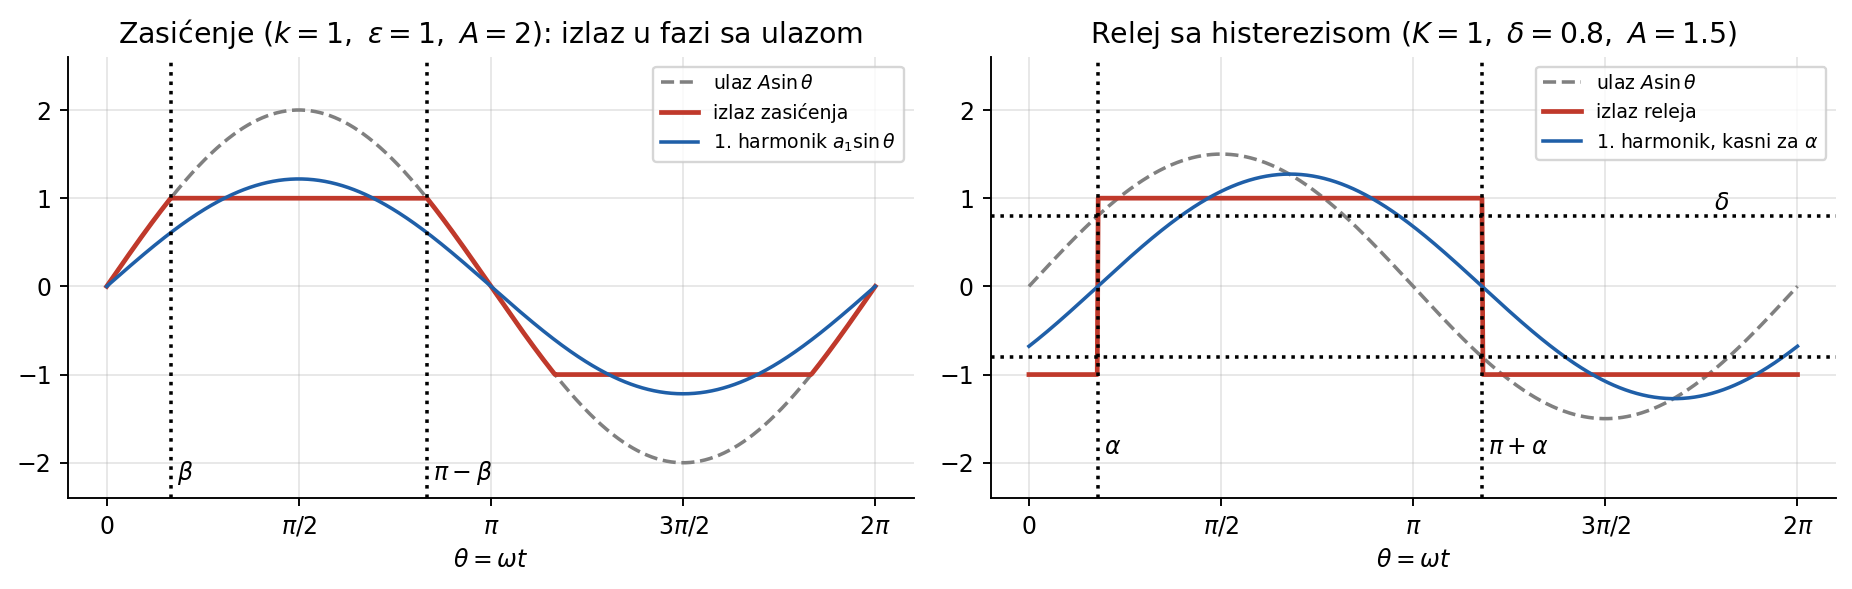
\includegraphics[width=0.95\linewidth,height=\textheight,keepaspectratio,alt={Levo: zasićenje odseca vrh sinusoide, a prvi harmonik izlaza je u fazi sa ulazom. Desno: relej sa histerezisom daje četvrtku zakašnjelu za α, pa i njen prvi harmonik kasni za α}]{figures/nel_df_talasi.png}
\caption{Levo: zasićenje odseca vrh sinusoide, a prvi harmonik izlaza je u fazi sa ulazom. Desno: relej sa histerezisom daje četvrtku zakašnjelu za α, pa i njen prvi harmonik kasni za α}
\end{figure}

\begin{figure}
\centering
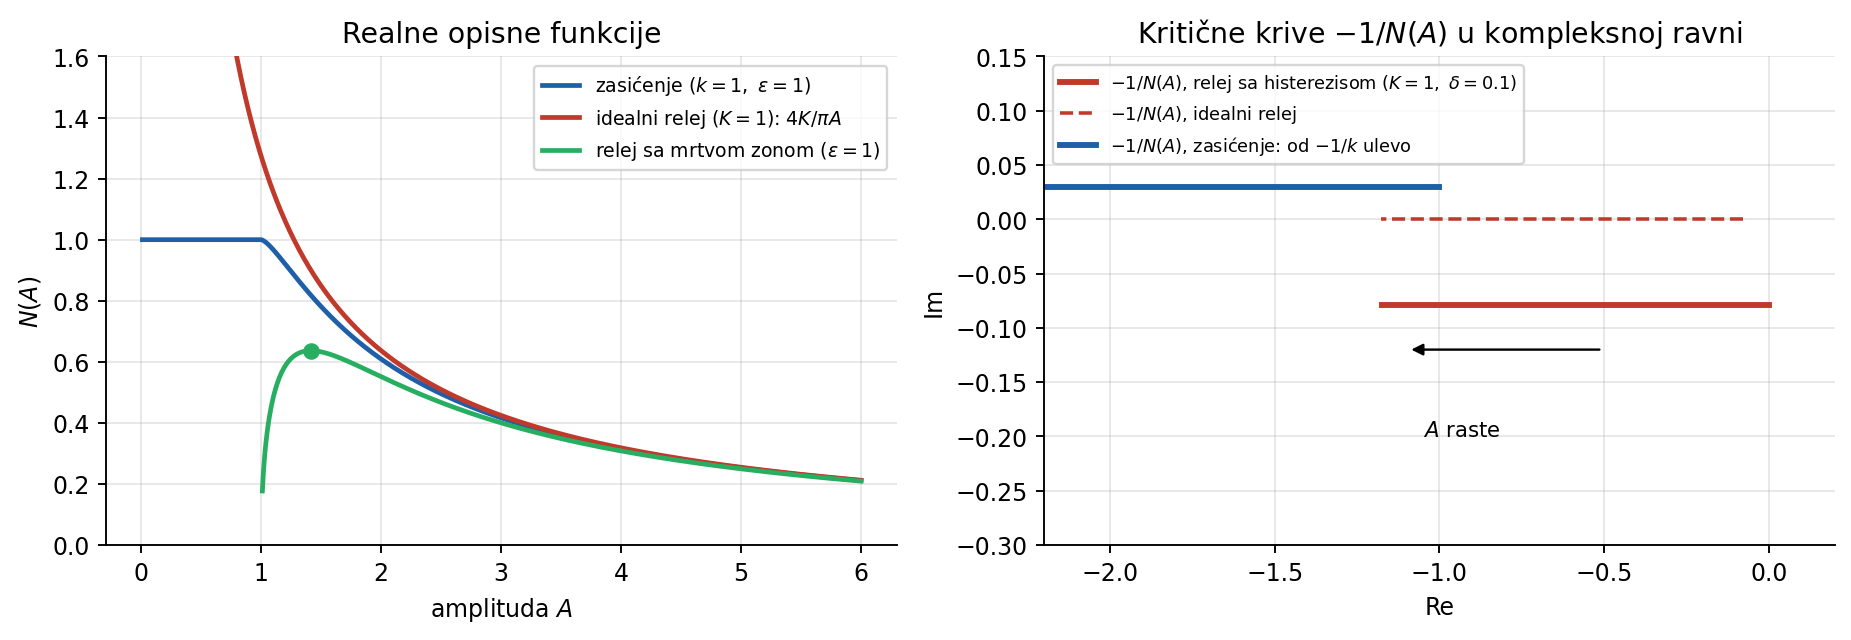
\includegraphics[width=0.95\linewidth,height=\textheight,keepaspectratio,alt={Levo: realne opisne funkcije (zasićenje počinje od k i opada; relej sa mrtvom zonom ima maksimum). Desno: kritične krive -1/N(A); zasićenje i idealni relej leže na negativnoj realnoj osi, a relej sa histerezisom na horizontalnoj pravi ispod nje}]{figures/nel_df_N.png}
\caption{Levo: realne opisne funkcije (zasićenje počinje od k i opada; relej sa mrtvom zonom ima maksimum). Desno: kritične krive -1/N(A); zasićenje i idealni relej leže na negativnoj realnoj osi, a relej sa histerezisom na horizontalnoj pravi ispod nje}
\end{figure}

\subsubsection{Pitanja na odbrani (2.1)}

\begin{enumerate}
\def\labelenumi{\arabic{enumi}.}
\item \textbf{Zašto se zadržava samo prvi harmonik?} Pretpostavka je da linearni deo petlje \(G(s)\) niskopropusno guši više harmonike, pa se u povratnoj sprezi vraća praktično samo prvi.
\item \textbf{Zašto je kod zasićenja \(b_0 = b_1 = 0\)?} Nelinearnost je neparna i jednoznačna, pa je \(f(A\sin\theta)\) neparna funkcija od \(\theta\): srednja vrednost i svi kosinusni koeficijenti su nula.
\item \textbf{Odakle \(\frac{4}{\pi}\int_0^{\pi/2}\) umesto \(\frac1\pi\int_0^{2\pi}\)?} Proizvod \(f(A\sin\theta)\sin\theta\) je isti na sve četiri četvrtine periode (simetrija oko \(\pi/2\) i neparnost), pa je ceo integral četiri puta integral po prvoj četvrtini.
\item \textbf{Zašto je kod histerezisa \(N\) kompleksna, sa negativnom fazom?} Relej prebacuje tek kada ulaz pređe prag, pa je izlaz četvrtka zakašnjela za \(\alpha = \arcsin(\delta/A)\); kašnjenje prvog harmonika je faza \(-\alpha\).
\item \textbf{Proverite rezultat graničnim slučajevima.} Zasićenje: \(A \to \varepsilon\) daje \(k\), \(A \to \infty\) daje relej \(4k\varepsilon/(\pi A)\). Histerezis: \(\delta \to 0\) daje idealni relej \(4K/(\pi A)\).
\item \textbf{Zašto \(N\) zavisi od \(A\), a ne od \(\omega\)?} Nelinearnost je statička: oblik izlaza za \(e = A\sin\omega t\) zavisi samo od \(\theta = \omega t\), pa Furijeovi koeficijenti ne zavise od \(\omega\).
\item \textbf{Šta ako je kod histerezisa \(A < \delta\)?} Ulaz nikad ne pređe prag, relej ostaje u jednom stanju i izlaz je konstanta, bez prvog harmonika. Oscilacija sa \(A < \delta\) nije moguća.
\item \textbf{Kako izgleda \(-1/N\) i šta se iz toga čita?} Zasićenje: negativna realna osa od \(-1/k\) ka \(-\infty\). Histerezis: horizontalna prava \(\operatorname{Im} = -\pi\delta/(4K)\). Presek sa \(G(j\omega)\) daje kandidat za ciklus.
\end{enumerate}

\subsection{Jednačina harmonijskog balansa}

Pretpostavimo da u petlji postoji oscilacija \(e = Ae^{j\omega t}\) (kompleksni zapis prvog harmonika). Tada je:

\[v = N(A)\,Ae^{j\omega t}, \qquad y = G(j\omega)N(A)\,Ae^{j\omega t}\]

Uslov zatvaranja petlje \(e = -y\) daje \(Ae^{j\omega t} = -G(j\omega)N(A)Ae^{j\omega t}\), a posle skraćivanja:

\begin{kljucna}
\[1 + G(j\omega)N(A) = 0 \quad\Longleftrightarrow\quad G(j\omega) = -\frac{1}{N(A)}\]
\end{kljucna}

To je jedna kompleksna, tj. dve realne jednačine, sa dve nepoznate: \(\omega\) i \(A\).

\begin{itemize}
\item \textbf{Grafički}: nacrtati Nikvistovu krivu \(G(j\omega)\) i krivu \(-1/N(A)\). Presek daje \(\omega\) (očitano na \(G\)) i \(A\) (očitano na \(-1/N\)).
\item \textbf{Realna} \(N(A)\): \(-1/N\) leži na negativnoj realnoj osi, pa se prvo nađe \(\omega\) iz \(\operatorname{Im}G(j\omega) = 0\) (faza \(-180°\)), pa \(A\) iz \(N(A) = -1/G(j\omega)\).
\item Ako preseka nema, metoda predviđa da ciklusa nema.
\end{itemize}

Metoda je \textbf{približna}: ako \(G\) ne guši dovoljno više harmonike, može postojati ciklus koji metoda ne vidi, i obrnuto. U simulaciji je amplituda obično malo veća (2 do 3\%), jer doprinosi i treći harmonik.

\subsubsection{Primer sa predavanja: relej i G(s) = 3/(s+1)³}

Relej \(K = 1\): \(-1/N = -\pi A/4\), negativna realna poluosa. Faza \(G\) je \(-3\operatorname{arctg}\omega\), pa je \(-180°\) za \(\operatorname{arctg}\omega = 60°\), tj. \(\omega = \sqrt3\). Tada je

\[|G(j\sqrt3)| = \frac{3}{(1 + 3)^{3/2}} = \frac{3}{8}, \qquad \frac{\pi A}{4} = \frac{3}{8} \;\Rightarrow\; A = \frac{3}{2\pi} \approx 0{,}48, \qquad T = \frac{2\pi}{\sqrt3} \approx 3{,}6\ \text{s}\]

Simulacija u Simulink-u daje amplitudu 0,48--0,5 i periodu oko 3,6--3,7 s.

\begin{figure}
\centering
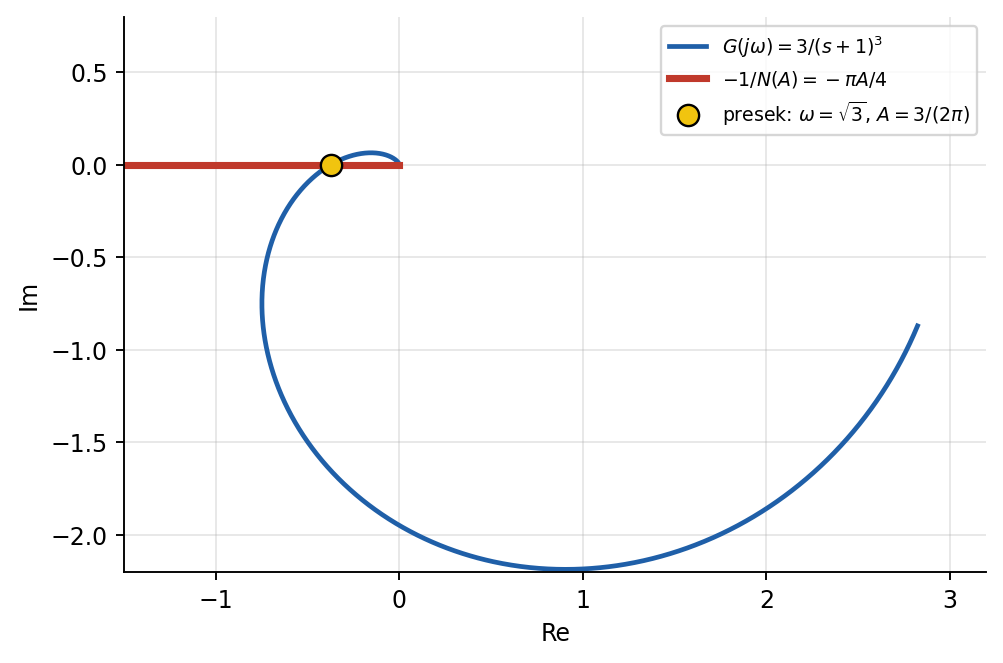
\includegraphics[width=0.6\linewidth,height=\textheight,keepaspectratio,alt={Primer sa predavanja: Nikvistova kriva 3/(s+1)³ seče negativnu realnu osu u -3/8; tu je i kritična kriva idealnog releja, pa je presek ω = √3, A = 3/(2π)}]{figures/nel_primer_relej.png}
\caption{Primer sa predavanja: Nikvistova kriva 3/(s+1)³ seče negativnu realnu osu u -3/8; tu je i kritična kriva idealnog releja, pa je presek ω = √3, A = 3/(2π)}
\end{figure}

\subsection{Stabilnost graničnog ciklusa: uopšteni Nikvistov kriterijum}

Za linearnu petlju sa pojačanjem \(K\) i stabilnim \(G(s)\), zatvorena sprega je stabilna ako Nikvistova kriva \textbf{ne obuhvata} kritičnu tačku \(-1/K\). Uopštenje: pojačanje zamenimo sa \(N(A)\), pa kritična tačka postaje \(-1/N(A)\):

\begin{itemize}
\item \(-1/N(A)\) \textbf{van} oblasti koju obuhvata Nikvistova kriva: petlja je „stabilna'', amplituda \textbf{opada};
\item \(-1/N(A)\) \textbf{unutar}: „nestabilna'', amplituda \textbf{raste};
\item \textbf{na} krivoj: oscilacija održava amplitudu (moguć granični ciklus).
\end{itemize}

\begin{kljucna}
Presek je \textbf{stabilan} granični ciklus ako se, idući duž \(-1/N(A)\) u smeru \textbf{rasta} \(A\), prelazi iz unutrašnjosti (amplituda raste) u spoljašnjost (amplituda opada). Tada svaki poremećaj vraća amplitudu na presek. U obrnutom slučaju ciklus je \textbf{nestabilan}.
\end{kljucna}

Kada nije očigledno šta je „unutra'', koristi se Raus: za zatvorenu spregu sa realnim pojačanjem \(K\) nađe se opseg \(K\) za koji je stabilna. Tačke \(-1/K\) za nestabilno \(K\) su „unutra''. Tako je rađeno u domaćem.

Pravilo važi za \textbf{stabilno} \(G(s)\) (dozvoljen je i pol u nuli, kao u domaćim zadacima). Ako \(G\) ima nestabilne polove, kritična tačka mora biti obuhvaćena odgovarajući broj puta, pa se pravilo menja (\(N = Z - P\)).

\subsection{Domaći 2.2: zadaci sa predavanja}

Za oba sistema (petlja sa \(r = 0\)) treba odrediti da li osciluje, i ako da, amplitudu i frekvenciju, pa proveriti simulacijom. Parametri nelinearnosti nisu zadati, pa se usvajaju.

\subsubsection{Zadatak 1: zasićenje i G(s) = 4/(s(s+1)²)}

Usvojeno: \(k = 1\), \(\varepsilon = 1\).

\textbf{Frekvencijski odziv} (racionalizacijom):

\[G(j\omega) = -\frac{8}{(\omega^2 + 1)^2} - j\frac{4(1 - \omega^2)}{\omega(\omega^2 + 1)^2}\]

\(\operatorname{Im}G = 0\) za \(\omega = 1\), i tada je \(G(j1) = -8/4 = -2\). Isto iz faze: \(-90° - 2\operatorname{arctg}\omega = -180°\) daje \(\omega = 1\), a \(|G(j1)| = 4/(1\cdot 2) = 2\).

\textbf{Harmonijski balans}: \(-1/N(A) = -2\), tj. \(N(A) = 1/2\). Sa \(\sin\beta = 1/A\):

\[\frac{2}{\pi}\left[\beta + \sin\beta\cos\beta\right] = \frac12\]

Numerički (npr. \texttt{fzero} u Matlabu, jer jednačina \(\beta + \sin\beta\cos\beta = \pi/4\) nema rešenje u zatvorenom obliku): \(\beta \approx 0{,}416\), pa je \(A = 1/\sin\beta \approx 2{,}48\). Provera: \(\sin0{,}416 = 0{,}404\), \(\cos0{,}416 = 0{,}915\), \((2/\pi)(0{,}416 + 0{,}370) = 0{,}500\).

\[\omega = 1\ \text{rad/s}\ (T \approx 6{,}28\ \text{s}), \qquad A \approx 2{,}48\]

\textbf{Stabilnost ciklusa.} Sa pojačanjem \(K\) karakteristični polinom je \(s^3 + 2s^2 + s + 4K\). Raus: stabilno za \(2\cdot1 > 4K\), tj. \(K < 0{,}5\). Dakle tačke \(-1/K \in (-2, 0)\) su unutra.

\begin{itemize}
\item Mala amplituda: \(N \approx 1\), \(-1/N \approx -1\), unutra, amplituda raste.
\item Posle preseka (\(A > 2{,}48\)): \(-1/N < -2\), spolja, amplituda opada.
\end{itemize}

Ciklus je \textbf{stabilan}. Pošto je \(N(A) \le k\), presek postoji samo za \(k > 0{,}5\).

\begin{figure}
\centering
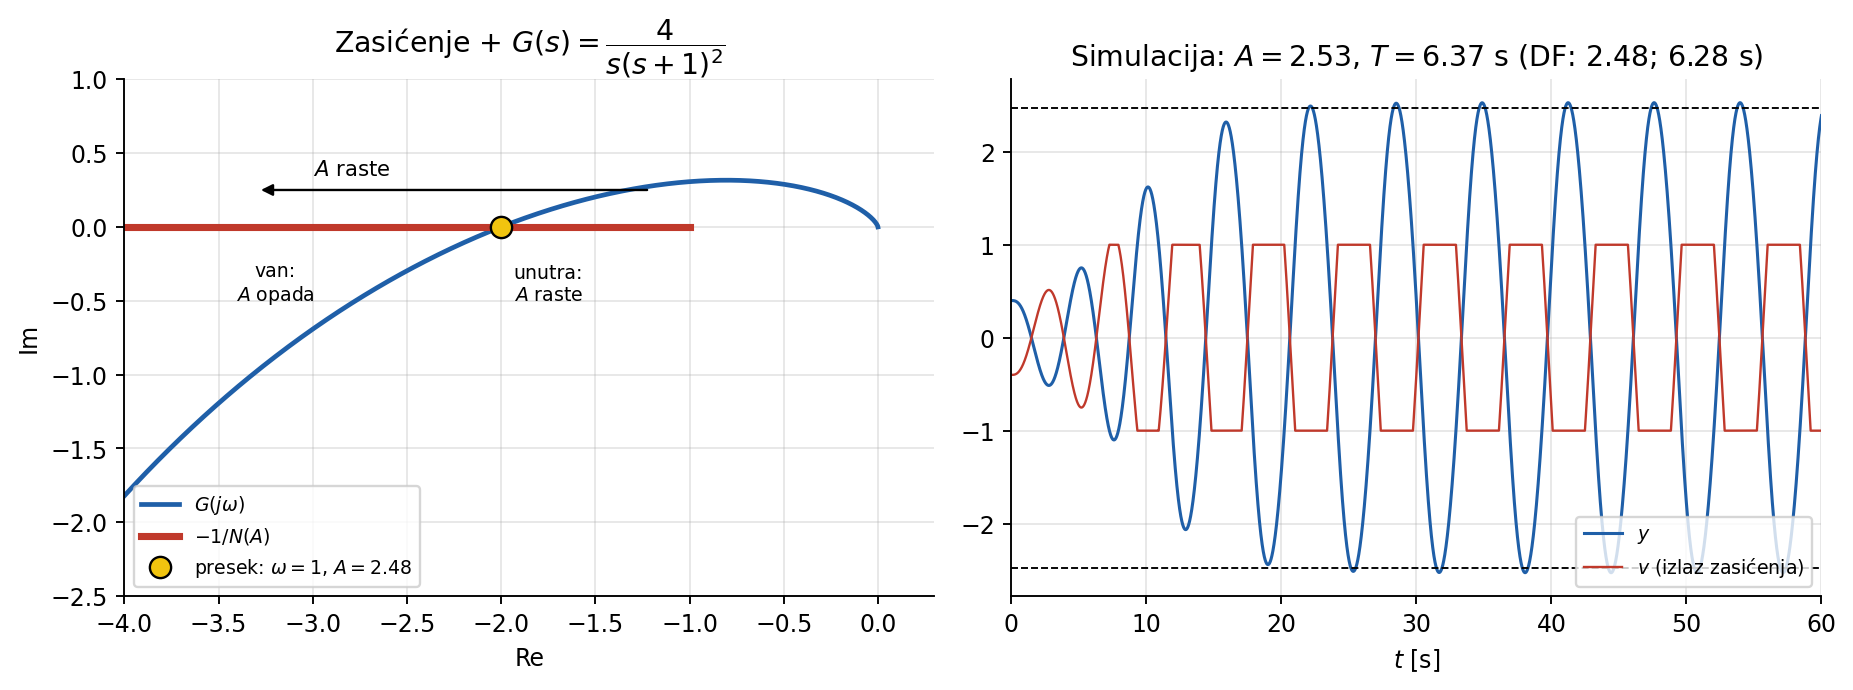
\includegraphics[width=0.95\linewidth,height=\textheight,keepaspectratio,alt={Domaći 2.2, zadatak 1: kritična kriva zasićenja (crveno) ide od -1 ulevo i seče Nikvistovu krivu u -2; simulacija daje A = 2,53 i T = 6,37 s, blizu predviđanja 2,48 i 6,28 s}]{figures/nel_zad221.png}
\caption{Domaći 2.2, zadatak 1: kritična kriva zasićenja (crveno) ide od -1 ulevo i seče Nikvistovu krivu u -2; simulacija daje A = 2,53 i T = 6,37 s, blizu predviđanja 2,48 i 6,28 s}
\end{figure}

\subsubsection{Zadatak 2: relej sa histerezisom i G(s) = 40/(s(s+2)(s+3))}

\textbf{Koja je funkcija prenosa?} Na predavanju je sa table zapisano \(\frac{40}{s(s+2)(s+3)}\). Zvanični spisak kaže samo „zadaci sa predavanja'', bez jednačina, pa se radi sa \((s+3)\). Na kraju je data i varijanta sa \((s+8)\), ako je u tekstu zadatka tako. Postupak je isti.

Usvojeno: \(K = 1\), \(\delta = 0{,}1\).

\textbf{Frekvencijski odziv}:

\[G(j\omega) = -\frac{200}{(\omega^2 + 4)(\omega^2 + 9)} - j\frac{40(6 - \omega^2)}{\omega(\omega^2 + 4)(\omega^2 + 9)}\]

Bez histerezisa presek sa realnom osom je u \(\omega = \sqrt6 \approx 2{,}45\), gde je \(G = -200/(10\cdot15) = -1{,}33\). Idealni relej bi dao \(A = \frac{4}{\pi}\cdot1{,}33 = 1{,}70\).

\textbf{Harmonijski balans sa histerezisom.} \(-1/N\) je prava \(\operatorname{Im} = -\frac{\pi\delta}{4K} = -0{,}0785\), pa se jednačina razdvaja:

\begin{enumerate}
\def\labelenumi{\arabic{enumi}.}
\item iz imaginarnog dela: \(\operatorname{Im}G(j\omega) = -0{,}0785\) daje \(\omega \approx 2{,}32\) rad/s;
\item iz realnog dela: \(\operatorname{Re}G(j2{,}32) = -200/(9{,}39\cdot14{,}39) \approx -1{,}48\), pa je \(\frac{\pi}{4K}\sqrt{A^2 - \delta^2} = 1{,}48\), tj. \(\sqrt{A^2 - \delta^2} = 1{,}886\).
\end{enumerate}

\[\omega \approx 2{,}32\ \text{rad/s}\ (T \approx 2{,}71\ \text{s}), \qquad A \approx 1{,}89\]

Histerezis (kašnjenje) \textbf{smanjuje frekvenciju} (\(2{,}32 < 2{,}45\)) i \textbf{povećava amplitudu} (\(1{,}89 > 1{,}70\)) u odnosu na idealni relej. Nije dovoljno stati na zaključku da „nelinearnost ima Im komponentu, pa se ne seče na realnoj osi''; treba izračunati presek i amplitudu, kao gore.

\textbf{Stabilnost.} Raus za \(s^3 + 5s^2 + 6s + 40K\): stabilno za \(30 > 40K\), tj. \(K < 0{,}75\), pa su tačke između \(-1{,}33\) i nule unutra. Za \(A\) malo veće od \(\delta\) tačka \(-1/N\) je blizu imaginarne ose (unutra, amplituda raste); sa rastom \(A\) ide ulevo i posle preseka je spolja (amplituda opada). Ciklus je \textbf{stabilan}.

\begin{figure}
\centering
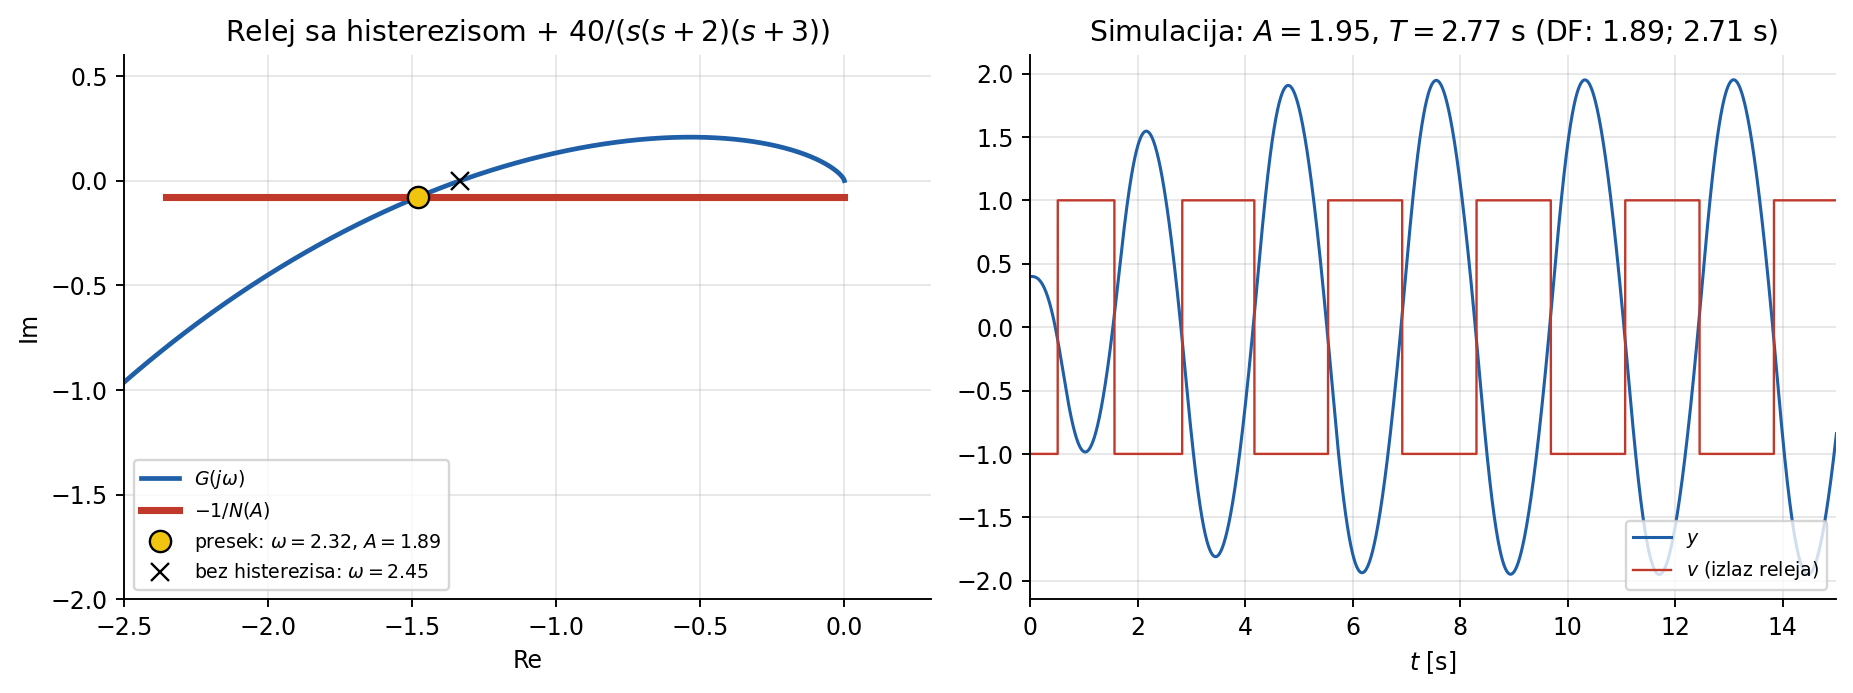
\includegraphics[width=0.95\linewidth,height=\textheight,keepaspectratio,alt={Domaći 2.2, zadatak 2 sa (s+3): prava -1/N(A) seče Nikvistovu krivu malo ispod realne ose, levo od preseka bez histerezisa (×); simulacija daje A = 1,95 i T = 2,77 s, prema predviđenim 1,89 i 2,71 s}]{figures/nel_zad222_s3.png}
\caption{Domaći 2.2, zadatak 2 sa (s+3): prava -1/N(A) seče Nikvistovu krivu malo ispod realne ose, levo od preseka bez histerezisa (×); simulacija daje A = 1,95 i T = 2,77 s, prema predviđenim 1,89 i 2,71 s}
\end{figure}

\textbf{Varijanta sa \((s+8)\)} (ako je u tekstu zadatka tako): bez histerezisa \(\omega = 4\), \(G = -0{,}25\), \(A = 0{,}32\); sa histerezisom \(\omega \approx 3{,}13\) rad/s, \(\operatorname{Re}G \approx -0{,}394\), \(A \approx 0{,}51\) (\(T \approx 2{,}0\) s). Simulacija: \(A = 0{,}53\), \(T = 2{,}05\) s. Ciklus je takođe stabilan.

\begin{figure}
\centering
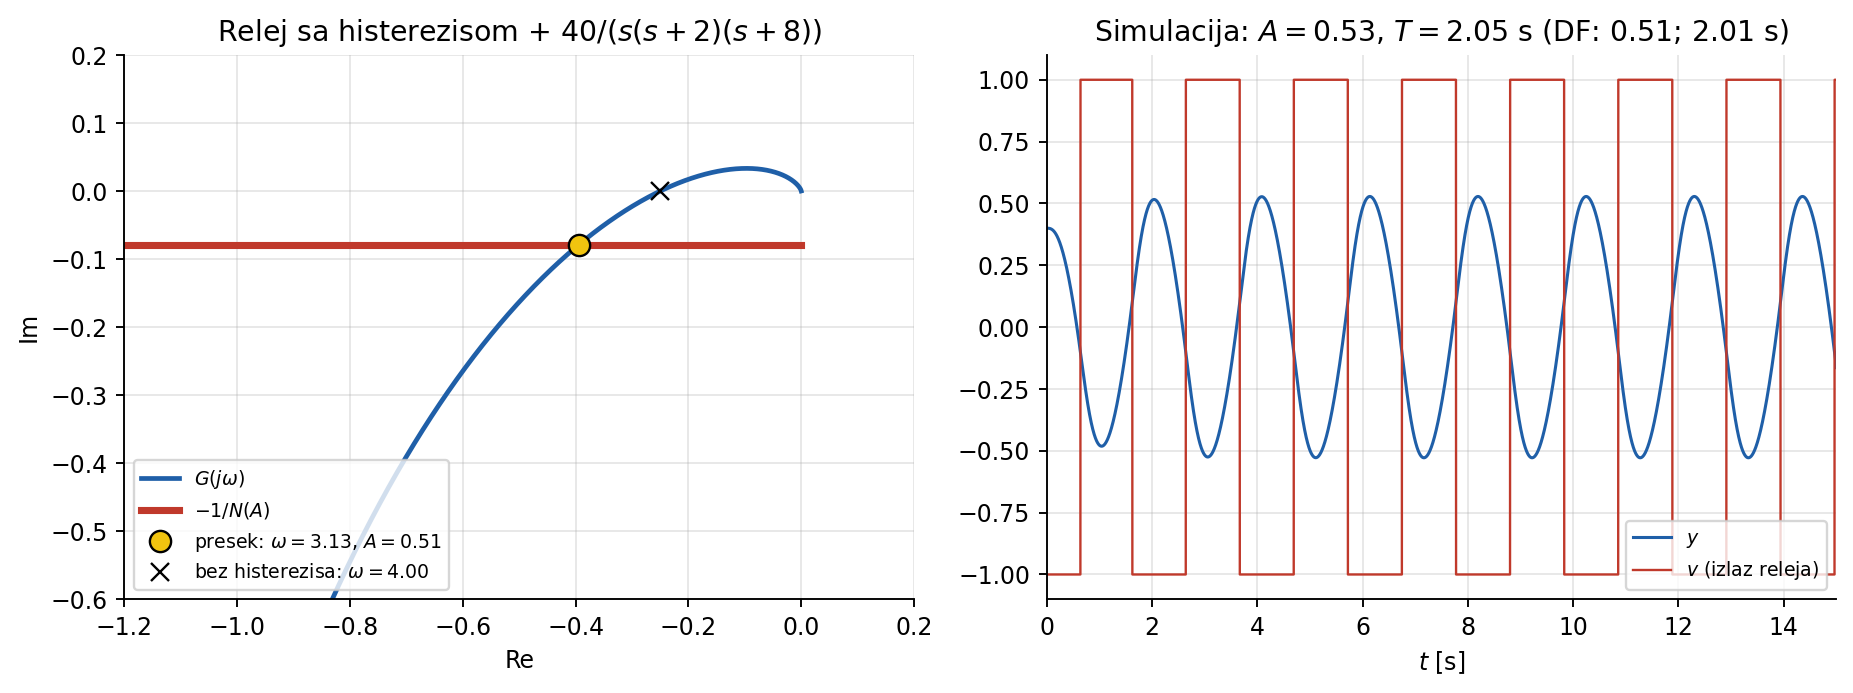
\includegraphics[width=0.95\linewidth,height=\textheight,keepaspectratio,alt={Varijanta zadatka 2 sa (s+8): isti postupak, presek kod ω = 3,13 i A = 0,51}]{figures/nel_zad222_s8.png}
\caption{Varijanta zadatka 2 sa (s+8): isti postupak, presek kod ω = 3,13 i A = 0,51}
\end{figure}

U Simulink-u: blok \textbf{Relay} sa „Switch on point'' \(= +\delta\), „Switch off point'' \(= -\delta\) i izlazom \(\pm K\), pa \(G(s)\) i negativna povratna sprega.

\subsubsection{Pitanja na odbrani (2.2)}

\begin{enumerate}
\def\labelenumi{\arabic{enumi}.}
\item \textbf{Zašto ste u zadatku 1 tražili \(\operatorname{Im}G(j\omega) = 0\)?} \(N\) zasićenja je realna, pa \(-1/N\) leži na negativnoj realnoj osi; presek je moguć samo gde Nikvistova kriva seče tu osu (faza \(-180°\)).
\item \textbf{Kako znate da je ciklus stabilan?} Idući duž \(-1/N\) u smeru rasta \(A\), tačka prelazi iz oblasti koju Nikvistova kriva obuhvata (tamo bi linearna petlja sa tim pojačanjem bila nestabilna, po Rausu) u oblast van nje; poremećaj amplitude se zato vraća na presek.
\item \textbf{Zašto simulacija daje \(A = 2{,}53\), a ne \(2{,}48\)?} Harmonijski balans je približan: zanemaren je treći harmonik, koji \(G\) guši, ali ne potpuno (\(|G(3j)|/|G(j)| \approx 1/15\)). Razlika od 2--3\% je očekivana.
\item \textbf{Šta ako promenite parametre zasićenja?} Uslov je \(k\,N_1(A/\varepsilon) = 1/2\): \(A\) raste srazmerno sa \(\varepsilon\), a raste i sa \(k\) (za \(k = 2\) je \(A \approx 5{,}06\)). Za \(k \le 0{,}5\) ciklusa nema, jer je tada petlja stabilna i za male amplitude.
\item \textbf{Zašto histerezis smanjuje frekvenciju, a povećava amplitudu?} Histerezis unosi fazno kašnjenje, pa \(G\) sme da ima manje kašnjenje od \(180°\): presek je na nižem \(\omega\), gde je \(|G|\) veće, pa je veća i amplituda.
\item \textbf{Šta ako povećate \(\delta\) ili \(K\) releja?} Prava \(-1/N\) je na \(\operatorname{Im} = -\pi\delta/(4K)\). Veće \(\delta\) je spušta: \(\delta = 0{,}3\) daje \(\omega \approx 2{,}13\), \(A \approx 2{,}22\). Veće \(K\) je podiže i skalira amplitudu: \(K = 2\) daje \(\omega \approx 2{,}38\), \(A \approx 3{,}59\).
\item \textbf{Da li relej sa histerezisom uvek daje ciklus sa ovim \(G\)?} Da: za \(\omega < \sqrt6\) imaginarni deo \(G\) ide od \(-\infty\) do 0, pa uvek seče pravu \(\operatorname{Im} = -\pi\delta/(4K)\). Kod zasićenja presek postoji tek za \(k > 0{,}5\).
\item \textbf{Kako ste iz simulacije očitali amplitudu i periodu?} Posle prelaznog procesa: amplituda kao maksimum \(|y|\) (ili \(|e|\)), perioda kao razmak između dva uzastopna prolaska kroz nulu u istom smeru.
\item \textbf{Šta ako je u zadatku 2 \((s+8)\) umesto \((s+3)\)?} Postupak je isti; treba znati rezultat za verziju koju ste zaista rešavali (za \((s+8)\): \(\omega \approx 3{,}13\) rad/s, \(A \approx 0{,}51\)).
\end{enumerate}

\subsection{Domaći 2.3: Khalil 7.11 pod 1, 2 i 3}

Petlja iz Khalil-a (slika 7.1): \(G(s)\) i statička nelinearnost \(\psi(\cdot)\) u negativnoj povratnoj sprezi, \(r = 0\). Treba ispitati postojanje periodičnih rešenja, rešiti harmonijski balans u Matlabu i simulirati.

\subsubsection{Zajedničko za pod 1 i 2: G(s) = (1 − s)/(s(s+1))}

Imenilac je \(j\omega(1 + j\omega) = -\omega^2 + j\omega\). Množenjem brojioca i imenioca konjugovanim imeniocem \(-\omega^2 - j\omega\):

\[G(j\omega) = \frac{(1 - j\omega)(-\omega^2 - j\omega)}{\omega^4 + \omega^2} = \frac{-2\omega^2 + j(\omega^3 - \omega)}{\omega^2(\omega^2 + 1)} = -\frac{2}{1 + \omega^2} - j\frac{1 - \omega^2}{\omega(1 + \omega^2)}\]

\(\operatorname{Im}G = 0\) za \(\omega = 1\), gde je \(G(j1) = -1\). Obe nelinearnosti imaju realnu \(N\), pa je uslov \(N(a) = 1\) uz \(\omega = 1\).

Sa pojačanjem \(K\): \(s(s+1) + K(1 - s) = s^2 + (1 - K)s + K\), stabilno za \(0 < K < 1\). Dakle tačke levo od \(-1\) (\(N < 1\)) su spolja, a između \(-1\) i nule (\(N > 1\)) unutra.

\subsubsection{Pod 1: ψ(y) = y⁵}

Opisna funkcija: \(a_1 = \frac{1}{\pi}\int_0^{2\pi} a^5\sin^6\theta\,d\theta\). Pošto je \(\int_0^{2\pi}\sin^6\theta\,d\theta = \frac{5\pi}{8}\), dobija se \(a_1 = \frac{5}{8}a^5\). Isto se dobija iz identiteta \(\sin^5\theta = \frac{10\sin\theta - 5\sin3\theta + \sin5\theta}{16}\), čiji je prvi harmonik \(\frac{10}{16} = \frac58\):

\[N(a) = \frac{5a^4}{8} = 1 \quad\Rightarrow\quad a = \left(\frac{8}{5}\right)^{1/4} \approx 1{,}12, \qquad \omega = 1\ \text{rad/s}\]

\textbf{Stabilnost}: \(N\) \textbf{raste} sa \(a\). Za \(a < 1{,}12\) je \(N < 1\) (spolja), pa amplituda opada; za \(a > 1{,}12\) je \(N > 1\) (unutra), pa raste. Periodično rešenje postoji, ali je \textbf{nestabilno}: to je granica oblasti privlačenja nule.

Simulacija: iz \(y(0) = 0{,}9\) izlaz se smiruje (sporo, jer je za malo \(y\) član \(y^5\) zanemarljiv), a iz \(y(0) = 1{,}3\) rešenje eksplodira za oko 0,1 s. To je konačno vreme bekstva zbog \(y^5\).

\subsubsection{Pod 2: mrtva zona + zasićenje (Khalil 7.10 pod 5)}

Neparna nelinearnost: 0 za \(|y| \le A\), nagib \(k\) između \(A\) i \(B\), zasićenje iznad \(B\); \(A = 1\), \(B = 3/2\), \(k = 2\). Opisna funkcija iz knjige:

\[\Psi(a) = \begin{cases} 0, & a \le A \\ k\left[1 - N(a/A)\right], & A \le a \le B \\ k\left[N(a/B) - N(a/A)\right], & a \ge B \end{cases}, \qquad N(x) = \frac{2}{\pi}\left[\arcsin\frac{1}{x} + \frac{1}{x}\sqrt{1 - \frac{1}{x^2}}\right]\]

\(N(x)\) je opisna funkcija jediničnog zasićenja. Zato je \(\Psi\) razlika dva zasićenja (mrtva zona = linearno minus zasićenje). Za uslov \(\Psi(a) = 1\): \(\Psi\) je 0 do \(a = 1\), raste do maksimuma \(\Psi_{max} \approx 0{,}503\) za \(a \approx 1{,}80\), pa opada ka 0. Na primer \(\Psi(2) = 2[N(4/3) - N(2)] = 2(0{,}856 - 0{,}609) = 0{,}49\).

\[\Psi(a) \le 0{,}503 < 1 \quad \forall a \quad\Rightarrow\quad \text{nema preseka, nema periodičnog rešenja}\]

Simulacija iz \(y(0) = 3\) nema oscilacija: \(y\) se zaustavi na konstanti oko \(-0{,}81\). To nije greška: za \(|y| \le 1\) nelinearnost je u mrtvoj zoni i daje nulu, a \(G\) ima integrator, pa je svaka konstanta \(|y| \le 1\) ravnoteža.

\subsubsection{Pod 3: idealni relej i G(s) = 1/(s+1)⁶}

Idealni relej \(K = 1\): \(-1/N = -\pi a/4\). Faza \(-6\operatorname{arctg}\omega = -180°\) daje \(\omega = \operatorname{tg}30° = 1/\sqrt3\). Tada

\[|G| = \frac{1}{(1 + 1/3)^3} = \frac{27}{64} \approx 0{,}422, \qquad \frac{\pi a}{4} = \frac{27}{64} \;\Rightarrow\; a = \frac{27}{16\pi} \approx 0{,}537, \qquad T \approx 10{,}9\ \text{s}\]

Kao u primeru sa predavanja, \(-1/N\) sa rastom \(a\) ide iz unutrašnjosti napolje: \textbf{stabilan} ciklus. \(1/(s+1)^6\) jako guši više harmonike, pa se simulacija skoro savršeno slaže (\(a = 0{,}544\), \(T = 10{,}88\) s).

\begin{figure}
\centering
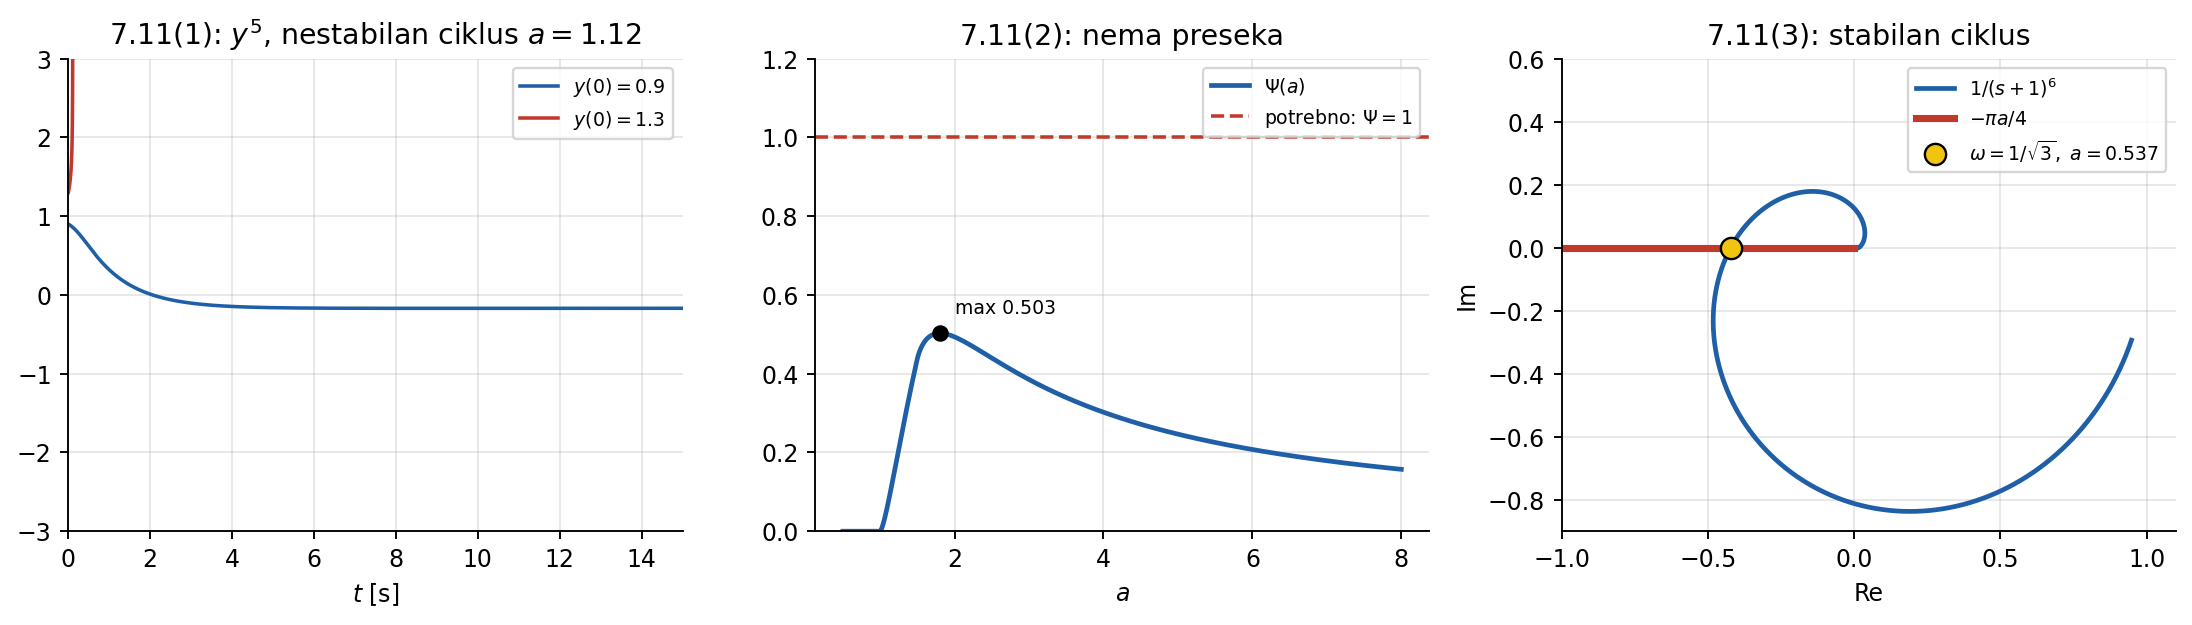
\includegraphics[width=1\linewidth,height=\textheight,keepaspectratio,alt={Domaći 2.3: (1) za y⁵ rešenje ispod ciklusa se smiruje, a iznad njega eksplodira; (2) Ψ(a) nikad ne dostiže potrebnu vrednost 1; (3) presek Nikvistove krive 1/(s+1)⁶ i kritične krive releja daje stabilan ciklus}]{figures/nel_zad23_khalil711.png}
\caption{Domaći 2.3: (1) za y⁵ rešenje ispod ciklusa se smiruje, a iznad njega eksplodira; (2) Ψ(a) nikad ne dostiže potrebnu vrednost 1; (3) presek Nikvistove krive 1/(s+1)⁶ i kritične krive releja daje stabilan ciklus}
\end{figure}

\subsubsection{Druga varijanta spiska (7.11 pod 5, 6, 7)}

Ovo je varijanta spiska iz druge godine. Kratki rezultati, za slučaj da se pojave:

\begin{longtable}[]{@{}
  >{\raggedright\arraybackslash}p{(\linewidth - 4\tabcolsep) * \real{0.0667}}
  >{\raggedright\arraybackslash}p{(\linewidth - 4\tabcolsep) * \real{0.4667}}
  >{\raggedright\arraybackslash}p{(\linewidth - 4\tabcolsep) * \real{0.4667}}@{}}
\caption{Rezultati druge varijante}\tabularnewline
\toprule\noalign{}
\begin{minipage}[b]{\linewidth}\raggedright
Pod
\end{minipage} & \begin{minipage}[b]{\linewidth}\raggedright
\(G(s)\) i nelinearnost
\end{minipage} & \begin{minipage}[b]{\linewidth}\raggedright
Rezultat
\end{minipage} \\
\midrule\noalign{}
\endfirsthead
\toprule\noalign{}
\begin{minipage}[b]{\linewidth}\raggedright
Pod
\end{minipage} & \begin{minipage}[b]{\linewidth}\raggedright
\(G(s)\) i nelinearnost
\end{minipage} & \begin{minipage}[b]{\linewidth}\raggedright
Rezultat
\end{minipage} \\
\midrule\noalign{}
\endhead
\bottomrule\noalign{}
\endlastfoot
5 & \(\frac{s}{s^2 - s + 1}\), \(y^5\) & \(\omega = 1\), \(G(j1) = -1\), \(a = (8/5)^{1/4} \approx 1{,}12\) \\
6 & \(\frac{5(s + 0{,}25)}{s^2(s+2)^2}\), \(N = 2 + \frac{4}{\pi a}\) & \(\omega = \sqrt3\), \(G = -5/12\), \(N = 2{,}4\), \(a \approx 3{,}18\) \\
7 & isto \(G\), relej sa mrtvom zonom (\(A = B = 1\)) & \(N_{max} = 2/\pi < 2{,}4\): nema preseka \\
\end{longtable}

Kod pod 5 \(G\) ima \textbf{nestabilne} polove (\(0{,}5 \pm j0{,}87\)), pa se stabilnost ciklusa ne sme čitati jednostavnim pravilom „unutra/spolja''.

\subsubsection{Pitanja na odbrani (2.3)}

\begin{enumerate}
\def\labelenumi{\arabic{enumi}.}
\item \textbf{Šta u praksi znači nestabilan ciklus u pod 1?} To je granica oblasti privlačenja nule: rešenja sa amplitudom ispod \(a \approx 1{,}12\) se smiruju, a iznad nje rastu i, zbog \(y^5\), eksplodiraju za konačno vreme.
\item \textbf{Zašto se nula smiruje iz \(y(0) = 0{,}9\), a eksplodira iz \(1{,}3\)?} Prvo je unutar oblasti privlačenja (ispod ciklusa), drugo izvan; simulacija tako potvrđuje da je ciklus nestabilan.
\item \textbf{Zašto je slaganje simulacije i predviđanja najbolje u pod 3?} \(1/(s+1)^6\) opada sa \(-120\) dB/dek i jako guši više harmonike; \(G\) iz pod 1 opada samo sa \(-20\) dB/dek, a \(y^5\) još i stvara jak peti harmonik.
\item \textbf{Zašto u pod 2 nema oscilacija i zašto \(y\) stane na \(-0{,}81\)?} \(\Psi(a) \le 0{,}503\), a za ciklus treba \(\Psi = 1\), pa preseka nema. Za \(|y| \le 1\) mrtva zona daje nulu, a \(G\) ima integrator, pa je svaka konstanta \(|y| \le 1\) ravnoteža.
\item \textbf{Kako je dobijena opisna funkcija u pod 2?} Mrtva zona sa zasićenjem je razlika dva zasićenja (sa pragovima \(B\) i \(A\)). Furijeov koeficijent je integral, a integral je linearan, pa je i \(\Psi\) razlika dve opisne funkcije zasićenja.
\item \textbf{Da li „nema preseka'' dokazuje da nema ciklusa?} Ne; harmonijski balans je približna metoda. Simulacija to ovde potvrđuje.
\item \textbf{Kako ste rešili harmonijski balans u Matlabu?} \texttt{fzero} za \(\operatorname{Im}G(j\omega) = 0\) (daje \(\omega\)), pa \texttt{fzero} za \(N(a) = -1/G(j\omega)\) (daje \(a\)); ili \texttt{fsolve} na obe realne jednačine odjednom.
\item \textbf{Šta ako promenite pojačanje releja u pod 3?} \(\omega\) se ne menja (zavisi samo od faze \(G\)), a amplituda raste srazmerno \(K\): \(a = 4K|G|/\pi\), pa za \(K = 2\) ispada \(a \approx 1{,}07\).
\item \textbf{Zašto je tačka \(-1\) granica u pod 1 i 2?} Linearna petlja sa pojačanjem \(K\) je stabilna za \(0 < K < 1\), pa je \(N = 1\) granica: \(N < 1\) znači da amplituda opada, a \(N > 1\) da raste.
\end{enumerate}

\begin{ispit}
Umeti izvesti \(N(A)\) za zasićenje i relej sa histerezisom (simetrije, granice integracije, \(\varepsilon = A\sin\beta\)), napisati jednačinu harmonijskog balansa i objasniti pretpostavke (niskopropusni \(G\), statička nelinearnost). Za svaki presek reći i da li je ciklus stabilan i zašto. Zamke: znak faze histerezisa je negativan (kašnjenje); metoda je približna; ako nema preseka, zaključak je „metoda ne predviđa ciklus''. Za zadatak 2.2/2 znati da postoje dve verzije \(G(s)\).
\end{ispit}

\section{Linearizacija u povratnoj sprezi}

Predavanja iz ove oblasti nisu snimljena niti prepisana. Teorija u ovom poglavlju je standardna, po Khalil-u (gl. 13) i Marquez-u (gl. 10) \izvor{standardna teorija, Khalil}. Domaći zadaci su upoređeni sa tri referentna rešenja.

\subsection{Ideja}

Umesto da se nelinearni sistem aproksimira linearnim oko radne tačke, upravljanje se bira tako da \textbf{tačno poništi} nelinearnost. Izlaz se diferencira dok se u izvodu ne pojavi \(u\); tada se \(u\) izrazi tako da taj izvod postane novi, proizvoljni ulaz \(v\). Izlaz se onda ponaša kao lanac integratora, a \(v\) se projektuje linearnim metodama. Cena: deo stanja može ostati „sakriven'' (unutrašnja dinamika), i on mora sam po sebi biti stabilan. To proverava \textbf{nulta dinamika}.

\subsection{Uvodni primer}

Klatno sa momentom kao ulazom: \(\dot x_1 = x_2\), \(\dot x_2 = -a\sin x_1 - bx_2 + cu\). Ako izaberemo

\[u = \frac{1}{c}\left(a\sin x_1 + v\right)\]

dobijamo \(\dot x_1 = x_2\), \(\dot x_2 = -bx_2 + v\): linearan sistem, \textbf{globalno} (ne samo oko radne tačke). Novi ulaz \(v = -k_1x_1 - k_2x_2\) ga stabilizuje. Ovde se \(u\) pojavljuje u istoj jednačini kao nelinearnost; u opštem slučaju to nije tako, pa treba sistematski postupak.

\subsection{Lijev izvod i relativni stepen}

Posmatramo sistem sa jednim ulazom i jednim izlazom, afin po upravljanju:

\[\dot x = f(x) + g(x)u, \qquad y = h(x), \qquad x \in \mathbb{R}^n\]

\textbf{Lijev izvod} funkcije \(h\) duž vektorskog polja \(f\) je izvod \(h\) duž trajektorija sistema \(\dot x = f(x)\):

\[L_fh(x) = \frac{\partial h}{\partial x}f(x), \qquad L_f^2h = L_f(L_fh), \qquad L_gL_fh = \frac{\partial(L_fh)}{\partial x}g(x)\]

Diferenciranje izlaza:

\[\dot y = \frac{\partial h}{\partial x}\left[f(x) + g(x)u\right] = L_fh(x) + L_gh(x)\,u\]

Ako je \(L_gh = 0\), u \(\dot y\) nema \(u\), pa diferenciramo ponovo: \(\ddot y = L_f^2h + L_gL_fh\,u\). I tako dalje.

\textbf{Relativni stepen} \(\rho\) je broj diferenciranja izlaza dok se \(u\) ne pojavi \izvor{standardna teorija, Khalil 13.2}:

\[L_gL_f^{i}h(x) = 0 \quad \text{za } i = 0, \dots, \rho - 2, \qquad L_gL_f^{\rho - 1}h(x) \ne 0\]

Tada je

\[y^{(\rho)} = L_f^\rho h(x) + L_gL_f^{\rho-1}h(x)\,u\]

Kada je \(\rho\) definisan, važi \(1 \le \rho \le n\). Za linearni sistem \(\rho\) je višak polova nad nulama (domaći 3.1). Relativni stepen ne zavisi od izbora koordinata stanja, jer je definisan preko veze ulaz--izlaz.

\subsection{Linearizacija ulaz--izlaz}

Iz poslednje jednačine upravljanje

\[u = \frac{1}{L_gL_f^{\rho-1}h(x)}\left[-L_f^\rho h(x) + v\right] \quad\Rightarrow\quad y^{(\rho)} = v\]

pretvara vezu od \(v\) do \(y\) u lanac od \(\rho\) integratora. Zatim se bira, na primer,

\[v = -k_0y - k_1\dot y - \dots - k_{\rho-1}y^{(\rho-1)}\]

sa koeficijentima tako da je \(s^\rho + k_{\rho-1}s^{\rho-1} + \dots + k_0\) Hurvicov polinom; tada \(y \to 0\) eksponencijalno. Za praćenje reference \(y_r(t)\) uzima se \(v = y_r^{(\rho)} - \sum k_i(y^{(i)} - y_r^{(i)})\).

U oznakama iz Khalil-a: \(\gamma(x) = L_gL_f^{\rho-1}h\), \(\alpha(x) = -L_f^\rho h/\gamma\), pa je \(u = \alpha(x) + \gamma^{-1}(x)v\).

\begin{zasto}
Zašto ovo ne rešava sve: izlaz „vidi'' samo \(\rho\) stanja (\(y, \dot y, \dots, y^{(\rho-1)}\)). Ako je \(\rho < n\), ostalih \(n - \rho\) stanja se ne vidi na izlazu. Upravljanje koje drži \(y\) na nuli može ih pustiti da divergiraju. Zato se sistem prepisuje u normalnu formu.
\end{zasto}

\subsection{Normalna forma}

Uvodimo nove koordinate \izvor{standardna teorija, Khalil 13.2}:

\[z = T(x) = \begin{bmatrix} \eta \\ \xi \end{bmatrix}, \qquad \xi = \begin{bmatrix} h(x) \\ L_fh(x) \\ \vdots \\ L_f^{\rho-1}h(x) \end{bmatrix} = \begin{bmatrix} y \\ \dot y \\ \vdots \\ y^{(\rho-1)} \end{bmatrix}, \qquad \eta = \phi(x) \in \mathbb{R}^{n-\rho}\]

Funkcije \(\phi\) se biraju tako da:

\begin{enumerate}
\def\labelenumi{\arabic{enumi}.}
\item \(T\) bude \textbf{difeomorfizam} (invertibilan, glatka inverzija), bar u oblasti od interesa; proverava se da je Jakobijan \(\partial T/\partial x\) nesingularan;
\item \(\dot\eta\) \textbf{ne zavisi od \(u\)} (tada je nulta dinamika dobro definisana, bez obzira na \(u\)), tj.
  \[\frac{\partial\phi}{\partial x}\,g(x) = 0\]
\end{enumerate}

Khalil pokazuje da takve funkcije \(\phi\) lokalno uvek postoje kada je \(\rho\) definisan; u zadacima se obično pogode (kao u 3.3) ili se uzmu neka od originalnih stanja (kao u 3.1).

U novim koordinatama sistem ima oblik:

\[
\begin{aligned}
\dot\eta &= f_0(\eta, \xi) \\
\dot\xi_i &= \xi_{i+1}, \quad i = 1, \dots, \rho - 1 \\
\dot\xi_\rho &= L_f^\rho h + L_gL_f^{\rho-1}h\,u \\
y &= \xi_1
\end{aligned}
\]

\begin{itemize}
\item \(\xi\) je \textbf{spoljašnja} dinamika: lanac integratora koji se linearizuje upravljanjem.
\item \(\eta\) je \textbf{unutrašnja} (skrivena) dinamika: na nju \(u\) ne deluje direktno, već samo preko \(\xi\).
\end{itemize}

\subsection{Nulta dinamika i minimalna faza}

\textbf{Nulta dinamika} je unutrašnja dinamika kada se izlaz drži identički na nuli. Iz \(y \equiv 0\) slede i svi izvodi nula, pa je \(\xi = 0\) (upravljanje koje to obezbeđuje je \(u = -L_f^\rho h/L_gL_f^{\rho-1}h\)), i ostaje:

\[\dot\eta = f_0(\eta, 0)\]

\begin{kljucna}
Sistem je \textbf{minimalne faze} ako nulta dinamika ima \textbf{asimptotski stabilnu} ravnotežu u nuli (globalno minimalne faze, ako je GAS). Tada linearizacija ulaz--izlaz sa stabilizujućim \(v\) stabilizuje i ceo sistem (lokalno). Ako je nulta dinamika nestabilna, sistem nije minimalne faze i ovaj zakon upravljanja se ne sme koristiti.
\end{kljucna}

Naziv dolazi iz linearnih sistema: nulta dinamika linearnog sistema ima svojstvene vrednosti jednake \textbf{nulama} funkcije prenosa (domaći 3.1), a linearni sistem je minimalne faze kada su sve nule u levoj poluravni.

Nulta dinamika se u praksi često dobija i \textbf{bez} normalne forme: postavi se \(y \equiv 0\), \(\dot y \equiv 0\), ..., iz \(y^{(\rho)} = 0\) se izrazi \(u\), i to se uvrsti u preostale jednačine (tako se radi i u referentnim rešenjima zadatka 3.2).

Specijalan slučaj \(\rho = n\): nema unutrašnje dinamike, pa se ceo sistem linearizuje (linearizacija ulaz--stanje).

\subsection{Domaći 3.1: linearni sistem zadat funkcijom prenosa}

\[H(s) = \frac{b_ms^m + b_{m-1}s^{m-1} + \dots + b_1s + b_0}{s^n + a_{n-1}s^{n-1} + \dots + a_1s + a_0}, \qquad n > m, \quad b_m \ne 0\]

\begin{enumerate}
\def\labelenumi{(\alph{enumi})}
\item prostor stanja; (b) relativni stepen; (c) normalna forma, nulta dinamika, uslov minimalne faze. Uputstvo iz spiska: Khalil primer 13.4 i str. 513--515, Marquez primeri 10.16 i 10.17.
\end{enumerate}

\subsubsection{a) Prostor stanja}

Uvodimo pomoćni signal \(Z(s)\):

\[U(s) = \left(s^n + a_{n-1}s^{n-1} + \dots + a_0\right)Z(s), \qquad Y(s) = \left(b_ms^m + \dots + b_0\right)Z(s)\]

U vremenskom domenu \(u = z^{(n)} + a_{n-1}z^{(n-1)} + \dots + a_0z\) i \(y = b_mz^{(m)} + \dots + b_0z\). Sa stanjima \(x_1 = z\), \(x_2 = \dot z\), ..., \(x_n = z^{(n-1)}\) dobija se \textbf{kontrolabilna kanonska forma}:

\[
A = \begin{bmatrix}
0 & 1 & 0 & \cdots & 0 \\
0 & 0 & 1 & \cdots & 0 \\
\vdots & & & \ddots & \vdots \\
0 & 0 & 0 & \cdots & 1 \\
-a_0 & -a_1 & -a_2 & \cdots & -a_{n-1}
\end{bmatrix}, \quad
B = \begin{bmatrix} 0 \\ 0 \\ \vdots \\ 0 \\ 1 \end{bmatrix}, \quad
C = \begin{bmatrix} b_0 & b_1 & \cdots & b_m & 0 & \cdots & 0 \end{bmatrix}
\]

\(C\) ima \(m + 1\) koeficijenata i \(n - m - 1\) nula.

\subsubsection{b) Relativni stepen}

Za linearni sistem \(L_fh = CAx\), \(L_gh = CB\), i uopšte \(y^{(i)} = CA^ix + CA^{i-1}Bu\) dok su raniji članovi uz \(u\) nula. Treba naći prvo \(i\) za koje je \(CA^{i}B \ne 0\).

Ključna osobina: za vrstu \(r = [r_1, \dots, r_n]\) sa \(r_n = 0\) važi \(rA = [0, r_1, \dots, r_{n-1}]\) (poslednja vrsta od \(A\) se množi sa \(r_n = 0\), a ostale jedinice pomeraju elemente za jedno mesto udesno). Zato:

\[CA^i = \begin{bmatrix} \underbrace{0 \ \cdots\ 0}_{i} & b_0 & \cdots & b_m & 0 & \cdots & 0 \end{bmatrix}\]

sve dok \(b_m\) ne stigne na poslednje mesto. \(CA^iB\) je poslednji element vrste \(CA^i\). On je nula dok je \(b_m\) na mestu \(m + 1 + i < n\), a prvi put je \(b_m\) kada je \(m + 1 + i = n\), tj. \(i = n - m - 1\). Dakle \(u\) se prvi put javlja u izvodu reda \(n - m\):

\begin{kljucna}
\[\rho = n - m\]
Relativni stepen linearnog sistema je višak polova nad nulama.
\end{kljucna}

Primer (\(n = 6\), \(m = 3\)): \(y = b_3x_4 + \dots + b_0x_1\), \(\dot y = b_3x_5 + \dots\), \(\ddot y = b_3x_6 + \dots\), a tek \(y^{(3)}\) sadrži \(\dot x_6\), tj. \(u\). Dakle \(\rho = 3 = 6 - 3\).

\subsubsection{c) Normalna forma i nulta dinamika}

Koordinate:

\[\xi_1 = y = b_0x_1 + \dots + b_mx_{m+1}, \quad \xi_2 = \dot y = b_0x_2 + \dots + b_mx_{m+2}, \quad \dots, \quad \xi_\rho = b_0x_\rho + \dots + b_mx_n\]

\[\eta = [x_1, x_2, \dots, x_m]^T\]

Transformacija je trougaona sa \(b_m \ne 0\) na dijagonali, pa je invertibilna. \(\dot\eta\) ne zavisi od \(u\), jer \(u\) ulazi samo u \(\dot x_n\), a \(n > m\).

Jednačine za \(\eta\): \(\dot\eta_i = \eta_{i+1}\) za \(i < m\), a iz \(\xi_1 = b_0\eta_1 + \dots + b_{m-1}\eta_m + b_mx_{m+1}\):

\[\dot\eta_m = x_{m+1} = \frac{1}{b_m}\left(\xi_1 - b_0\eta_1 - \dots - b_{m-1}\eta_m\right)\]

Dakle \(\dot\eta = A_0\eta + B_0\xi_1\), sa

\[
A_0 = \begin{bmatrix}
0 & 1 & \cdots & 0 \\
\vdots & & \ddots & \vdots \\
0 & 0 & \cdots & 1 \\
-\frac{b_0}{b_m} & -\frac{b_1}{b_m} & \cdots & -\frac{b_{m-1}}{b_m}
\end{bmatrix}, \qquad
B_0 = \begin{bmatrix} 0 \\ \vdots \\ 0 \\ \frac{1}{b_m} \end{bmatrix}
\]

a spoljašnji deo je \(\dot\xi_i = \xi_{i+1}\), \(\dot\xi_\rho = CA^\rho x + b_mu\).

\textbf{Nulta dinamika} (\(\xi = 0\)): \(\dot\eta = A_0\eta\). \(A_0\) je u kompanjon formi, pa je

\[\det(sI - A_0) = s^m + \frac{b_{m-1}}{b_m}s^{m-1} + \dots + \frac{b_0}{b_m} = \frac{b(s)}{b_m}\]

Svojstvene vrednosti nulte dinamike su \textbf{nule} \(H(s)\). Kraći put do istog: \(y = 0\) znači \(b_0x_1 + b_1\dot x_1 + \dots + b_mx_1^{(m)} = 0\) (jer je \(x_{i+1} = x_1^{(i)}\)), a karakteristični polinom ove diferencijalne jednačine je brojilac \(b(s)\).

\begin{kljucna}
Sistem je minimalne faze ako i samo ako su sve nule \(H(s)\) (koreni \(b_ms^m + \dots + b_0\)) u levoj poluravni.
\end{kljucna}

\subsubsection{Pitanja na odbrani (3.1)}

\begin{enumerate}
\def\labelenumi{\arabic{enumi}.}
\item \textbf{Intuitivno, zašto je \(\rho = n - m\)?} Na visokim frekvencijama \(H(s) \approx b_m/s^{n-m}\), tj. od \(u\) do \(y\) je lanac od \(n - m\) integratora; \(u\) se zato pojavi tek u \((n - m)\)-tom izvodu izlaza.
\item \textbf{Zašto su svojstvene vrednosti nulte dinamike baš nule \(H(s)\)?} Nula prenosa je „frekvencija'' \(e^{zt}\) koju sistem može da ima iznutra, a da je izlaz identički nula. Upravo to opisuje nulta dinamika (\(y \equiv 0\)).
\item \textbf{Zašto je minimalna faza važna za ovaj zakon upravljanja?} Linearizujuće upravljanje „skraćuje'' nule: polovi zatvorene sprege koji se ne vide na izlazu dolaze na mesta nula. Nula u desnoj poluravni daje skriveni nestabilni mod: \(y \to 0\), a unutrašnja stanja divergiraju.
\item \textbf{Zašto se traži \(\frac{\partial\phi}{\partial x}g = 0\)?} Da \(u\) ne ulazi u \(\dot\eta\); tada je unutrašnja dinamika pogođena samo preko \(\xi\), i za \(\xi = 0\) dobija se nulta dinamika nezavisna od upravljanja. U 3.1 to važi jer \(u\) ulazi samo u \(\dot x_n\), a \(\eta = (x_1, \dots, x_m)\).
\item \textbf{Šta je difeomorfizam i zašto je potreban?} Glatka invertibilna promena koordinata sa glatkom inverzijom. Obezbeđuje da normalna forma opisuje isti sistem, pa se zaključci o stabilnosti prenose nazad na \(x\).
\item \textbf{Zašto kontrolabilna kanonska forma? Da li bi druga realizacija dala drugo \(\rho\)?} Ne; \(\rho\) je osobina veze \(u \to y\). Kanonska forma je izabrana jer se u njoj izvodi \(y\) računaju pomeranjem koeficijenata (\(CA^i\)).
\item \textbf{Kakvo \(u\) drži \(y \equiv 0\)?} Ono koje poništava \(y^{(\rho)}\): \(u = -CA^\rho x/b_m\) (uz \(\xi = 0\)); pod njim se stanja kreću po nultoj dinamici \(\dot\eta = A_0\eta\).
\item \textbf{Šta ako je \(m = n - 1\)?} Tada je \(\rho = 1\): već \(\dot y\) sadrži \(u\), a nulta dinamika je reda \(n - 1\).
\end{enumerate}

\subsection{Domaći 3.2: relativni stepen i nulta dinamika}

\subsubsection{Sistem 1}

\[\dot x_1 = \operatorname{tg}x_1 + x_2, \qquad \dot x_2 = x_1 + u, \qquad y = x_2\]

\textbf{Relativni stepen}: \(\dot y = \dot x_2 = x_1 + u\), pa je \(\rho = 1\). Linearizujuće upravljanje: \(u = -x_1 + v\), pa je \(\dot y = v\).

\textbf{Nulta dinamika}: \(y \equiv 0\) znači \(x_2 \equiv 0\); iz \(\dot y = 0\) je \(u = -x_1\). Ostaje

\[\dot x_1 = \operatorname{tg}x_1\]

Tri načina da se pokaže nestabilnost (svi daju isto):

\begin{itemize}
\item linearizacija: \(\operatorname{tg}x_1 \approx x_1\), pa je \(\dot x_1 = x_1\), svojstvena vrednost \(+1\);
\item \(V = \frac12x_1^2\): \(\dot V = x_1\operatorname{tg}x_1 > 0\) za \(0 < |x_1| < \pi/2\), „energija'' raste, pa je po teoremi Četajeva nula nestabilna;
\item eksplicitno rešenje: \(\frac{\cos x_1}{\sin x_1}dx_1 = dt\), pa je \(\ln|\sin x_1| = t + C\), tj. \(\sin x_1 = C_1e^t\). Desna strana raste, pa \(x_1\) za \textbf{konačno} vreme stiže do \(\pm\pi/2\), gde \(\operatorname{tg}x_1 \to \infty\).
\end{itemize}

Nulta dinamika je nestabilna, pa sistem \textbf{nije minimalne faze}. Sva tri izvora se slažu.

\subsubsection{Sistem 2}

\[\dot x_1 = -x_1 + x_2 - x_3, \qquad \dot x_2 = -x_1x_3 - x_2 + u, \qquad \dot x_3 = -x_1 + u, \qquad y = x_3\]

\textbf{Relativni stepen}: \(\dot y = \dot x_3 = -x_1 + u\), pa je \(\rho = 1\).

\textbf{Nulta dinamika}: \(y = x_3 \equiv 0\), a iz \(\dot y = 0\) sledi \(u = x_1\). Uvrstimo \(x_3 = 0\) i \(u = x_1\) u prve dve jednačine:

\[\dot x_1 = -x_1 + x_2, \qquad \dot x_2 = x_1 - x_2, \qquad A_0 = \begin{bmatrix} -1 & 1 \\ 1 & -1 \end{bmatrix}\]

\(\det(\lambda I - A_0) = (\lambda + 1)^2 - 1 = \lambda(\lambda + 2)\), pa je \(\lambda_1 = 0\), \(\lambda_2 = -2\). Šta to znači vidi se iz zbira i razlike:

\[\frac{d}{dt}(x_1 + x_2) = 0, \qquad \frac{d}{dt}(x_1 - x_2) = -2(x_1 - x_2)\]

Zbir ostaje konstantan, a razlika eksponencijalno nestaje. Trajektorije završavaju na pravoj \(x_1 = x_2 = \frac{x_1(0) + x_2(0)}{2}\), \textbf{ne u nuli}. Ljapunov potvrđuje: za \(V = \frac12(x_1^2 + x_2^2)\) je \(\dot V = -(x_1 - x_2)^2 \le 0\). To je slučaj „jedna svojstvena vrednost nula'' iz faznih portreta: cela prava ravnoteža.

\textbf{Česta greška u zaključku:} iz „granično stabilno'' zaključiti ili „sistem minimalne faze'' ili „nestabilna nulta dinamika''. Oba su pogrešna.

\textbf{Razrešenje.} Po definiciji (Khalil) minimalna faza traži \textbf{asimptotski} stabilnu nultu dinamiku. Ovde nulta dinamika jeste stabilna (rešenja su ograničena, \(\dot V \le 0\)), ali nije asimptotski stabilna (\(\lambda = 0\), zbir \(x_1 + x_2\) se ne vraća na nulu). Dakle:

\begin{itemize}
\item zaključak „nestabilna'' nije tačan: ništa ne divergira;
\item zaključak „minimalne faze'' ne važi po strogoj definiciji;
\item tačno je: nulta dinamika je stabilna po Ljapunovu, ali ne asimptotski, pa sistem \textbf{nije minimalne faze} u strogom smislu; na granici je (\emph{weakly minimum phase}, „slabo minimalne faze'').
\end{itemize}

Praktična posledica: pri upravljanju \(u = x_1 + v\) koje drži \(y\) na nuli, unutrašnja stanja ostaju ograničena, ali ne idu u nulu. Svaki poremećaj trajno pomeri zbir \(x_1 + x_2\) (ponaša se kao integrator).

\subsubsection{Pitanja na odbrani (3.2)}

\begin{enumerate}
\def\labelenumi{\arabic{enumi}.}
\item \textbf{Kako ste odredili relativni stepen?} Diferencirao sam izlaz dok se \(u\) nije pojavio sa koeficijentom različitim od nule; u oba sistema to je već prvi izvod, pa je \(\rho = 1\).
\item \textbf{Šta znači \(\rho = 1\) uz \(n = 2\) ili \(n = 3\)?} Izlaz „vidi'' jedno stanje; unutrašnja dinamika je reda \(n - 1\) i na nju upravljanje utiče samo posredno.
\item \textbf{Zašto je nulta dinamika sistema 1 nestabilna i šta se dešava u praksi?} \(\dot x_1 = \operatorname{tg}x_1\) ima \(\lambda = +1\) u nuli (i \(\dot V > 0\), Četajev). Ako se primeni \(u = -x_1 + v\) sa stabilizujućim \(v\), \(y \to 0\), ali \(x_1\) za konačno vreme stigne do \(\pm\pi/2\), gde \(\operatorname{tg}x_1\) eksplodira; upravljanje je neupotrebljivo.
\item \textbf{Sistem 2: stabilan ili ne? Minimalne faze ili ne?} Nulta dinamika je stabilna (rešenja ograničena), ali ne asimptotski (\(\lambda = 0\)): stanja završe na pravoj \(x_1 = x_2\), ne u nuli. Po Khalilovoj definiciji sistem \textbf{nije} minimalne faze (na granici je).
\item \textbf{Smete li u sistemu 2 da zaključujete iz svojstvenih vrednosti kad je jedna nula?} Ovde da, jer je nulta dinamika \textbf{tačno} linearna (nije linearizacija); za nelinearnu nultu dinamiku \(\lambda = 0\) ne bi dala zaključak.
\item \textbf{Šta se praktično dešava sa \(x_1 + x_2\) u sistemu 2?} Ponaša se kao integrator: ne raste sam, ali svaki poremećaj ga trajno pomeri, jer ga ništa ne vraća na nulu.
\item \textbf{Da li nulta dinamika zavisi od izbora izlaza?} Da. Minimalna faza je osobina para sistem--izlaz: sa drugim \(y\) se menjaju i \(\rho\) i nulta dinamika.
\item \textbf{Zašto ni „minimalne faze'' ni „nestabilna''?} To su česte greške. Po strogoj definiciji (asimptotska stabilnost nulte dinamike) nulta dinamika je stabilna, ne asimptotski, pa sistem nije minimalne faze; a nije ni nestabilna, jer ništa ne divergira.
\end{enumerate}

\subsection{Domaći 3.3: normalna forma uz zadato preslikavanje}

\[
\begin{aligned}
\dot x_1 &= x_2 + x_1x_2 - x_2^2 + u \\
\dot x_2 &= x_1x_2 - x_2^2 + u \\
\dot x_3 &= x_1 + x_1x_2 - x_2^2 - (x_3 - x_1)^3 + u \\
y &= x_1 - x_2
\end{aligned}
\]

Ovde je \(g = [1, 1, 1]^T\). (a) relativni stepen; (b) normalna forma uz \(\phi(x) = x_1 - x_3\); (c) minimalna faza.

\subsubsection{a) Relativni stepen}

\[\dot y = \dot x_1 - \dot x_2 = (x_2 + x_1x_2 - x_2^2 + u) - (x_1x_2 - x_2^2 + u) = x_2\]

\(u\) se skratio, pa diferenciramo još jednom:

\[\ddot y = \dot x_2 = x_1x_2 - x_2^2 + u\]

Koeficijent uz \(u\) je 1, pa je \(\rho = 2\). Kako je \(n = 3\), postoji jedna promenljiva unutrašnje dinamike.

\subsubsection{b) Normalna forma}

Koordinate:

\[\eta = \phi(x) = x_1 - x_3, \qquad \xi_1 = y = x_1 - x_2, \qquad \xi_2 = \dot y = x_2\]

\textbf{Zašto baš ovo \(\phi\)}: uslov \(\frac{\partial\phi}{\partial x}g = 0\) daje \([1,\ 0,\ -1]\cdot[1,\ 1,\ 1]^T = 1 - 1 = 0\). Zato se u \(\dot\eta\) upravljanje skraćuje.

\textbf{Difeomorfizam}: \(T(x) = [x_1 - x_3,\ x_1 - x_2,\ x_2]^T\) je linearno, sa

\[\det\frac{\partial T}{\partial x} = \det\begin{bmatrix} 1 & 0 & -1 \\ 1 & -1 & 0 \\ 0 & 1 & 0 \end{bmatrix} = -1 \ne 0\]

pa je globalni difeomorfizam. Inverzija: \(x_2 = \xi_2\), \(x_1 = \xi_1 + \xi_2\), \(x_3 = \xi_1 + \xi_2 - \eta\).

\textbf{Jednačina za \(\eta\)}:

\[\dot\eta = \dot x_1 - \dot x_3 = (x_2 + x_1x_2 - x_2^2 + u) - (x_1 + x_1x_2 - x_2^2 - (x_3 - x_1)^3 + u) = x_2 - x_1 + (x_3 - x_1)^3\]

Pošto je \(x_2 - x_1 = -\xi_1\) i \(x_3 - x_1 = -\eta\), dobija se \(\dot\eta = -\xi_1 - \eta^3\).

\textbf{Jednačine za \(\xi\)}: \(\dot\xi_1 = \xi_2\), a

\[\dot\xi_2 = x_1x_2 - x_2^2 + u = x_2(x_1 - x_2) + u = \xi_2\xi_1 + u\]

\begin{kljucna}
Normalna forma:
\[\dot\eta = -\eta^3 - \xi_1, \qquad \dot\xi_1 = \xi_2, \qquad \dot\xi_2 = \xi_1\xi_2 + u, \qquad y = \xi_1\]
\end{kljucna}

Referentna rešenja dobijaju isto. (U jednom je u postavci greškom eksponent 2 umesto 3, ali račun koristi 3.)

\subsubsection{c) Minimalna faza}

Nulta dinamika (\(\xi = 0\)):

\[\dot\eta = -\eta^3\]

Linearizacija daje \(\dot\eta \approx 0\), svojstvenu vrednost nula, pa \textbf{ne daje zaključak}. Zato Ljapunov: \(V = \frac12\eta^2\),

\[\dot V = \eta\dot\eta = -\eta^4 < 0 \quad (\eta \ne 0)\]

\(V\) je radijalno neograničena, pa je nulta dinamika \textbf{globalno asimptotski stabilna}, i sistem \textbf{jeste minimalne faze}. Isto se dobija eksplicitnim rešenjem: \(-\frac{d\eta}{\eta^3} = dt\) daje \(\frac{1}{2\eta^2} = t + c\), tj. \(\eta^2 = \frac{1}{2(t + c)} \to 0\). Konvergencija je spora (kao \(1/\sqrt t\)), dakle asimptotska, ali ne eksponencijalna.

\textbf{Upravljanje} (dopuna, nije traženo): \(u = -\xi_1\xi_2 + v\), \(v = -2\xi_1 - 3\xi_2\) daje \(\ddot y + 3\dot y + 2y = 0\) (polovi \(-1\) i \(-2\)). Tada \(\xi \to 0\) eksponencijalno, a \(\eta\) prati nultu dinamiku.

\begin{figure}
\centering
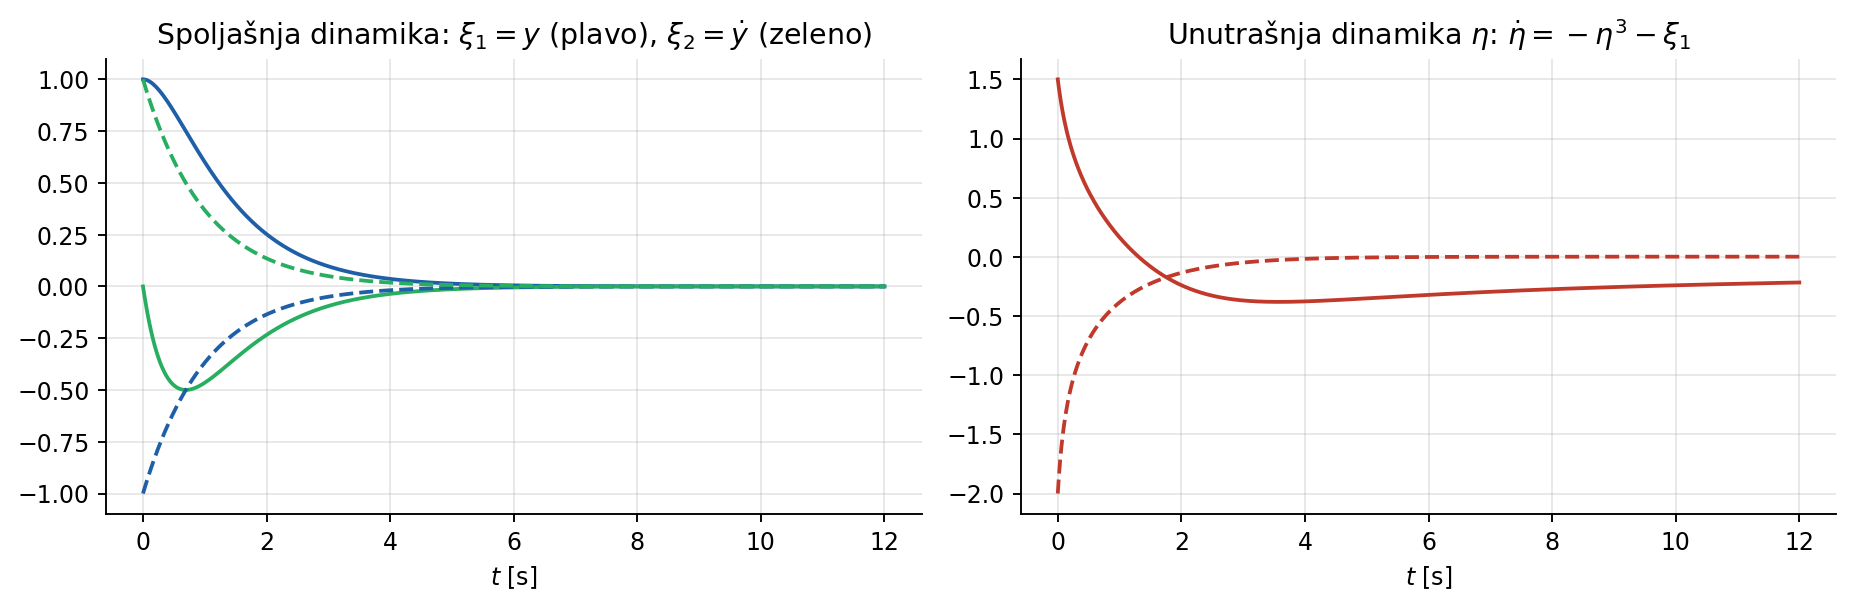
\includegraphics[width=0.95\linewidth,height=\textheight,keepaspectratio,alt={Zadatak 3.3 u zatvorenoj sprezi, dva početna stanja: spoljašnja stanja (levo) opadaju eksponencijalno kao kod linearnog sistema; unutrašnje stanje (desno) takođe teži nuli, ali sporo, jer je nulta dinamika η̇ = −η³ asimptotski, a ne eksponencijalno stabilna}]{figures/nel_fl_zad33.png}
\caption{Zadatak 3.3 u zatvorenoj sprezi, dva početna stanja: spoljašnja stanja (levo) opadaju eksponencijalno kao kod linearnog sistema; unutrašnje stanje (desno) takođe teži nuli, ali sporo, jer je nulta dinamika η̇ = −η³ asimptotski, a ne eksponencijalno stabilna}
\end{figure}

\subsubsection{Pitanja na odbrani (3.3)}

\begin{enumerate}
\def\labelenumi{\arabic{enumi}.}
\item \textbf{Zašto je \(\rho = 2\)?} U \(\dot y = \dot x_1 - \dot x_2\) se \(u\) skrati (oba stanja imaju \(+u\)), a u \(\ddot y = \dot x_2\) se pojavi sa koeficijentom 1.
\item \textbf{Kako znate da je \(\phi = x_1 - x_3\) dobar izbor?} \(\frac{\partial\phi}{\partial x}g = 1 - 1 = 0\), pa \(u\) ne ulazi u \(\dot\eta\), a Jakobijan transformacije ima determinantu \(-1 \ne 0\), pa je to globalni difeomorfizam.
\item \textbf{Da li bi drugo \(\phi\) dalo drugu nultu dinamiku?} Ne. Na primer \(\phi = x_2 - x_3\) takođe zadovoljava oba uslova (determinanta \(-1\)) i razlikuje se od \(x_1 - x_3\) za \(-\xi_1\), pa se za \(\xi = 0\) dobija ista jednačina \(\dot\eta = -\eta^3\).
\item \textbf{Zašto linearizacija ne daje zaključak za \(\dot\eta = -\eta^3\)?} Jakobijan u nuli je \(-3\eta^2|_0 = 0\): svojstvena vrednost na imaginarnoj osi, slučaj u kome indirektna metoda ne odlučuje.
\item \textbf{Zašto je stabilnost globalna?} \(V = \frac12\eta^2\) je radijalno neograničena, a \(\dot V = -\eta^4\) negativno definitna na celoj pravoj.
\item \textbf{Šta pokazuje slika zatvorene sprege?} \(\xi\) opada eksponencijalno (linearni lanac sa polovima \(-1\), \(-2\)), a \(\eta\) sporo, kao \(1/\sqrt t\): asimptotska, ali ne eksponencijalna stabilnost nulte dinamike.
\item \textbf{Šta bi bilo da je u \(\dot x_3\) član \(+(x_3 - x_1)^3\)?} Nulta dinamika bi bila \(\dot\eta = \eta^3\), nestabilna (čak konačno vreme bekstva), pa sistem ne bi bio minimalne faze i linearizujući zakon se ne bi smeo koristiti.
\item \textbf{Kako biste projektovali upravljanje?} \(u = -\xi_1\xi_2 + v\) poništava nelinearnost u \(\dot\xi_2\), a \(v = -2\xi_1 - 3\xi_2\) postavlja polove \(-1\) i \(-2\); stabilnost celog sistema sledi iz minimalne faze.
\end{enumerate}

\begin{ispit}
Postupak u tri koraka: (1) diferencirati \(y\) dok se ne pojavi \(u\), pa je broj koraka \(\rho\); (2) \(\xi = (y, \dots, y^{(\rho-1)})\) plus \(\eta\) sa \(\frac{\partial\phi}{\partial x}g = 0\), proveriti Jakobijan transformacije; (3) nulta dinamika iz \(\xi = 0\) i ispitivanje stabilnosti (ako linearizacija daje nulu, koristiti Ljapunova). Zamka: stabilna, ali ne asimptotski stabilna nulta dinamika (3.2, sistem 2) \textbf{nije} minimalna faza.
\end{ispit}

\section{Backstepping}

Predavanja o backstepping-u nisu snimljena. Teorija je standardna, po Khalil-u (odeljak 14.3) i Marquez-u (gl. 11) \izvor{standardna teorija, Khalil}. Zadatak 4.2 ima jedno referentno rešenje. Za zadatak 4.1 predviđeno je da se simuliraju primeri integratorskog backstepping-a iz Khalil-a: primeri 14.8 i 14.9.

\subsection{Ideja}

Sistem se posmatra kao lanac: upravljanje \(u\) deluje na \(x_2\), \(x_2\) deluje na \(x_1\). Prvo se zamisli da je \(x_2\) upravljanje, pa se nađe „virtuelni'' zakon \(x_2 = \phi(x_1)\) koji stabilizuje \(x_1\), zajedno sa Ljapunovljevom funkcijom. Pravo \(x_2\) nije jednako \(\phi(x_1)\), pa se uvodi greška \(z = x_2 - \phi(x_1)\), i pravo upravljanje \(u\) se bira tako da i ta greška nestane. Ljapunovljeva funkcija se proširuje sa \(\frac12z^2\). Korak po korak se ide „unazad'' od podsistema najdaljeg od ulaza ka ulazu, otud ime.

\subsection{Integratorski backstepping}

Posmatramo sistem \izvor{standardna teorija, Khalil 14.3}:

\[\dot\eta = f(\eta) + g(\eta)\xi, \qquad \dot\xi = u\]

gde je \(\eta \in \mathbb{R}^n\), \(\xi \in \mathbb{R}\), \(f(0) = 0\). Stanje \(\xi\) je „ulaz'' za \(\eta\)-podsistem, a \(u\) deluje na \(\xi\) preko integratora.

\textbf{Pretpostavka (korak 1).} Poznat je glatki zakon \(\xi = \phi(\eta)\), \(\phi(0) = 0\), koji stabilizuje \(\eta\)-podsistem, i Ljapunovljeva funkcija \(V(\eta)\) za koju je

\[\frac{\partial V}{\partial\eta}\left[f(\eta) + g(\eta)\phi(\eta)\right] \le -W(\eta)\]

sa \(W\) pozitivno definitnom. \(\phi\) mora biti \textbf{glatka} (diferencijabilna), jer će nam u koraku 2 trebati njen izvod \(\dot\phi\). Pretpostavljamo i da su sva stanja merena (upravljanje po punom stanju).

\textbf{Korak 2: promena koordinata.} Uvodimo grešku između pravog i željenog (virtuelnog) \(\xi\):

\[z = \xi - \phi(\eta)\]

Dodamo i oduzmemo \(g\phi\) u prvoj jednačini:

\[\dot\eta = \left[f(\eta) + g(\eta)\phi(\eta)\right] + g(\eta)z\]

Izvod greške:

\[\dot z = \dot\xi - \dot\phi = u - \frac{\partial\phi}{\partial\eta}\left[f(\eta) + g(\eta)\xi\right]\]

Izraz \(\dot\phi\) se računa iz poznatih stanja, pa ga upravljanje može poništiti. Sistem u \((\eta, z)\) ima isti oblik kao polazni, samo je u „nominalnom'' delu već stabilan.

\textbf{Korak 3: kompozitna Ljapunovljeva funkcija.}

\[V_a(\eta, z) = V(\eta) + \frac12z^2\]

\[\dot V_a = \frac{\partial V}{\partial\eta}\left[f + g\phi\right] + \frac{\partial V}{\partial\eta}g\,z + z\left[u - \dot\phi\right]\]

Prvi član je \(\le -W(\eta)\). Drugi član (unakrsni) i treći se grupišu po \(z\):

\[\dot V_a \le -W(\eta) + z\left[\frac{\partial V}{\partial\eta}g(\eta) + u - \dot\phi\right]\]

\textbf{Korak 4: izbor upravljanja.} Biramo \(u\) tako da zagrada postane \(-kz\), \(k > 0\):

\begin{kljucna}
\[u = \frac{\partial\phi}{\partial\eta}\left[f(\eta) + g(\eta)\xi\right] - \frac{\partial V}{\partial\eta}g(\eta) - k\left[\xi - \phi(\eta)\right]\]
Tada je \(\dot V_a \le -W(\eta) - kz^2\), negativno definitno. Pojačanje \(k > 0\) je slobodan parametar: bilo koje pozitivno \(k\) daje stabilnost, a veće \(k\) brže gasi grešku \(z\).
\end{kljucna}

Prvi član poništava \(\dot\phi\), drugi poništava unakrsni član, a treći daje prigušenje greške. Pošto je \((\eta, z) = 0\) ekvivalentno sa \((\eta, \xi) = 0\) (jer je \(\phi(0) = 0\)), nula je asimptotski stabilna; globalno, ako je \(V_a\) radijalno neograničena.

\subsection{Rekurzivni backstepping (strict-feedback oblik)}

Postupak se ponavlja za sisteme u \textbf{strict-feedback} obliku \izvor{standardna teorija, Khalil 14.3}:

\[
\begin{aligned}
\dot x_1 &= f_1(x_1) + g_1(x_1)x_2 \\
\dot x_2 &= f_2(x_1, x_2) + g_2(x_1, x_2)x_3 \\
&\ \ \vdots \\
\dot x_n &= f_n(x_1, \dots, x_n) + g_n(x_1, \dots, x_n)u
\end{aligned}
\]

sa \(g_i \ne 0\). Svaka jednačina zavisi samo od stanja „ispred'' nje i od sledećeg stanja, koje u njoj deluje kao ulaz. Koraci:

\begin{enumerate}
\def\labelenumi{\arabic{enumi}.}
\item \(x_2\) je virtuelno upravljanje za \(x_1\): nađe se \(\phi_1(x_1)\) i \(V_1\).
\item \(z_2 = x_2 - \phi_1\); \(x_3\) je virtuelno upravljanje za \((x_1, z_2)\): nađe se \(\phi_2\), \(V_2 = V_1 + \frac12z_2^2\).
\item I tako dalje, dok se u poslednjem koraku ne dobije pravo \(u\), sa \(V_n = V_1 + \frac12\sum_{i=2}^n z_i^2\).
\end{enumerate}

Kada je \(g_i \ne 1\), u odgovarajućem koraku se deli sa \(g_i\).

\subsection{Poređenje sa linearizacijom u povratnoj sprezi}

\begin{itemize}
\item Linearizacija poništava \textbf{sve} nelinearnosti. Backstepping bira šta će poništiti: korisne nelinearnosti (koje već stabilizuju, npr. \(-x_1^3\)) se \textbf{zadržavaju}. Upravljanje je zato često manje i robusnije.
\item Kod strict-feedback sistema nema problema sa nultom dinamikom, jer svaki korak stabilizuje sva stanja do tog mesta.
\item Rezultat je konstruktivan: istovremeno se dobijaju zakon upravljanja i Ljapunovljeva funkcija koja dokazuje (globalnu) stabilnost.
\item Cena: izrazi brzo rastu sa redom sistema (izvodi \(\dot\phi_i\)), a upravljanje može biti veliko daleko od nule.
\end{itemize}

\subsection{Domaći 4.2: backstepping za sistem drugog reda}

\[\dot x_1 = x_1^2 - x_1^3 + x_2, \qquad \dot x_2 = u\]

Sistem je u strict-feedback obliku (\(\eta = x_1\), \(\xi = x_2\), \(f = x_1^2 - x_1^3\), \(g = 1\)). Isti je kao Khalil primer 14.8.

\textbf{Korak 1: virtuelno upravljanje.} Tretiramo \(x_2\) kao ulaz. Biramo

\[\phi(x_1) = -x_1^2 - x_1\]

\begin{itemize}
\item \(-x_1^2\) poništava destabilizujući član \(x_1^2\);
\item \(-x_1^3\) se \textbf{zadržava}, jer pomaže stabilnosti;
\item \(-x_1\) dodaje linearno prigušenje (bez njega bi \(\dot x_1 = -x_1^3\) bilo samo sporo stabilno).
\end{itemize}

Tada je \(\dot x_1 = -x_1 - x_1^3\), i sa \(V_1 = \frac12x_1^2\):

\[\dot V_1 = x_1(-x_1 - x_1^3) = -x_1^2 - x_1^4 < 0\]

\textbf{Korak 2: greška.}

\[z_2 = x_2 - \phi(x_1) = x_2 + x_1 + x_1^2\]

Pošto je \(x_2 = z_2 + \phi\), prva jednačina postaje \(\dot x_1 = -x_1 - x_1^3 + z_2\). Izvod greške, uz \(\phi'(x_1) = -2x_1 - 1\):

\[\dot z_2 = u - \phi'(x_1)\dot x_1 = u + (1 + 2x_1)(x_1^2 - x_1^3 + x_2)\]

\textbf{Korak 3: kompozitna funkcija.}

\[V = \frac12x_1^2 + \frac12z_2^2\]

\[\dot V = x_1(-x_1 - x_1^3 + z_2) + z_2\left[u + (1 + 2x_1)(x_1^2 - x_1^3 + x_2)\right]\]

\[\dot V = -x_1^2 - x_1^4 + z_2\left[x_1 + u + (1 + 2x_1)(x_1^2 - x_1^3 + x_2)\right]\]

Član \(x_1\) u zagradi je unakrsni član \(x_1z_2\) iz prve jednačine.

\textbf{Korak 4: upravljanje.} Zagrada treba da bude \(-kz_2\):

\begin{kljucna}
\[u = -(1 + 2x_1)(x_1^2 - x_1^3 + x_2) - x_1 - k(x_2 + x_1 + x_1^2), \qquad k > 0\]
\[\dot V = -x_1^2 - x_1^4 - kz_2^2 < 0 \quad \text{za } (x_1, z_2) \ne 0\]
\end{kljucna}

\(V\) je radijalno neograničena (kao funkcija od \(x\): ako \(\|x\| \to \infty\), onda \(|x_1| \to \infty\) ili \(|z_2| = |x_2 + x_1 + x_1^2| \to \infty\) pri ograničenom \(x_1\)), a \((x_1, z_2) = 0\) ako i samo ako je \((x_1, x_2) = 0\). Dakle nula je \textbf{globalno asimptotski stabilna}. Za \(k = 1\) dobija se rešenje iz Khalil-a.

Brzina: za \(k \ge 1\) je \(\dot V \le -x_1^2 - z_2^2 = -2V\), pa je \(V(t) \le V(0)e^{-2t}\). Na logaritamskoj skali \(V\) zato pada bar kao prava sa nagibom od oko 0,87 dekada u sekundi.

\textbf{Provera simulacijom} (\(k = 1\)):

\begin{longtable}[]{@{}llr@{}}
\caption{Simulacija zatvorene sprege za zadatak 4.2}\tabularnewline
\toprule\noalign{}
\(x_0\) & \(x(15\ \text{s})\) & najveće \(u\) po modulu \\
\midrule\noalign{}
\endfirsthead
\toprule\noalign{}
\(x_0\) & \(x(15\ \text{s})\) & najveće \(u\) po modulu \\
\midrule\noalign{}
\endhead
\bottomrule\noalign{}
\endlastfoot
\((2, -1)\) & \(\approx (8\cdot10^{-7},\ -1\cdot10^{-6})\) & 18 \\
\((-1{,}5;\ 2)\) & \(\approx (7\cdot10^{-7},\ -1\cdot10^{-6})\) & 14 \\
\((3, 3)\) & \(\approx (2\cdot10^{-6},\ -8\cdot10^{-7})\) & 87 \\
\((-2, -2)\) & \(\approx (3\cdot10^{-7},\ -1\cdot10^{-7})\) & 32 \\
\end{longtable}

\begin{figure}
\centering
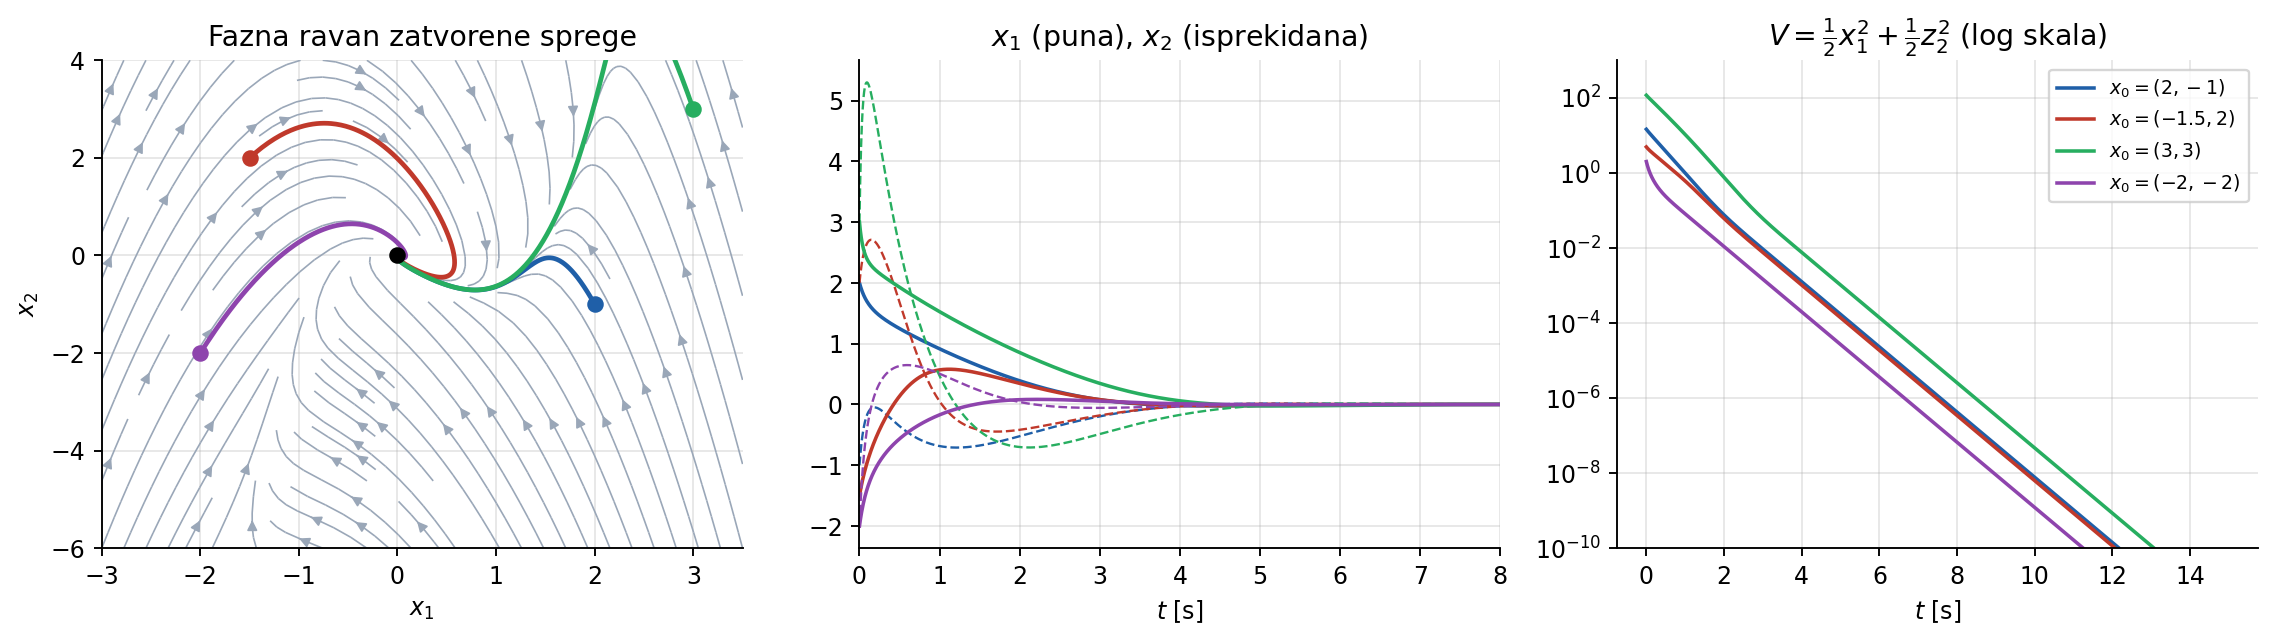
\includegraphics[width=1\linewidth,height=\textheight,keepaspectratio,alt={Domaći 4.2: sve trajektorije završe u nuli (levo i u sredini); desno se vidi da V opada kao prava linija na logaritamskoj skali, tj. eksponencijalno, kako teorija predviđa. Iz udaljenih početnih stanja upravljanje je veliko (do 87 iz (3, 3)), što je cena poništavanja nelinearnosti}]{figures/nel_backstepping.png}
\caption{Domaći 4.2: sve trajektorije završe u nuli (levo i u sredini); desno se vidi da V opada kao prava linija na logaritamskoj skali, tj. eksponencijalno, kako teorija predviđa. Iz udaljenih početnih stanja upravljanje je veliko (do 87 iz (3, 3)), što je cena poništavanja nelinearnosti}
\end{figure}

U Matlabu: \texttt{ode45} sa desnom stranom \texttt{{[}x1\^{}2\ -\ x1\^{}3\ +\ x2;\ u(\allowbreak{}x1,\allowbreak{}\ x2){]}}, crtati \(x_1(t)\), \(x_2(t)\), \(u(t)\) i \(V(t)\). Da \(V\) monotono opada je najbolja provera da je izvođenje tačno.

\subsubsection{Pitanja na odbrani (4.2)}

\begin{enumerate}
\def\labelenumi{\arabic{enumi}.}
\item \textbf{Zašto backstepping, a ne linearizacija u povratnoj sprezi?} I linearizacija bi ovde radila (\(y = x_1\), \(\rho = 2 = n\)), ali poništava \textbf{sve} nelinearnosti, i korisno \(-x_1^3\). Backstepping ga zadržava i usput daje Ljapunovljevu funkciju koja dokazuje globalnu stabilnost.
\item \textbf{Zašto \(\phi = -x_1^2 - x_1\), a ne \(-x_1^2 + x_1^3 - x_1\)?} Član \(-x_1^3\) već stabilizuje (troši „energiju'' za veliko \(|x_1|\)); poništavanje bi tražilo upravljanje reda \(x_1^3\) bez ikakve koristi.
\item \textbf{Da li je \(-x_1\) u \(\phi\) neophodan?} Nije za stabilnost: \(\dot x_1 = -x_1^3\) je asimptotski stabilno (\(\dot V_1 = -x_1^4\)), ali sporo oko nule i ne eksponencijalno. \(-x_1\) daje eksponencijalnu konvergenciju.
\item \textbf{Objasnite svaki član upravljanja.} \(-(1 + 2x_1)(x_1^2 - x_1^3 + x_2)\) poništava \(-\dot\phi\) u \(\dot z_2\); \(-x_1\) poništava unakrsni član \(x_1z_2\) iz \(\dot V_1\); \(-kz_2\) daje prigušenje greške.
\item \textbf{Šta ako promenite \(k\)?} Za svako \(k > 0\) ostaje GAS. Veće \(k\) brže gasi \(z_2\), ali \(x_1\) ne ubrzava mnogo, jer njegovu brzinu određuje \(\phi\) (\(\dot x_1 = -x_1 - x_1^3 + z_2\)). Vidi sliku u 4.1.
\item \textbf{Zašto je stabilnost globalna, a ne samo lokalna?} \(V\) je radijalno neograničena, \(\dot V\) negativno definitna na celom \(\mathbb{R}^2\), a veza \((x_1, x_2) \leftrightarrow (x_1, z_2)\) je globalno invertibilna.
\item \textbf{Kako Matlab potvrđuje izvođenje?} \(V(t)\) monotono opada za sva početna stanja; na log skali pada bar kao \(e^{-2t}\). Greška u znaku u izvođenju bi se odmah videla kao rast \(V\).
\item \textbf{Zašto je upravljanje iz \((3, 3)\) čak 87?} Daleko od nule poništavanje člana \((1 + 2x_1)(x_1^2 - x_1^3 + x_2)\) je skupo: \(u(0) = 7 \cdot 15 - 3 - 15 = 87\). U praksi bi aktuator ušao u zasićenje, pa globalna garancija više ne bi važila.
\item \textbf{Šta je strict-feedback oblik i zašto ga ovaj sistem ima?} Svaka jednačina zavisi samo od stanja do nje i od sledećeg stanja (linearno). Ovde \(\dot x_1\) zavisi od \(x_1\) i \(x_2\), a \(\dot x_2 = u\).
\end{enumerate}

\subsection{Domaći 4.1: simulacija primera iz Khalil-a}

Predavanja nisu snimljena, a profesor na njima radi primere iz knjige. Zato se simuliraju \textbf{primeri integratorskog backstepping-a iz Khalil-a, odeljak 14.3}: primer 14.8 (sistem drugog reda) i primer 14.9 (isti sistem sa dodatim integratorom) {[}Khalil 3. izd.; odelj. 14.3; proveriti broj primera u knjizi{]}. Primer 14.8 je isti sistem kao zadatak 4.2; u 4.1 se simulira tačno Khalilov zakon (\(k = 1\)) i ispituje uticaj \(k\), a primer 14.9 pokazuje rekurzivni korak.

\subsubsection{Primer A (Khalil 14.8): sistem drugog reda}

\[\dot x_1 = x_1^2 - x_1^3 + x_2, \qquad \dot x_2 = u\]

Izvođenje je korak po korak dato u 4.2. Ukratko:

\begin{enumerate}
\def\labelenumi{\arabic{enumi}.}
\item \(x_2\) je virtuelno upravljanje: \(\phi_1(x_1) = -x_1^2 - x_1\), \(V_1 = \frac12x_1^2\), \(\dot V_1 = -x_1^2 - x_1^4\).
\item Greška \(z_2 = x_2 - \phi_1 = x_2 + x_1 + x_1^2\), pa je \(\dot x_1 = -x_1 - x_1^3 + z_2\) i \(\dot z_2 = u + (1 + 2x_1)(x_1^2 - x_1^3 + x_2)\).
\item \(V = V_1 + \frac12z_2^2\) daje \(\dot V = -x_1^2 - x_1^4 + z_2\left[x_1 + u + (1 + 2x_1)(x_1^2 - x_1^3 + x_2)\right]\).
\item Zagrada se izjednači sa \(-kz_2\); Khalil uzima \(k = 1\):
\end{enumerate}

\[u = \phi_2(x_1, x_2) = -(1 + 2x_1)(x_1^2 - x_1^3 + x_2) - x_1 - (x_2 + x_1 + x_1^2)\]

\[V(x) = \frac12x_1^2 + \frac12(x_2 + x_1 + x_1^2)^2, \qquad \dot V = -x_1^2 - x_1^4 - (x_2 + x_1 + x_1^2)^2\]

\textbf{Šta simulirati:} zatvorenu spregu za \(k = 1\) iz početnih stanja kao u 4.2, pa isto za veće \(k\) (npr. \(k = 5\)). Crtati \(x_1(t)\), grešku \(z_2(t)\) i \(u(t)\).

\textbf{Šta slike treba da pokažu:} sva stanja idu u nulu; sa većim \(k\) greška \(z_2\) nestaje mnogo brže (skoro kao \(e^{-kt}\)), ali \(x_1\) ubrza samo malo, jer brzinu \(x_1\) diktira virtuelni zakon \(\phi_1\), a ne \(k\). Veće \(k\) ne znači uvek veće upravljanje: iz \((2, -1)\) je \(u(0) = 23 - 5k\) (moduo opada sa \(k\)), a iz \((0{,}5;\ 0{,}5)\) je \(u(0) = -1{,}75 - 1{,}25k\) (moduo raste sa \(k\)).

\begin{figure}
\centering
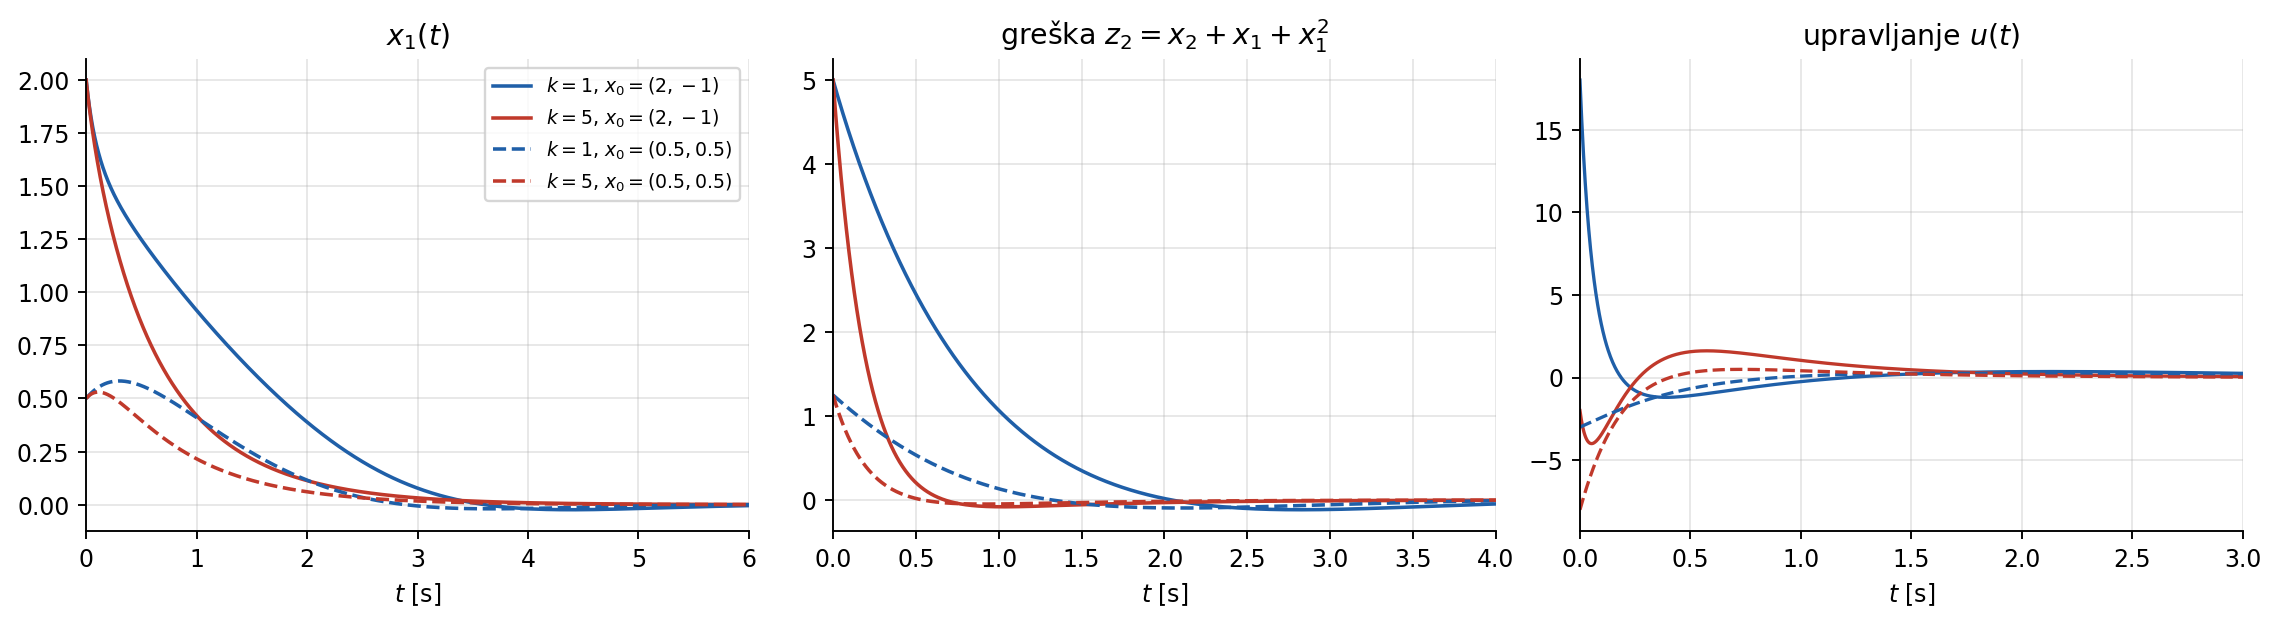
\includegraphics[width=1\linewidth,height=\textheight,keepaspectratio,alt={Khalil primer 14.8 sa k = 1 (plavo) i k = 5 (crveno), iz (2, −1) (puno) i (0,5; 0,5) (isprekidano): greška z₂ (sredina) sa većim k nestaje mnogo brže, a x₁ (levo) se ubrza tek malo; upravljanje (desno) iz (2, −1) je sa k = 5 manje (18 → 4), a iz (0,5; 0,5) veće (3 → 8)}]{figures/nel_bs_148_k.png}
\caption{Khalil primer 14.8 sa k = 1 (plavo) i k = 5 (crveno), iz (2, −1) (puno) i (0,5; 0,5) (isprekidano): greška z₂ (sredina) sa većim k nestaje mnogo brže, a x₁ (levo) se ubrza tek malo; upravljanje (desno) iz (2, −1) je sa k = 5 manje (18 → 4), a iz (0,5; 0,5) veće (3 → 8)}
\end{figure}

\subsubsection{Primer B (Khalil 14.9): dodat integrator}

\[\dot x_1 = x_1^2 - x_1^3 + x_2, \qquad \dot x_2 = x_3, \qquad \dot x_3 = u\]

Sada \(u\) deluje na \(x_3\), a \(x_3\) na podsistem iz primera A. Ideja: ceo podsistem \((x_1, x_2)\) je „\(\eta\)„, a \(x_3\) je „\(\xi\)„ iz integratorskog backstepping-a. Za taj podsistem već imamo sve iz primera A.

\textbf{Korak 1: virtuelno upravljanje za \(x_3\).} Uz \(\eta = [x_1, x_2]^T\) i \(\xi = x_3\):

\[\dot\eta = \underbrace{\begin{bmatrix} x_1^2 - x_1^3 + x_2 \\ 0 \end{bmatrix}}_{f(\eta)} + \underbrace{\begin{bmatrix} 0 \\ 1 \end{bmatrix}}_{g}x_3\]

To je sistem iz primera A sa \(x_3\) umesto \(u\). Zato je stabilizujući virtuelni zakon upravo \(\phi_2(x_1, x_2)\) iz primera A, a njegova Ljapunovljeva funkcija je \(V(x_1, x_2)\) odatle, sa \(\dot V = -x_1^2 - x_1^4 - z_2^2\) kada je \(x_3 = \phi_2\).

\textbf{Korak 2: nova greška.}

\[z_3 = x_3 - \phi_2(x_1, x_2)\]

Pošto je \(x_3 = \phi_2 + z_3\), jednačina za \(x_2\) postaje \(\dot x_2 = \phi_2 + z_3\). Izvod greške:

\[\dot z_3 = u - \dot\phi_2 = u - \frac{\partial\phi_2}{\partial x_1}(x_1^2 - x_1^3 + x_2) - \frac{\partial\phi_2}{\partial x_2}x_3\]

Parcijalni izvodi od \(\phi_2 = -(1 + 2x_1)(x_1^2 - x_1^3 + x_2) - x_1 - (x_2 + x_1 + x_1^2)\) (za prvi član pravilo proizvoda):

\[
\begin{aligned}
\frac{\partial\phi_2}{\partial x_1} &= -2(x_1^2 - x_1^3 + x_2) - (1 + 2x_1)(2x_1 - 3x_1^2) - 1 - (1 + 2x_1) \\
&= -2(x_1^2 - x_1^3 + x_2) - (1 + 2x_1)(2x_1 - 3x_1^2) - 2 - 2x_1 \\
\frac{\partial\phi_2}{\partial x_2} &= -(1 + 2x_1) - 1 = -2(1 + x_1)
\end{aligned}
\]

\textbf{Korak 3: kompozitna funkcija.}

\[V_c = V(x_1, x_2) + \frac12z_3^2\]

Kada je \(x_3 = \phi_2 + z_3\), izvod \(V\) dobija dodatni član samo zbog \(z_3\) u \(\dot x_2\): \(\frac{\partial V}{\partial x_2}z_3\), gde je \(\frac{\partial V}{\partial x_2} = x_2 + x_1 + x_1^2 = z_2\). Zato

\[\dot V_c = -x_1^2 - x_1^4 - z_2^2 + z_3\left[z_2 + u - \dot\phi_2\right]\]

\textbf{Korak 4: upravljanje.} Zagrada se izjednači sa \(-kz_3\):

\begin{kljucna}
\[u = \frac{\partial\phi_2}{\partial x_1}(x_1^2 - x_1^3 + x_2) - 2(1 + x_1)x_3 - (x_2 + x_1 + x_1^2) - k\left[x_3 - \phi_2(x_1, x_2)\right]\]
\[\dot V_c = -x_1^2 - x_1^4 - z_2^2 - kz_3^2 < 0 \quad \text{za } x \ne 0\]
\end{kljucna}

Khalil ponovo uzima \(k = 1\). Članovi imaju istu ulogu kao ranije: prva dva poništavaju \(\dot\phi_2\), treći poništava unakrsni član \(z_2z_3\), a četvrti prigušuje \(z_3\). Preslikavanje \((x_1, x_2, x_3) \to (x_1, z_2, z_3)\) je trougaono i globalno invertibilno, a \(V_c = \frac12(x_1^2 + z_2^2 + z_3^2)\) je radijalno neograničena, pa je nula \textbf{globalno asimptotski stabilna}. Za \(k \ge 1\) je \(\dot V_c \le -(x_1^2 + z_2^2 + z_3^2) = -2V_c\), pa \(V_c\) opada bar kao \(e^{-2t}\).

U Matlabu (skica, \texttt{ode45}, uz zadato \texttt{k}):

\begin{verbatim}
f1  = @(x) x(1)^2 - x(1)^3 + x(2);
ph2 = @(x) -(1+2*x(1))*f1(x) - x(1) - (x(2)+x(1)+x(1)^2);
d1  = @(x) -2*f1(x) - (1+2*x(1))*(2*x(1)-3*x(1)^2) - 2 - 2*x(1);
u   = @(x) d1(x)*f1(x) - 2*(1+x(1))*x(3) - (x(2)+x(1)+x(1)^2) - k*(x(3)-ph2(x));
rhs = @(t,x) [f1(x); x(3); u(x)];
[t, X] = ode45(rhs, [0 20], [1; 0; 0]);
\end{verbatim}

\textbf{Šta simulirati:} nekoliko početnih stanja, npr. \((1, 0, 0)\), \((-1, 1, 0)\) i \((0{,}5;\ -1;\ 2)\), sa \(k = 1\). Crtati \(x_1, x_2, x_3\) u vremenu, \(u(t)\) i \(V_c(t)\) na log skali.

\textbf{Šta slike treba da pokažu:} sva tri stanja idu u nulu za oko 5 s; \(V_c\) monotono opada, na log skali skoro kao prava (nagib oko \(e^{-2t}\)); upravljanje je na početku veće nego kod sistema drugog reda (do 31 iz \((-1, 1, 0)\)), jer \(x_3\) mora brzo da stigne do \(\phi_2\), koje je daleko od nule veliko. Provereno simulacijom u Python-u (\texttt{make\_\allowbreak{}figures\_\allowbreak{}bs.py}): posle 20 s je \(\|x\| < 10^{-8}\) za sva tri početna stanja, a \(V_c\) monotono opada.

\begin{figure}
\centering
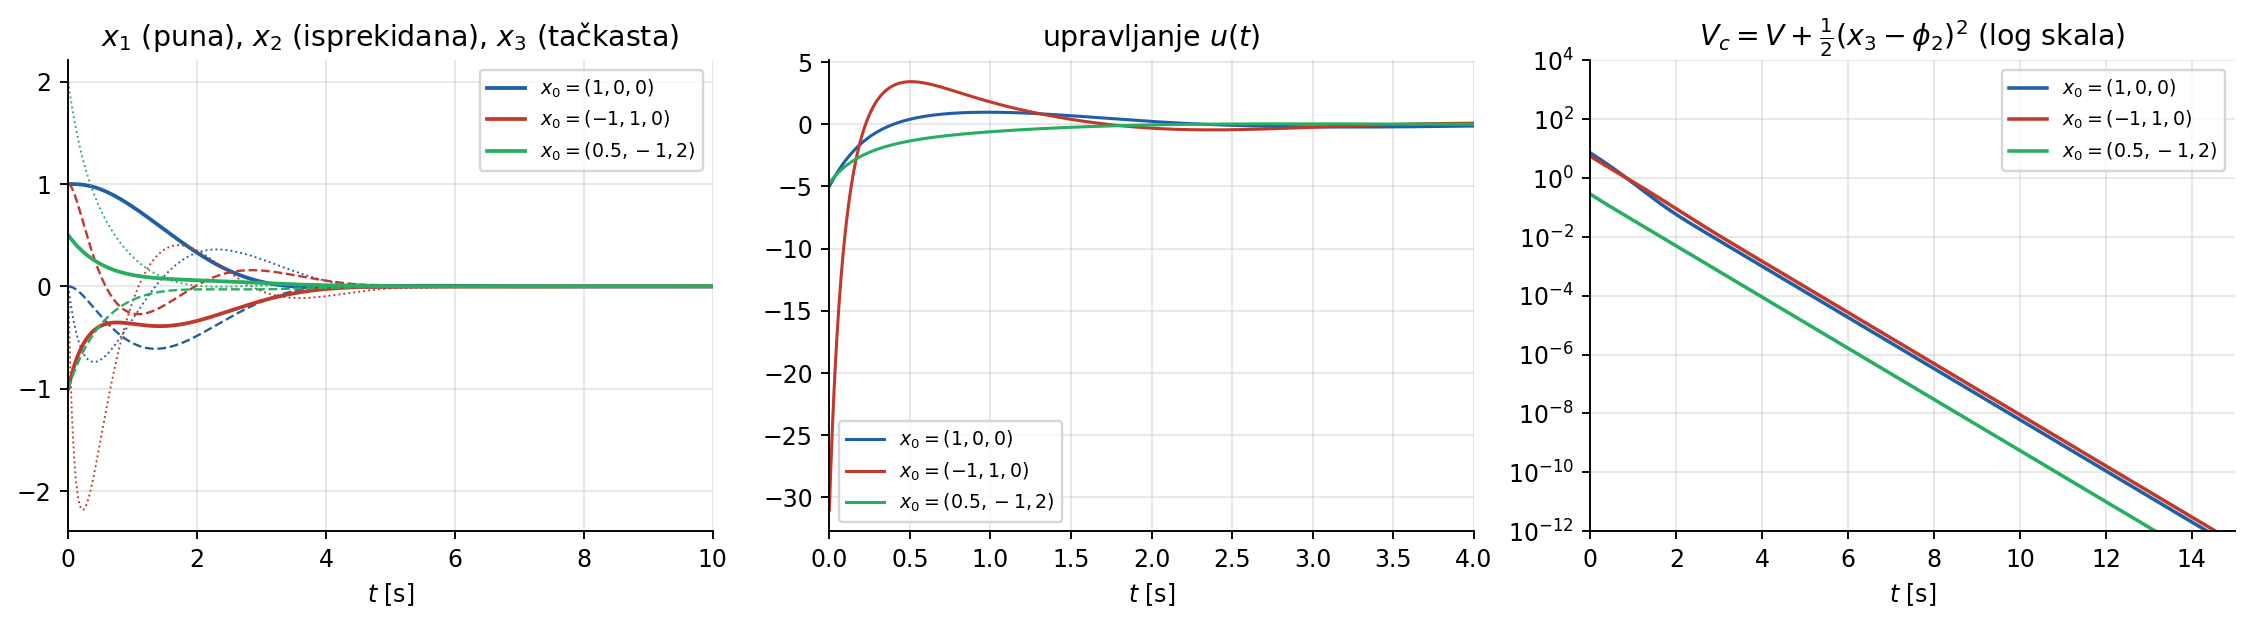
\includegraphics[width=1\linewidth,height=\textheight,keepaspectratio,alt={Khalil primer 14.9 (k = 1), tri početna stanja: sva stanja (levo) idu u nulu, a x₃ (tačkasto) ima najveći prelazni proces jer prati virtuelni zakon φ₂; upravljanje (sredina) je najveće na početku; Vc (desno) monotono opada, na log skali skoro kao prava, tj. eksponencijalno}]{figures/nel_bs_149.png}
\caption{Khalil primer 14.9 (k = 1), tri početna stanja: sva stanja (levo) idu u nulu, a x₃ (tačkasto) ima najveći prelazni proces jer prati virtuelni zakon φ₂; upravljanje (sredina) je najveće na početku; Vc (desno) monotono opada, na log skali skoro kao prava, tj. eksponencijalno}
\end{figure}

\subsubsection{Pitanja na odbrani (4.1)}

\begin{enumerate}
\def\labelenumi{\arabic{enumi}.}
\item \textbf{Koje primere ste simulirali i zašto baš njih?} Primere integratorskog backstepping-a iz Khalil-a, odeljak 14.3 (14.8 i 14.9), jer predavanja prate knjigu, a primeri sa table nisu sačuvani.
\item \textbf{Kako se primer 14.9 nadovezuje na 14.8?} Dodat je integrator: ceo zakon iz 14.8 postaje virtuelno upravljanje \(\phi_2\) za \(x_3\), a njegova \(V\) postaje \(V\) za sledeći korak. To je jedan rekurzivni korak backstepping-a.
\item \textbf{Zašto je upravljanje u 14.9 mnogo složenije?} Mora da poništi \(\dot\phi_2\), a \(\phi_2\) već sadrži izvod od \(\phi_1\); sa svakim integratorom izrazi rastu (izvodi izvoda).
\item \textbf{Da li mora \(k = 1\)?} Ne; svako \(k > 0\) daje \(\dot V_c < 0\). Khalil uzima 1 radi jednostavnosti. Veće \(k\) brže gasi poslednju grešku, ali ne ubrzava mnogo ostala stanja.
\item \textbf{Šta tačno pokazuje slika \(V_c\) na log skali?} Da \(V_c\) monotono opada (potvrda da je izvođenje tačno), i to eksponencijalno: za \(k \ge 1\) je \(\dot V_c \le -2V_c\).
\item \textbf{Zašto \(x_3\) ima najveći prelazni proces?} Upravljanje prvo tera \(x_3\) ka \(\phi_2(x_1, x_2)\), a \(\phi_2\) je na početku veliko; tek kad je \(z_3\) malo, \(x_2\) i \(x_1\) se smiruju po zakonu iz 14.8.
\item \textbf{Da li je stabilnost u 14.9 globalna?} Da: \(V_c = \frac12(x_1^2 + z_2^2 + z_3^2)\) je radijalno neograničena, \(\dot V_c\) negativno definitna, a promena koordinata je globalna.
\item \textbf{Šta bi bilo sa još jednim integratorom?} Isti postupak još jednom: zakon iz 14.9 postaje virtuelno upravljanje za \(x_4\), a \(V_c\) se proširi sa \(\frac12z_4^2\).
\end{enumerate}

\begin{ispit}
Umeti izvesti 4.2 korak po korak i objasniti svaki član upravljanja: poništavanje \(\dot\phi\), poništavanje unakrsnog člana \(x_1z_2\), prigušenje \(-kz_2\). Obavezno reći zašto je \(-x_1^3\) zadržan i zašto je stabilnost \textbf{globalna} (\(V\) radijalno neograničena, \(\dot V\) negativno definitno). Znati šta je strict-feedback oblik i čime se backstepping razlikuje od linearizacije u povratnoj sprezi. Za 4.1 umeti objasniti kako se primer 14.9 dobija iz 14.8 (zakon iz 14.8 postaje virtuelno upravljanje) i šta pokazuju slike.
\end{ispit}

\end{document}
